% !TeX spellcheck = en_US
%
% LaTeX source file of DynELA FEM code Documentation
%
% (c) by Olivier Pantalé 2020
%
\documentclass[11pt,french,english,twoside]{book}
%
% macrosHyperlink TeX configuration file
%
% (c) by Olivier Pantalé 2020
%
%@!CODEFILE = macrosHyperlinkEnglish.tex

\usepackage{kurier} % Set the default font for the document
\usepackage{helvet}
\usepackage[T1]{fontenc}
\usepackage[utf8]{inputenc}
\usepackage[a4paper]{geometry}
\pagestyle{headings}
\setcounter{secnumdepth}{4}
\setcounter{tocdepth}{4}
\setlength{\parskip}{\medskipamount}
\setlength{\parindent}{0pt}
\usepackage{color}
\usepackage{array}
\usepackage{babel}
\usepackage{longtable}
\usepackage{multirow}
\usepackage{float}
\usepackage{textcomp}
\usepackage{amsmath}
\usepackage{amssymb}
\usepackage{cancel}
\usepackage{stmaryrd}
\usepackage{graphicx}
\PassOptionsToPackage{normalem}{ulem}
\usepackage{ulem}
\usepackage{float}
\usepackage{cite}
\usepackage{lettrine} 
\usepackage{pict2e}
\usepackage{minitoc}
\usepackage{comment}
\usepackage{tikz}
\usepackage{titletoc}
\usepackage{calc}
\usepackage{makeidx}
\usepackage{index}
\usepackage[]{titlesec} 
\usepackage{placeins}
\usepackage{tcolorbox}
\usepackage{tabularx}
\usepackage{array}
\usepackage{colortbl}
\usepackage{fancyhdr}
\usepackage{tablefootnote}
\usepackage[nice]{nicefrac}
\usetikzlibrary{shadows.blur}
\tcbuselibrary{skins}

% Define the macros for color tables
\newcolumntype{L}{>{\raggedleft\arraybackslash}X}
\newcolumntype{R}{>{\raggedright\arraybackslash}X}
\newcolumntype{C}{>{\centering\arraybackslash}X}
\tcbset{myTab/.style={enhanced,fonttitle=\bfseries,fontupper=\normalsize,
colback=gray!10!white,colframe=gray!85!black,colbacktitle=gray,
coltitle=white,center title}}

% Sets the caption of all figures
\usepackage{caption}
\captionsetup[figure]{labelfont={bf,it}, textfont=it}
\captionsetup[table]{labelfont={bf,it}, textfont=it}

% Change the list spaces
\usepackage{enumitem}
\setlist[description]{itemsep=0.3em, parsep=0em, itemindent=-1em}

\makeatletter

% Titre de l'ouvrage
\newcommand{\MyTitle}{DynELA FEM code v.4.0}

%Command for bilingual texts
\newcommand{\frEn}[2]{#2} % Default English

% Command for Full version
\newenvironment{fullVersion}{}{}

% Definition of pages sizes and geometry
\geometry{verbose, a4paper, tmargin=3cm, bmargin=2.5cm, lmargin=2cm, rmargin=2cm, headheight=1cm, headsep=1cm, footskip=1cm}
\pagestyle{fancyplain}
\renewcommand{\floatpagefraction}{1.0}
\renewcommand{\textfraction}{0.2}
\renewcommand{\bottomfraction}{1.0}
\setcounter{tocdepth}{2}
\setcounter{secnumdepth}{3}

% Defintiion of the Lettrine
\newcommand{\LETTRINE}[1]{\lettrine[lines=3]{\textcolor{myRed}{#1}}{}}

% Special style for footnotes
\renewcommand\@makefnmark{\@textsuperscript{\normalfont(\@thefnmark)}}

% Special style for references
\newcommand{\myCite}[1]{\textbf{\underbar{\cite{#1}~}}}

% Bibliography enhancement
\renewenvironment{thebibliography}[1]
     {\section*{\bibname}%
      \@mkboth{\MakeUppercase\bibname}{\MakeUppercase\bibname}%
      \list{\@biblabel{\@arabic\c@enumiv}}%
           {\settowidth\labelwidth{\@biblabel{#1}}%
            \leftmargin\labelwidth
            \advance\leftmargin\labelsep
            \@openbib@code
            \usecounter{enumiv}%
            \let\p@enumiv\@empty
            \renewcommand\theenumiv{\@arabic\c@enumiv}}%
      \sloppy
      \clubpenalty4000
      \@clubpenalty \clubpenalty
      \widowpenalty4000%
      \sfcode`\.\@m}
     {\def\@noitemerr
       {\@latex@warning{Empty `thebibliography' environment}}%
      \endlist}

\renewcommand{\chaptermark}[1]{\markboth{#1}{}}
\lhead [\fancyplain {\bfseries\thepage} {\bfseries\thepage \\ \textcolor{myGray}{\rule{\textwidth}{2mm}}}]
       {\fancyplain {} {\bfseries\leftmark \\ \textcolor{myGray}{\rule{\textwidth}{2mm}}}}
\rhead [\fancyplain {} {\bfseries\leftmark \\ \textcolor{myGray}{\rule{\textwidth}{2mm}}}]
       {\fancyplain {\bfseries\thepage} {\bfseries\thepage \\ \textcolor{myGray}{\rule{\textwidth}{2mm}}}}
\chead{}
\cfoot{}
\lfoot [{\textcolor{myGray}{\rule{\textwidth}{2mm}}\\ \mbox{\scriptsize{\MyTitle}}}]
       {\textcolor{myGray}{\rule{\textwidth}{2mm}}\\ \mbox{\scriptsize{Olivier PANTALE}}}
\rfoot [{\textcolor{myGray}{\rule{\textwidth}{2mm}}\\ \mbox{\scriptsize{Olivier PANTALE}}}]
       {\textcolor{myGray}{\rule{\textwidth}{2mm}}\\ \mbox{\scriptsize{\MyTitle}}}
\renewcommand{\headrulewidth}{0pt}
\renewcommand{\footrulewidth}{0pt}

% cette ligne est necessaire si il n'y a pas d'algorithme dans le fichier lyx
\@ifundefined{algorithm}{
\newfloat{algorithm}{htbp}{loa}
}

% dfinitions pour les sections en couleur dans le texte
\renewcommand\section{\@startsection {section}{1}{\z@}%
                                   {-3.5ex \@plus -1ex \@minus -.2ex}%
                                   {2.3ex \@plus.2ex}%
                                   {\normalfont\LARGE\bfseries\color{myRed}}}
\renewcommand\subsection{\@startsection{subsection}{2}{\z@}%
                                     {-3.25ex\@plus -1ex \@minus -.2ex}%
                                     {1.5ex \@plus .2ex}%
                                     {\normalfont\Large\bfseries\color{myRed}}}
\renewcommand\subsubsection{\@startsection{subsubsection}{3}{\z@}%
                                     {-3.25ex\@plus -1ex \@minus -.2ex}%
                                     {1.5ex \@plus .2ex}%
                                     {\normalfont\large\bfseries\color{myRed}}}

% le super format pour les chapitres
\colorlet{chpnumbercolor}{black}
\let\oldl@chapter\l@chapter
\def\l@chapter#1#2{\oldl@chapter{#1}{\textcolor{chpnumbercolor}{#2}}}

\let\old@dottedcontentsline\@dottedtocline
\def\@dottedtocline#1#2#3#4#5{%
\old@dottedcontentsline{#1}{#2}{#3}{#4}{{\textcolor{chpnumbercolor}{#5}}}}

\titleformat{\chapter}[display]
  {\normalfont\color{myRed}}
  {\filleft\Huge\sffamily\bfseries\chaptertitlename\hspace*{2mm}%
  \begin{tikzpicture}[baseline={([yshift=-.6ex]current bounding box.center)}]
    \node[fill=myRed, circle, text=white] {\thechapter};
  \end{tikzpicture}}
  {1ex}
  {\titlerule[5pt]\vspace*{2ex}\huge\sffamily\itshape}
  []

\titleformat{name=\chapter, numberless}[display]
  {\normalfont\color{myRed}}
  {}
  {1ex}
  {\vspace*{2ex}\huge\sffamily\itshape}
  []

% Command to print the actual minitoc
\newcommand{\printmyminitoc}[1][2]{%
    \vspace*{-5ex}
%    \noindent\hspace*{-0.5\hoffset}\hspace*{-0.5in}\hspace*{-0.5\oddsidemargin}%
    \colorlet{chpnumbercolor}{myRed}%
    \begin{tikzpicture}
    \node[rounded corners, align=left, fill=myGray80, inner sep=5mm]{%
        \color{myRed}%
        \begin{minipage}{0.95\columnwidth}%minipage trick
        \printcontents[chapters]{}{1}{\setcounter{tocdepth}{#1}}
        \end{minipage}};
    \end{tikzpicture}
    \vspace*{5ex}}

\def\@part[#1]#2{%
    \ifnum \c@secnumdepth >-2\relax
      \refstepcounter{part}%
      \addcontentsline{toc}{part}{\thepart\hspace{1em}#1}%
    \else
      \addcontentsline{toc}{part}{#1}%
    \fi
    \markboth{}{}%
    {\centering
     \interlinepenalty \@M
    \textcolor{myRed}{\rule{0.5\textwidth}{4mm}}%  <--- the rule
    \nobreak
    \vskip 5\p@
    \normalfont
     \ifnum \c@secnumdepth >-2\relax
       \huge\bfseries \color{myRed}\partname~\thepart
       \par
       \vskip 20\p@
     \fi
     \Huge \bfseries #2\par}%
    \vskip 5\p@
    \textcolor{myRed}{\rule{\textwidth}{4mm}}%  <--- the rule
    \nobreak
    \vskip 10\p@
    \@endpart}

\def\@endpart{\vfil\newpage
	\setcounter{chapter}{0} %reset the counter between chapters
              \if@twoside
               \if@openright
                \null
                \thispagestyle{empty}%
                \newpage
               \fi
              \fi
              \if@tempswa
                \twocolumn
              \fi}

% creation des programmes
\floatstyle{ruled}
\newfloat{Program}{thp}{lop}[chapter]

% plus de place dans les listes
\renewcommand*\l@figure{\@dottedtocline{1}{1.5em}{3.3em}}
\renewcommand*\l@table{\@dottedtocline{1}{1.5em}{3.3em}}
\renewcommand\listof[2]{%
  \@ifundefined{ext@#1}{\float@error{#1}}{%
    \@ifundefined{chapter}{\def\@tempa{\section*}}%
      {\def\@tempa{\chapter*}}%
    \@tempa{#2\@mkboth{\uppercase{#2}}{\uppercase{#2}}}%
    \@namedef{l@#1}{\@dottedtocline{1}{1.5em}{3.3em}}%
    \@starttoc{\@nameuse{ext@#1}}}}

\AtBeginDocument{
\addto\captionsfrench{
\renewcommand{\figurename}{Figure }
\renewcommand{\tablename}{Tableau }
}}

% les numros incluent le numro de la partie
\renewcommand \thefigure
     {\ifnum \c@part>\z@ \thepart.\fi \ifnum \c@chapter>\z@ \thechapter.\fi \@arabic\c@figure}
\renewcommand \thetable
     {\ifnum \c@part>\z@ \thepart.\fi \ifnum \c@chapter>\z@ \thechapter.\fi \@arabic\c@table}

%Definition des mises en page
\newcommand{\listingfontsscale}{\footnotesize}

%
% macrosGene TeX configuration file
%
\usepackage{esvect}
\usepackage{keystroke}
\usepackage{xstring}
\usepackage{transparent}
\usepackage{xspace}
\usepackage{color}
\usepackage{pdfpages}

% Define the set of colors
\definecolor{myGray}{gray}{0.75}
\definecolor{myGray90}{gray}{0.90}
\definecolor{myGray80}{gray}{0.80}
\definecolor{myGray50}{gray}{0.50}
\definecolor{myGray40}{gray}{0.40}
\definecolor{myRed}{rgb}{0.34,0.05,0.05}  
\definecolor{myLightRed}{rgb}{0.54,0.05,0.05}  
\definecolor{myDarkRed}{rgb}{0.14,0.05,0.05} 
\definecolor{myBlue}{rgb}{0.05,0.05,0.34}  % Blue color
\definecolor{myGreen}{rgb}{0.05,0.34,0.05}  % Green color

% Command to define two texts depending on the current language
\newcommand{\FrEn}[2]{\IfStrEq*{\languagename}{french}{#1}{#2}}

% Redefine the esvector shape to remove overlapping
\def\traitfill@#1#2#3#4{%
  $\m@th\mkern2mu\relax#4#1\mkern-1.5mu %on met \relbaredd au d\'ebut
   \cleaders\hbox{$#4\mkern-0.3mu#2\mkern-0.3mu$}\hfill %remplit avec relbareda
   \mkern-1.5mu#3$%
}

% affect overrightarrow to vv
\renewcommand{\overrightarrow}{\vv}

% définition des commandes locales
% Definition of the C++ special command
\DeclareRobustCommand{\Cpp}
{\valign{\vfil\hbox{##}\vfil\cr 
   \textsf{C\kern-.1em}\cr
   $\hbox{\fontsize{\ssf@size}{0}\textbf{+\kern-0.05em+}}$\cr}\xspace%
}

% Definition des listings avec langage par défaut Python
\usepackage{listings}

\lstnewenvironment{CppListing}[1][]
    {\lstset{language=C++,
	keywordstyle=\color{myRed},
	numberstyle=\footnotesize\color{myGray50},
	numbers=left,
	frame=single,xleftmargin=5.0ex,xrightmargin=1.0ex,
	literate={-} { \textrm{-}}{1},
	%otherkeywords={>>>},
	%morekeywords={as,assert,with,yield},
	commentstyle=\color{myGray40},
	stringstyle=\color{myGreen},
	basicstyle=\listingfontsscale\sffamily\upshape,
	escapeinside={(*}{*)},  
	backgroundcolor=\color{myGray90},
	rulecolor=\color{myGray50},
        #1}%
        \noindent\begin{minipage}{\textwidth}\csname\@lst @SetFirstNumber\endcsname\end{minipage}}
        {\csname\@lst @SaveFirstNumber\endcsname}

\lstnewenvironment{FortranListing}[1][]
    {\lstset{language=[77]Fortran,
	keywordstyle=\color{myRed},
	numberstyle=\footnotesize\color{myGray50},
	numbers=left,
	frame=single,xleftmargin=5.0ex,xrightmargin=1.0ex,
	literate={-} { \textrm{-}}{1},
	%otherkeywords={>>>},
	%morekeywords={as,assert,with,yield},
	commentstyle=\color{myGray50},
	stringstyle=\color{myGreen},
	basicstyle=\listingfontsscale\sffamily\upshape,
	escapeinside={(*}{*)},  
	backgroundcolor=\color{myGray90},
	rulecolor=\color{myGray50},
        #1}%
        \noindent\begin{minipage}{\textwidth}\csname\@lst @SetFirstNumber\endcsname\end{minipage}}
        {\csname\@lst @SaveFirstNumber\endcsname}

\lstnewenvironment{PythonListing}[1][]
    {\lstset{language=Python,
	keywordstyle=\color{myRed},
	numberstyle=\footnotesize\color{myGray50},
	numbers=left,
	frame=single,xleftmargin=5.0ex,xrightmargin=1.0ex,
	%float=h,
	literate={-} { \textrm{-}}{1},
	%otherkeywords={>>>},
	morekeywords={as,assert,with,yield},
	commentstyle=\color{myGray40},
	stringstyle=\color{myGreen},
	basicstyle=\listingfontsscale\sffamily\upshape,
	escapeinside={(*}{*)},  
	backgroundcolor=\color{myGray90},
	rulecolor=\color{myGray50},
        #1}%
        \noindent\begin{minipage}{\textwidth}\csname\@lst @SetFirstNumber\endcsname\end{minipage}}
        {\csname\@lst @SaveFirstNumber\endcsname}

\lstnewenvironment{AbaqusListing}[1][]
    {\lstset{language=Python,
	keywordstyle=\color{myRed},
	numberstyle=\footnotesize\color{myGray50},
	numbers=left,
	frame=single,xleftmargin=5.0ex,xrightmargin=1.0ex,
	literate={-} { \textrm{-}}{1},
	%otherkeywords={>>>},
	morekeywords={as,assert,with,yield},
	commentstyle=\color{myGray40},
	stringstyle=\color{myGreen},
	basicstyle=\listingfontsscale\sffamily\upshape,
	escapeinside={(*}{*)},  
	backgroundcolor=\color{myGray90},
	rulecolor=\color{myGray50},
		#1}%
        \noindent\begin{minipage}{\textwidth}\csname\@lst @SetFirstNumber\endcsname\end{minipage}}
        {\csname\@lst @SaveFirstNumber\endcsname}

\lstnewenvironment{BashListing}[1][]
	{\lstset{language=bash,
		keywordstyle=\color{myRed},
		numberstyle=\footnotesize\color{myGray50},
		numbers=left,
		frame=single,xleftmargin=5.0ex,xrightmargin=1.0ex,
		literate={-} { \textrm{-}}{1},
		%otherkeywords={>>>},
		%morekeywords={as,assert,with,yield},
		commentstyle=\color{myGray40},
		stringstyle=\color{myGreen},
		basicstyle=\sffamily\listingfontsscale\upshape,
		escapeinside={(*}{*)},  
		backgroundcolor=\color{myGray90},
		rulecolor=\color{myGray50},
		#1}%
	\noindent\begin{minipage}{\textwidth}\csname\@lst @SetFirstNumber\endcsname\end{minipage}}
{\csname\@lst @SaveFirstNumber\endcsname}

\lstset{language=Python,
keywordstyle=\color{myRed},
numberstyle=\footnotesize\color{myGray40},
numbers=left,
frame=single,xleftmargin=5.0ex,xrightmargin=1.0ex,
literate={-} { \textrm{-}}{1},
%otherkeywords={>>>},
morekeywords={as,assert,with,yield},
commentstyle=\color{myGray50},
stringstyle=\color{myGreen},
basicstyle=\listingfontsscale\sffamily\upshape,
escapeinside={(*}{*)},  
backgroundcolor=\color{white},
rulecolor=\color{myGray50}}
\newcommand{\pyout}[1]{\color{blue}\textsl{#1}}

\newcommand{\TI}[1]{\mbox{\large\ensuremath{\mathsf{#1}}}}
\newcommand{\TII}[1]{\mbox{\large\ensuremath{\mathbb{#1}}}}
\newcommand{\TiI}[1]{\mbox{\large\ensuremath{\mathcal{#1}}}}

%Domaines d'intégration
\newcommand{\Ve}	{\Omega_{x}^{e}}
\newcommand{\Se}	{\Gamma_{x}^{e}}

%Tenseur des contraintes, déformations, etc...
\newcommand{\Sig}	{\mbox{\large\ensuremath{\boldsymbol{\sigma}}}}
\newcommand{\Eps}	{\mbox{\large\ensuremath{\boldsymbol{\varepsilon}}}}
\newcommand{\Alp}	{\mbox{\large\ensuremath{\boldsymbol{\alpha}}}}
\newcommand{\ro}	{\mbox{\large\ensuremath{\boldsymbol{\rho}}}}
\newcommand{\gam}	{\mbox{\large\ensuremath{\boldsymbol{\gamma}}}}
\newcommand{\Gam}	{\mbox{\large\ensuremath{\boldsymbol{\Gamma}}}}
\newcommand{\om}	{\mbox{\large\ensuremath{\boldsymbol{\omega}}}}
\newcommand{\Om}	{\mbox{\large\ensuremath{\boldsymbol{\Omega}}}}
\newcommand{\Fi}	{\mbox{\Large\ensuremath{\boldsymbol{\phi}}}}
\newcommand{\Dev}	{\mbox{\Large\ensuremath{\mathsf{s}}}}

%Tenseur Identité
\newcommand{\IId}	{\mbox{\large\ensuremath{\mathbb{I}}}}
\newcommand{\Iid}	{\mbox{\Large\ensuremath{\mathcal{I}}}}
\newcommand{\Id}  	{\mbox{\large\ensuremath{\mathsf{1}}}}

% Tenseurs A du second, 3eme et 4eme ordre
\newcommand{\A}  	{\mbox{\large\ensuremath{\mathsf{A}}}}
\newcommand{\IiA}	{\mbox{\large\ensuremath{\mathcal{A}}}}
\newcommand{\IIA}	{\mbox{\large\ensuremath{\mathbb{A}}}}
\newcommand{\ia}	{\mbox{\large\ensuremath{\mathsf{a}}}}

%Tenseurs B du second, 3eme et 4eme ordre
\newcommand{\B}		{\mbox{\large\ensuremath{\mathsf{B}}}}
\newcommand{\IiB}	{\mbox{\large\ensuremath{\mathcal{B}}}}
\newcommand{\IIB}	{\mbox{\large\ensuremath{\mathbb{B}}}}
\newcommand{\ib}	{\mbox{\large\ensuremath{\mathsf{b}}}}

% Tenseurs C du second, 3eme et 4eme ordre
\newcommand{\C}		{\mbox{\large\ensuremath{\mathsf{C}}}}
\newcommand{\IiC}	{\mbox{\large\ensuremath{\mathcal{C}}}}
\newcommand{\IIC}	{\mbox{\large\ensuremath{\mathbb{C}}}}

% Tenseurs D du second, 3eme et 4eme ordre
\newcommand{\D}		{\mbox{\large\ensuremath{\mathsf{D}}}}
\newcommand{\IiD}	{\mbox{\large\ensuremath{\mathcal{D}}}}
\newcommand{\IID}	{\mbox{\large\ensuremath{\mathbb{D}}}}

% Tenseurs E du second, 3eme et 4eme ordre
\newcommand{\E}		{\mbox{\large\ensuremath{\mathsf{E}}}}
\newcommand{\IiE}	{\mbox{\large\ensuremath{\mathcal{E}}}}
\newcommand{\IIE}	{\mbox{\large\ensuremath{\mathbb{E}}}}
\newcommand{\e}		{\mbox{\large\ensuremath{\mathsf{e}}}}

% Tenseurs F du second, 3eme et 4eme ordre
\newcommand{\F}		{\mbox{\large\ensuremath{\mathsf{F}}}}
\newcommand{\IiF}	{\mbox{\large\ensuremath{\mathcal{F}}}}
\newcommand{\IIF}	{\mbox{\large\ensuremath{\mathbb{F}}}}
\newcommand{\f}		{\mbox{\large\ensuremath{\mathsf{f}}}}

% Tenseurs H du second, 3eme et 4eme ordre
\newcommand{\G}		{\mbox{\large\ensuremath{\mathsf{G}}}}
\newcommand{\IiG}	{\mbox{\large\ensuremath{\mathcal{G}}}}
\newcommand{\IIG}	{\mbox{\large\ensuremath{\mathbb{G}}}}
\newcommand{\ig}	{\mbox{\large\ensuremath{\mathsf{g}}}}

% Tenseurs H du second, 3eme et 4eme ordre
\newcommand{\iH}	{\mbox{\large\ensuremath{\mathsf{H}}}}
\newcommand{\IiH}	{\mbox{\large\ensuremath{\mathcal{H}}}}
\newcommand{\IIH}	{\mbox{\large\ensuremath{\mathbb{H}}}}

% Tenseurs J du second, 3eme et 4eme ordre
\newcommand{\J}		{\mbox{\large\ensuremath{\mathsf{J}}}}
\newcommand{\IiJ}	{\mbox{\large\ensuremath{\mathcal{J}}}}
\newcommand{\IIJ}	{\mbox{\large\ensuremath{\mathbb{J}}}}

% Tenseurs K du second, 3eme et 4eme ordre
\newcommand{\K}		{\mbox{\large\ensuremath{\mathsf{K}}}}
\newcommand{\IiK}	{\mbox{\large\ensuremath{\mathcal{K}}}}
\newcommand{\IIK}	{\mbox{\large\ensuremath{\mathbb{K}}}}

% Tenseurs L du second, 3eme et 4eme ordre
\newcommand{\iL}	{\mbox{\large\ensuremath{\mathsf{L}}}}
\newcommand{\IiL}	{\mbox{\large\ensuremath{\mathcal{L}}}}
\newcommand{\IIL}	{\mbox{\large\ensuremath{\mathbb{L}}}}

% Tenseurs M du second, 3eme et 4eme ordre
\newcommand{\M}		{\mbox{\large\ensuremath{\mathsf{M}}}}
\newcommand{\IiM}	{\mbox{\large\ensuremath{\mathcal{M}}}}
\newcommand{\IIM}	{\mbox{\large\ensuremath{\mathbb{M}}}}
\newcommand{\m}		{\mbox{\large\ensuremath{\mathsf{m}}}}

% Tenseurs N du second, 3eme et 4eme ordre
\newcommand{\N}		{\mbox{\large\ensuremath{\mathsf{N}}}}
\newcommand{\IiN}	{\mbox{\large\ensuremath{\mathcal{N}}}}
\newcommand{\IIN}	{\mbox{\large\ensuremath{\mathbb{N}}}}
\newcommand{\n}		{\mbox{\large\ensuremath{\mathsf{n}}}}

% Tenseurs P du second, 3eme et 4eme ordre
\newcommand{\iP}	{\mbox{\large\ensuremath{\mathsf{P}}}}
\newcommand{\IiP}	{\mbox{\large\ensuremath{\mathcal{P}}}}
\newcommand{\IIP}	{\mbox{\large\ensuremath{\mathbb{P}}}}
\newcommand{\p}		{\mbox{\large\ensuremath{\mathsf{p}}}}

% Tenseurs Q du second, 3eme et 4eme ordre
\newcommand{\Q}		{\mbox{\large\ensuremath{\mathsf{Q}}}}
\newcommand{\IiQ}	{\mbox{\large\ensuremath{\mathcal{Q}}}}
\newcommand{\IIQ}	{\mbox{\large\ensuremath{\mathbb{Q}}}}
\newcommand{\q}		{\mbox{\large\ensuremath{\mathsf{q}}}}

% Tenseurs R du second, 3eme et 4eme ordre
\newcommand{\R}		{\mbox{\large\ensuremath{\mathsf{R}}}}
\newcommand{\IiR}	{\mbox{\large\ensuremath{\mathcal{R}}}}
\newcommand{\IIR}	{\mbox{\large\ensuremath{\mathbb{R}}}}
\newcommand{\ir}	{\mbox{\large\ensuremath{\mathsf{r}}}}

% Tenseurs S du second, 3eme et 4eme ordre
\newcommand{\iS}	{\mbox{\large\ensuremath{\mathsf{S}}}}
\newcommand{\IIS}	{\mbox{\large\ensuremath{\mathbb{S}}}}
\newcommand{\IiS}	{\mbox{\Large\ensuremath{\mathcal{S}}}}

% Tenseurs T du second, 3eme et 4eme ordre
\newcommand{\T}		{\mbox{\large\ensuremath{\mathsf{T}}}}
\newcommand{\IiT}	{\mbox{\large\ensuremath{\mathcal{T}}}}
\newcommand{\IIT}	{\mbox{\large\ensuremath{\mathbb{T}}}}
\newcommand{\bt}	{\mbox{\large\ensuremath{\mathsf{t}}}}

% Tenseurs U du second, 3eme et 4eme ordre
\newcommand{\U}		{\mbox{\large\ensuremath{\mathsf{U}}}}
\newcommand{\IiU}	{\mbox{\large\ensuremath{\mathcal{U}}}}
\newcommand{\IIU}	{\mbox{\large\ensuremath{\mathbb{U}}}}
\newcommand{\iu}	{\mbox{\large\ensuremath{\mathsf{u}}}}

% Tenseurs V du second, 3eme et 4eme ordre
\newcommand{\V}		{\mbox{\large\ensuremath{\mathsf{V}}}}
\newcommand{\IiV}	{\mbox{\large\ensuremath{\mathcal{V}}}}
\newcommand{\IIV}	{\mbox{\large\ensuremath{\mathbb{V}}}}
\newcommand{\iv}	{\mbox{\large\ensuremath{\mathsf{v}}}}

% Tenseurs W du second, 3eme et 4eme ordre
\newcommand{\W}		{\mbox{\large\ensuremath{\mathsf{W}}}}
\newcommand{\IiW}	{\mbox{\large\ensuremath{\mathcal{W}}}}
\newcommand{\IIW}	{\mbox{\large\ensuremath{\mathbb{W}}}}
\newcommand{\iw}	{\mbox{\large\ensuremath{\mathsf{w}}}}

% Tenseurs X du second, 3eme et 4eme ordre
\newcommand{\X}		{\mbox{\large\ensuremath{\mathsf{X}}}}
\newcommand{\IiX}	{\mbox{\large\ensuremath{\mathcal{X}}}}
\newcommand{\x}		{\mbox{\large\ensuremath{\mathsf{x}}}}
\newcommand{\IIX}	{\mbox{\large\ensuremath{\mathbb{X}}}}

% Tenseurs Y du second, 3eme et 4eme ordre
\newcommand{\Y}		{\mbox{\large\ensuremath{\mathsf{Y}}}}
\newcommand{\IiY}	{\mbox{\large\ensuremath{\mathcal{Y}}}}
\newcommand{\y}		{\mbox{\large\ensuremath{\mathsf{y}}}}
\newcommand{\IIY}	{\mbox{\large\ensuremath{\mathbb{Y}}}}

% Tenseurs Z du second, 3eme et 4eme ordre
\newcommand{\Z}		{\mbox{\large\ensuremath{\mathsf{Z}}}}
\newcommand{\IiZ}	{\mbox{\large\ensuremath{\mathcal{Z}}}}
\newcommand{\z}		{\mbox{\large\ensuremath{\mathsf{z}}}}
\newcommand{\IIZ}	{\mbox{\large\ensuremath{\mathbb{Z}}}}

%Null tensor
\newcommand{\0}		{\mbox{\large\ensuremath{\mathsf{0}}}}

%Commandes spéciales espacements
\newcommand{\Vs}	{\vspace{1cm}}
\newcommand{\vs}	{\vspace{2mm}}

%Commandes spéciales
\newcommand{\tr}	{\mbox{\ensuremath{\mathsf{\,tr\,}}}}
\newcommand{\dev}	{\mbox{\ensuremath{\mathsf{\,dev\,}}}}
\newcommand{\grad}	{\mbox{\ensuremath{\mathsf{\,grad\,}}}}
\newcommand{\Div}	{\mbox{\ensuremath{\mathsf{\,div\,}}}}
\newcommand{\curl}	{\mbox{\ensuremath{\mathsf{\,curl\,}}}}
\renewcommand{\det}	{\mbox{\ensuremath{\mathsf{\,det\,}}}}

\newcommand{\pluseq}{\mathrel{+}=}
\newcommand{\minuseq}{\mathrel{-}=}
\newcommand{\multeq}{\mathrel{*}=}
\newcommand{\diveq}{\mathrel{/}=}

\DeclareMathAlphabet{\mathbxsl}{\encodingdefault}{\rmdefault}{m}{it}
\newcommand{\invI}[1]	{\mbox{\large\ensuremath{\mathbxsl{I_{\mathsf{#1}}}}}}
\newcommand{\invII}[1]	{\mbox{\large\ensuremath{\mathbxsl{II_{\mathsf{#1}}}}}}
\newcommand{\invIII}[1]	{\mbox{\large\ensuremath{\mathbxsl{III_{\mathsf{#1}}}}}}

\newcommand*{\ie}	{\emph{i.e.}\@\xspace}
\newcommand*{\versus}	{\emph{vs.}\@\xspace}
\newcommand*{\eal}	{et \emph{al.}\@\xspace}
\newcommand*{\eg}	{e.g.,\@\xspace}

% Declaration des colorboxes
\RequirePackage{calc}
\newsavebox{\boitetitre}
\newlength{\tempdim}
\newlength{\largeurboitetitre}
\newlength{\hauteurboitetitre}
\newlength{\largeurtitre}

\newcommand{\espacetitre}{1.5}
\newcommand{\decalagetitreg}{1}
\newcommand{\decalagetitred}{5}

\newcommand{\traitressort}[2][1]{%
  \leaders\hrule height#2\hskip0pt plus #1fill\relax}

\newcommand{\traitpasressort}[2][1]{%
  \leaders\hrule height#2\hskip1.5em\relax}

\newcommand{\fixedtitlebox}[3][-0.3ex]{%
  \begin{lrbox}{\boitetitre}\kern\fboxsep\colorbox{myGray80}{#3}\kern\fboxsep\end{lrbox}%
  \settowidth{\largeurboitetitre}{\usebox{\boitetitre}}%
  \settowidth{\largeurtitre}{#2}%
  \settoheight{\hauteurboitetitre}{\usebox{\boitetitre}}%
  \settodepth{\tempdim}{\usebox{\boitetitre}}%
  \addtolength{\hauteurboitetitre}{\tempdim+2\fboxrule+2\fboxrule+2\fboxsep}%
  \parbox{2\fboxrule}{%
    \rule{2\fboxrule}{\hauteurboitetitre}}%
  \parbox{\largeurboitetitre}{%
    \begin{flushleft}
      \makebox[\largeurboitetitre]{%
        \traitpasressort[\decalagetitreg]{2\fboxrule}%
        \raisebox{#1}[0pt][0pt]{%
          \kern\espacetitre\fboxsep\textbf{#2}\kern\espacetitre\fboxsep}%
        \traitressort[\decalagetitred]{2\fboxrule}}\\[\fboxsep]\nointerlineskip
      \usebox{\boitetitre}\\[\fboxsep]\nointerlineskip%
      \rule{\largeurboitetitre}{2\fboxrule}
    \end{flushleft}}%
  \parbox{\fboxrule}{%
    \rule{2\fboxrule}{\hauteurboitetitre}}}

\newcommand{\titlebox}[3][-0.3ex]{%
  \begin{lrbox}{\boitetitre}\kern\fboxsep\colorbox{myGray80}{#3}\kern\fboxsep\end{lrbox}%
  \settowidth{\largeurboitetitre}{\usebox{\boitetitre}}%
  \settowidth{\largeurtitre}{#2}%
  \settoheight{\hauteurboitetitre}{\usebox{\boitetitre}}%
  \settodepth{\tempdim}{\usebox{\boitetitre}}%
  \addtolength{\hauteurboitetitre}{\tempdim+2\fboxrule+2\fboxrule+2\fboxsep}%
  \parbox{2\fboxrule}{%
    \rule{2\fboxrule}{\hauteurboitetitre}}%
  \parbox{\largeurboitetitre}{%
    \begin{flushleft}
      \makebox[\largeurboitetitre]{%
        \traitressort[\decalagetitreg]{2\fboxrule}%
        \raisebox{#1}[0pt][0pt]{%
          \kern\espacetitre\fboxsep\textbf{#2}\kern\espacetitre\fboxsep}%
        \traitressort[\decalagetitred]{2\fboxrule}}\\[\fboxsep]\nointerlineskip
      \usebox{\boitetitre}\\[\fboxsep]\nointerlineskip%
      \rule{\largeurboitetitre}{2\fboxrule}
    \end{flushleft}}%
  \parbox{\fboxrule}{%
    \rule{2\fboxrule}{\hauteurboitetitre}}}


% Derivatives symbol using big dot
\renewcommand{\bullet}{\begin{picture}(3,2)\put(1.5,1){\circle*{2}}\end{picture}}

\ifx\pdfoutput\undefined
\usepackage[ps2pdf,pagebackref=true,colorlinks=true,linkcolor=myRed,citecolor=myRed]{hyperref}
\else
\usepackage[pdftex,pagebackref=true,colorlinks=true,linkcolor=myRed,citecolor=myRed]{hyperref}
\fi
\makeindex

\newcommand{\DynELA}{DynELA Finite Element Code\xspace}

\excludecomment{fullVersion}

\makeatother


\newindex{PL}{0dx}{0nd}{Programming Language}

\begin{document}
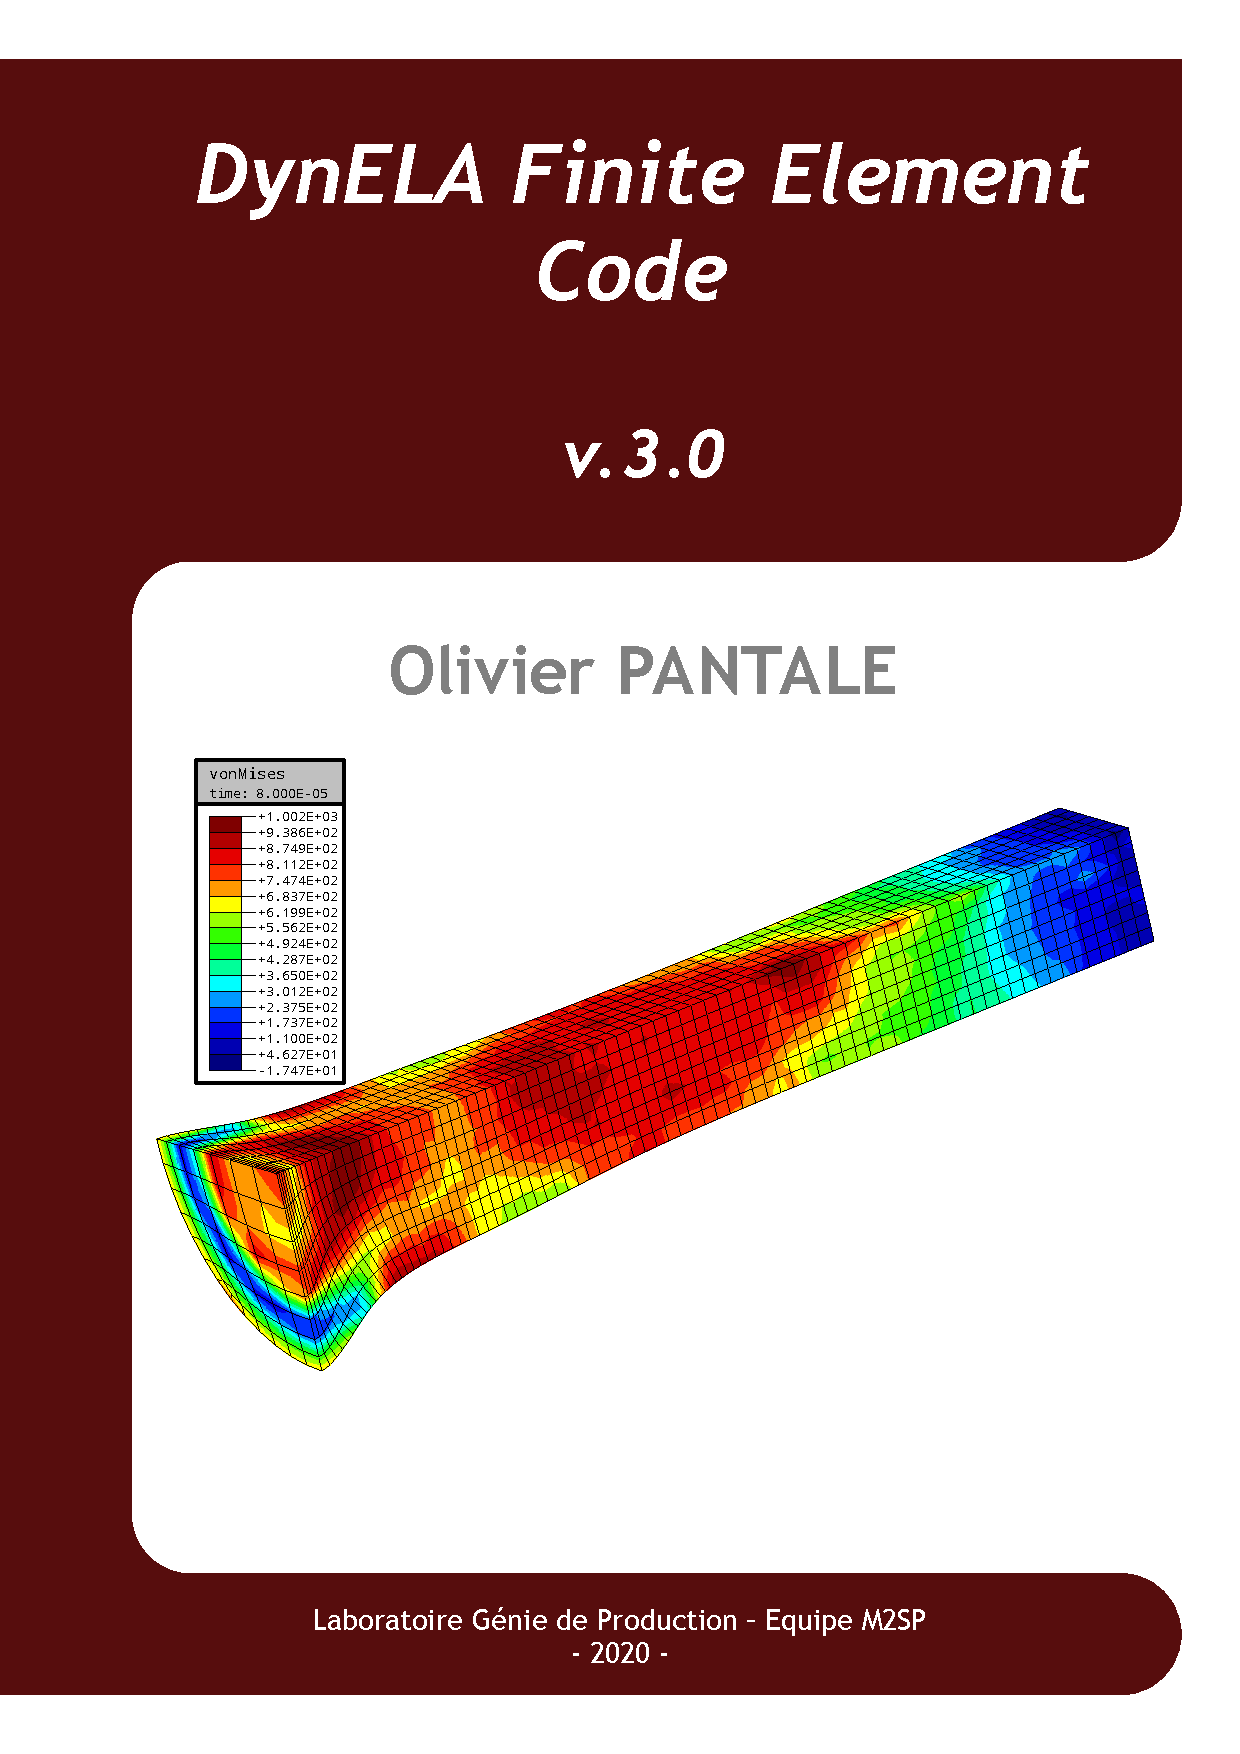
\includepdf[pages=1-2]{Cover.pdf}

\dominitoc\renewcommand{\thepage}{\roman{page}}\setcounter{page}{1}

% Includes Table of contents
\tableofcontents

% Includes List of Figures
\listoffigures

% Includes List of Tables
\listoftables

\cleardoublepage

\renewcommand{\thepage}{\arabic{page}}\setcounter{page}{1}

% !TeX spellcheck = en_US
% !TeX root = DynELA.tex
%
% LaTeX source file of DynELA FEM Code
%
% (c) by Olivier Pantalé 2020
%
\chapter*{Notations\addcontentsline{toc}{chapter}{Notations}\markboth{Notations}{Notations}}

\LETTRINE{F}rom a general point of view, it is usual to observe that one of the main difficulties in the field of mechanics, as in other fields, is the non-homogeneity of notations between the various authors. It is then easy to make completely incomprehensible the slightest theory when one decides to change notation. As the notion of universal notation is not yet valid (even if certain conventions can be assimilated to universal concepts), then we present below the set of notations used throughout this document and in a broader way in all the other documents in that series.

\subsection*{Notations Conventions \vspace{-1ex}}

\begin{longtable}[l]{>{\raggedright}p{0.2\paperwidth}>{\raggedright}p{0.8\paperwidth}}
$a$ & Scalar\tabularnewline
$\overrightarrow{a}$ & Vector\tabularnewline
$\A$ & $2^{nd}$ order Tensor or matrix\tabularnewline
$\IiA$ & $3^{rd}$ order Tensor\tabularnewline
$\IIA$ & $4^{th}$ order Tensor\tabularnewline
\end{longtable}

\subsection*{Linear Algebra and Mathematical Operators \vspace{-1ex}}

\begin{longtable}[l]{>{\raggedright}p{0.2\paperwidth}>{\raggedright}p{0.8\paperwidth}}
$\overrightarrow{a}\cdot\overrightarrow{b}$ & Dot product of the vectors $\overrightarrow{a}$ and $\overrightarrow{b}$\tabularnewline
$\overrightarrow{a}\otimes\overrightarrow{b}$ & Tensor (or Dyadic) product of the vectors $\overrightarrow{a}$ and $\overrightarrow{b}$\tabularnewline
$\overrightarrow{a}\wedge\overrightarrow{b}$ & Vectorial product of the vectors $\overrightarrow{a}$ and $\overrightarrow{b}$\tabularnewline
$\A:\B$ & Double contracted product of the two tensors $\A$ et $\B$\tabularnewline
$\stackrel{\bullet}{\boxempty}$ & Time derivative of quantity $\boxempty$\tabularnewline
$\stackrel{\bullet\bullet}{\boxempty}$ & Second order time derivative of quantity $\boxempty$\tabularnewline
$\boxempty_{,\boxempty}$ & Partial derivative of quantity $\boxempty$ with respect to $_{\boxempty}$\tabularnewline
$\boxempty^{T}$ & Transpose of a matrix or a vector $\boxempty$\tabularnewline
$\tr\,\boxempty$ & Trace of a matrix or a tensor $\boxempty$ ($\tr\,\boxempty=\sum\boxempty_{ii}$)\tabularnewline
$\dev\,\boxempty$ & Deviatoric part of a tensor $\boxempty$ ($\dev\,\boxempty=\boxempty-\frac{1}{3}\tr\,\boxempty \Id$)\tabularnewline
$\delta_{ij}$ & Kronecker delta identity\tabularnewline
$\Id$ & Unity matrix or second order tensor\tabularnewline
$\IId$ & Unity fourth order tensor\tabularnewline
\end{longtable}

\subsection*{Basic Continuum Mechanics\vspace{-1ex}}

\begin{longtable}[l]{>{\raggedright}p{0.2\paperwidth}>{\raggedright}p{0.8\paperwidth}}
$\overrightarrow{x}=\left[\begin{array}{ccc}
x & y & z\end{array}\right]^{T}$ & Coordinates in the physical domain\tabularnewline
$\overrightarrow{u}=\left[\begin{array}{ccc}
u & v & w\end{array}\right]^{T}$ & Displacement field\tabularnewline
$\overrightarrow{\omega}=\left[\begin{array}{ccc}
\omega_{x} & \omega_{y} & \omega_{z}\end{array}\right]^{T}$ & Rotation field\tabularnewline
$\Om$ & Arbitrary body in the current configuration\tabularnewline
$\Gam$ & Boundary of an arbitrary body $\Om$ in the current configuration\tabularnewline
$\rho$ & Material density\tabularnewline
$E$ & Young's modulus of a material\tabularnewline
$\nu$ & Poisson's ratio of a material\tabularnewline
$K$ & Bulk modulus of a material\tabularnewline
$\lambda$ & Lamé's first parameter of a material\tabularnewline
$\mu=G$ & Lamé's second parameter / Coulomb's shear modulus\tabularnewline
$\overrightarrow{F}$ & External load vector\tabularnewline
$\overrightarrow{f}$ & External load vector\tabularnewline
$\Eps$ & Green-Lagrange strain tensor\tabularnewline
$\Sig$ & Cauchy stress tensor\tabularnewline
$\Dev$ & Deviatoric part of the Cauchy stress tensor\tabularnewline
$\Alp$ & Backstress tensor\tabularnewline
$\Fi$ & $\Fi=\Dev-\Alp$\tabularnewline
\end{longtable}

\subsection*{Constitutive laws\vspace{-1ex}}

\begin{longtable}[l]{>{\raggedright}p{0.2\paperwidth}>{\raggedright}p{0.8\paperwidth}}
$f$ & \tabularnewline
$\n$ & Direction of the plastic flow\tabularnewline
$\q$ & Heredity variables in an elastoplastic behavior\tabularnewline
$\overline{\sigma}$ & von Mises equivalent stress\tabularnewline
$\overline{\varepsilon}^{p}$ & Equivalent plastic strain\tabularnewline
$\stackrel{\bullet}{\overline{\varepsilon}^{p}}$ & Equivalent plastic strain rate\tabularnewline
$\Lambda$ & Norm of the plastic strain\tabularnewline
$\sigma^{v}$ & \tabularnewline
$\sigma_{0}^{v}$ & \tabularnewline
$\sigma_{\infty}^{v}$ & \tabularnewline
\end{longtable}

\subsection*{Large Deformations\vspace{-1ex}}

\begin{longtable}[l]{>{\raggedright}p{0.2\paperwidth}>{\raggedright}p{0.8\paperwidth}}
$\overrightarrow{X}=\left[\begin{array}{ccc}
X & Y & Z\end{array}\right]^{T}$ & Coordinates in the reference domain\tabularnewline
$\E$ & Green-Lagrange deformation tensor\tabularnewline
$\F$ & Deformation gradient tensor\tabularnewline
$\U,\ \V$ & Right and left pure deformation tensors\tabularnewline
$\R$ & Rotation tensor\tabularnewline
$\iL$ & Deformation speed tensor\tabularnewline
$\D$ &Symmetric part of the $\iL$ tensor\tabularnewline
$\W$ & Skew-symmetric part of the $\iL$ tensor\tabularnewline
\end{longtable}

\subsection*{Finite Element Data Structures\vspace{-1ex}}
\begin{flushleft}
\begin{longtable}[l]{>{\raggedright}p{0.2\paperwidth}>{\raggedright}p{0.8\paperwidth}}
$\N$ &Shape functions matrix\tabularnewline
$\overrightarrow{\xi}=\left[\begin{array}{ccc}
\xi & \eta & \zeta\end{array}\right]^{T}$ & Coordinates in the parent domain\tabularnewline
$\B$ & Derivatives of the shape functions\tabularnewline
$\boxempty^{e}$ & Quantity $\boxempty$ related to element $e$\tabularnewline
$\J$ & Jacobian matrix\tabularnewline
$\M$ & Mass matrix\tabularnewline
$\K$ & Stiffness matrix\tabularnewline
$\overline{\F}$ & External surfacic load vector\tabularnewline
$\F$ & External load vector\tabularnewline
$\overline{\f}$ & External volumic load vector\tabularnewline
$\q$ & Nodal unknowns vector\tabularnewline
$n_{g}$ & Number of nodes of the current element\tabularnewline
$n_{Q}$ & Number of integration points of the current element\tabularnewline
\end{longtable}
\par\end{flushleft}



% !TeX spellcheck = en_US
% !TeX root = DynELA.tex
%
% LaTeX source file of DynELA FEM Code
%
% (c) by Olivier Pantalé 2020
%
\chapter{Installation of the \DynELA}\label{Chapter!Installation}

\startcontents[chapters]
\printmyminitoc[1]\LETTRINE{T}he \DynELA is an Explicit FEM code written in \Cpp using a Python's interface for creating the Finite Element Models. This is a new version of the early proposed v.2 code written between 1996 and 2010. The aim of v.4.0 is to provide an enhanced version of the code with enhancements concerning the constitutive laws, a new programming interface based on Python 3 formalism, along with some enhanced documentation.
The \DynELA is developed under Linux (an ubuntu 20.04 LTS is currently used for the development). All source code and material can be downloaded from the following gitlab
%or github
 website
%s
:

\hspace*{1cm}\textsf{https://git.enit.fr/opantale/dynela-v.-4.0.git}
%  \hspace*{1cm}\textsf{https://github.com/pantale/DynELA}

The \DynELA is licensed under BSD-3-Clause license \footnote{See sources of information on Internet if you don't know what it means.}.

\section{Prerequisites}

Compilation of the \DynELA requires several libraries.
Generation of Makefiles for the compilation of the \DynELA is based on the use of the CMake tool. CMake is a cross-platform, open-source build system generator. Under ubuntu it can be installed with the following command:

\begin{BashListing}[numbers=none]
sudo apt install cmake
\end{BashListing}

DynELA is written in \Cpp and Python 3 therefore it needs a \Cpp compiler and some Python 3 libraries. Under ubuntu those libraries can be installed with the following command:

\begin{BashListing}[numbers=none]
sudo apt install build-essential swig zlib1g-dev liblapacke-dev python3-dev
\end{BashListing}

It also needs some Python 3 modules to run properly and at least numpy and matplotlib:

\begin{BashListing}[numbers=none]
sudo apt install python3-numpy python3-matplotlib texlive dvipng \
texlive-latex-extra texlive-fonts-recommended
\end{BashListing}

\section{Download and compilation}

Downloading of the source code from the github repository\footnote{Here, we consider that the software is available from the ENIT gitlab repository at the following address: https://git.enit.fr/opantale/dynela-v.-4.0.git. You can adapt the proposed installation procedure if it is not your case.}, compilation and installation of the software into a sub-directory named \textsf{DynELA} can be done using the following procedure:

\begin{BashListing}[numbers=none]
git clone https://git.enit.fr/opantale/dynela-v.-4.0.git DynELA
cd DynELA
mkdir Build
cd Build
cmake ../Sources
make
\end{BashListing}

After downloading and compilation, there is no need to install the executable or something similar to use the FEM code. You just have to modify the \textsf{.bashrc} file and add the following lines where \emph{path\_to\_DynELA} points to the top directory of your \DynELA installation:

\begin{BashListing}[numbers=none]
export DYNELA="path_to_DynELA"
export PATH=$PATH:$DYNELA/bin
export DYNELA_BIN=$DYNELA/Build/bin
export DYNELA_LIB=$DYNELA/Build/lib
export PYTHONPATH="$DYNELA_BIN:$PYTHONPATH"
export PYTHONPATH="$DYNELA_LIB:$PYTHONPATH"
export LD_LIBRARY_PATH=$DYNELA_LIB:$LD_LIBRARY_PATH
\end{BashListing}

Of course, you have to execute \textsf{source .bashrc} to take into account those modifications, or launch another terminal.

\section{Testing and usage}

Testing of the installation can be done by running one of the provided samples. All samples of the \DynELA are located into the sub-directories of the Samples folder. Running a simulation is done using the following command in one of the Samples sub-directories:

\begin{BashListing}[numbers=none]
python sample.py
\end{BashListing}

Running the tests in the Samples directories can also be done with regard to the Makefiles contained in the Samples directories. Benchmark tests can be run from any sub-directory of the Sample folder using the following command:

\begin{BashListing}[numbers=none]
make
\end{BashListing}

The \DynELA now has a class for direct export of contourplot results using SVG vectorial format for a 2D or 3D mesh and time-history curves through the Python command interface. See the documentation for all instructions concerning SVG and time-history outputs and the examples included in the Samples directories.

The DynELA FEM code can generate VTK files for the results. The Paraview postprocessor can be used to visualize those results. Paraview is available here:

\hspace*{1cm}\textsf{\hspace*{1cm}\textsf{https://www.paraview.org}}

Refer to the documentation of the ParaView software to know how to install it, and use it. This is out of scope from this documentation.


\part{DynELA FEM code theory}

% !TeX spellcheck = en_US
% !TeX root = DynELA.tex
%
% LaTeX source file of DynELA FEM Code
%
% (c) by Olivier Pantalé 2020
%
\chapter{Theory}

\startcontents[chapters]
\printmyminitoc[1]\LETTRINE{T}he \DynELA is an Explicit FEM code written in \Cpp using a Python's interface for creating the Finite Element Models. 

\section{Introduction}

\begin{tcolorbox}[width=0.95\textwidth,myTab,tabularx={l||C|C|C|C|C},title=Homogeneous system of units in mechanics]%,boxrule=0.5pt]
              & Dimension        & SI (MKS)   & SI (mm-s)  & SI (mm-kg)  & SI (mm-kg-s) \\\hline\hline
Length        & $L$              & $m$        & $mm$       & $mm$        & $mm$        \\\hline
Weight        & $M$              & $kg$       & $T$        & $kg$        & $kg$        \\\hline
Time          & $T$              & $s$        & $s$        & $ms$        & $s$         \\\hline
Stress        & $ML^{-1}T^{-2}$  & $Pa$       & $MPa$      & $GPa$       & $kPa$       \\\hline
Force         & $MLT^{-2}$       & $N$        & $N$        & $kN$        & $mN$        \\\hline
Energy        & $ML^{2}T^{-2}$   & $J$        & $mJ$       & $J$         & $MJ$        \\\hline
Density       & $ML^{-3}$        & $kg/m^{3}$ & $T/mm^{3}$ & $kg/mm^{3}$ & $kg/mm^{3}$ \\\hline
Speed         & $LT^{-1}$        & $m/s$      & $mm/s$     & $mm/ms$     & $mm/s$      \\\hline
Angular speed & $T^{-1}$         & $s^{-1}$   & $s^{-1}$   & $ms^{-1}$   & $s^{-1}$    \\\hline
Acceleration  & $LT^{-2}$        & $m/s^{2}$  & $mm/s^{2}$ & $mm/ms^{2}$ & $mm/s^{2}$  \\\hline
Couple        & $ML^{2}T^{-2}$   & $N.m$      & $N.mm$     & $kN.mm$     & $mN.mm$
\end{tcolorbox}


\cleardoublepage

\part{DynELA Programming}

% !TeX spellcheck = en_US
% !TeX root = DynELA.tex
%
% LaTeX source file of DynELA FEM Code
%
% (c) by Olivier Pantalé 2020
%
\chapter{DynELA programming language}

\startcontents[chapters]
\printmyminitoc[2]\LETTRINE{T}his chapter deals about the \DynELA programming language. This language is based on Python 3 and all models must be described using this formalism. Therefore, this chapter will describe step by step how to build a Finite Element Model for the \DynELA, using the Python 3 language. To set-up a model in DynELA, a good knowledge of the Python's 3 language is not mandatory, but it will help to be skillful concerning this language. On the other hand advanced features can be setup with the help of Python 3 language.

\section{Introduction and basic knowledge}
The Python 3 language serves as a support for describing FEM in DynELA. Construction of the Finite Element Model is done by calling some \Cpp~methods of the DynELA library through Python language. In fact, the \Cpp~methods of the DynELA library are encapsulated by the help of SWIG. Some methods of the DynELA library have therefore been encapsulated using the SWIG utility and are directly accessible from the Python language.

\subsection{Calling the python interpreter}

After the installation and compilation phase of the code\footnote{See the installation instructions in chapter \ref{Chapter!Installation} of the preamble, page \pageref{Chapter!Installation}}, the \DynELA can be used using the following command:

\begin{BashListing}
python model.py
\end{BashListing}

where \textsf{model.py} is the Python 3 source file defining the Finite Element Model. The \textsf{model.py} file contains the definition of the Finite Element Model using a Python 3 language and calls to specific DynELA methods written in \Cpp. The formalism used to set up this Python source file are described is the subsequent chapters.

\subsection{Formalism of a DynELA python file}

To build a Finite Element Model, it is mandatory to import the \textsf{dnlPython} interpreter from the \textsf{.py} script. Conforming to this formalism, we give hereafter the minimal piece of Python code to set up a Finite Element Model in the \DynELA.\index[PL]{dnlPython}

\begin{PythonListing}
#!/usr/bin/env python3
import dnlPython as dnl # Imports the dnlPython library as dnl
model = dnl.DynELA()    # Creates the main Object
...                     # Set of instructions to build the FE model
...                     # conforming to the DynELA language and Python 3
model.solve()           # Runs the solver
...                     # Set of instructions to postprocess the FE model
\end{PythonListing}

In the preceding piece of code, line 2 is used to load into the namespace \textsf{dnl} the \textsf{dnlPython} module containing the interface to all \Cpp~methods of the \DynELA, based on the use of the SWIG Python interface. Of course, and conforming to the \textsf{import} command, any name can be used as a namespace to import the DynELA top library. Therefore, all public methods of the \DynELA written in \Cpp~can be called from the Python script to build the Finite Element Model, launch the solver, produce output results,\ldots

In the proposed piece of code, line 3 is used to create an object of type \textsf{DynELA} (the higher object type in the \DynELA library) and instantiate it as the \textsf{model} object\footnote{For the rest of this chapter, we assume that the name of the instantiated \textsf{DynELA} object is \textsf{model}.}, while line 6, the solver of the \DynELA library is called to solve the problem and produce the results.

It is also possible, but not recommended, to use the following syntax for lines 2 and 3 of the previous block:
\begin{PythonListing}
#!/usr/bin/env python3
from dnlPython import * # Imports the dnlPython library in current namespace
model = DynELA()        # Creates the main Object
...                     # Rest of the source code defining the FE model
\end{PythonListing}
and then access all top methods and object of the DynELA library directly without referring to the namespace, such as what is proposed in line 3 of the previous block.

As the interpreter of the \DynELA is based on Python 3 language, we can use all instructions valid in Python 3 along with the specific DynELA instructions. In the rest of this documentation, we assume that the notions of programming in Python are mastered, and we will focus only on the functions specific to the \DynELA.


\section{Model, Nodes and Elements}

All Finite Element Models involves nodes and elements. The very first part of the model is therefore to create the nodes and the elements of the structure to set up a Finite Element Model. The \DynELA library doesn't include any meshing procedure yet, therefore, it is mandatory to create all elements and all nodes by hand or using Python loops in case it can be used.

Another way is to use an external meshing program and convert the output of this program to produce the ad hoc lines of Python to describe the elements and the nodes of the model. This has been used many times by the author, and the Abaqus Finite Element code is an efficient way to create the mesh using the \textsf{.inp} text file generated by the CAE Abaqus program and then convert the nodes and elements description parts of the Abaqus inp file into DynELA formalism.

\subsection{Model}

Definition of a model in the \DynELA is done by creating an instance of the \textsf{DynELA} object into memory. This is done by calling the \textsf{dnlPython.DynELA(string)} method that returns an object of type \textsf{DynELA} as presented hereafter.\index[PL]{dnlPython!DynELA(string)}

\begin{PythonListing}
import dnlPython as dnl       # Imports the dnlPython library as dnl
model = dnl.DynELA('Taylor')  # Creates the main Object model named Taylor
\end{PythonListing}

In line 2 of the preceding piece of code, a reference name\footnote{The reference name is a string used to identify the object, this is completely optional but useful for debugging purposes for example as one can know the associated name to an object.} \textsf{Taylor} is associated to the \textsf{model} object during creation. Once the model is created, one can then define all nodes, elements, materials, constitutive laws, boundary conditions,\ldots

\subsection{Nodes}

\subsubsection{Definition of the nodes}

In the \DynELA, creation of nodes is done by calling the \textsf{DynELA::createNode()} method. Therefore, a node is created by calling the \textsf{createNode()} method and giving the new node number and the $x$, $y$ and $z$ coordinates of the new node as presented just below.\index[PL]{DynELA!createNode(int, float, float, float)}

\begin{PythonListing}
model.createNode(1, 0.0, 0.0, 0.0)  # Creates node 1, coordinates [0.0, 0.0, 0.0]
model.createNode(2, 1.0, 2.0, -1.0) # Creates node 2, coordinates [1.0, 2.0, -1.0]
\end{PythonListing}

An alternative method can be used if the coordinates of the node are already stored into a Vec3D object as presented hereafter.\index[PL]{DynELA!createNode(int, Vec3D)}

\begin{PythonListing}
vect = dnl.Vec3D(1.0, 2.0, -1.0) # Creates a Vec3D object [1.0, 2.0, -1.0]
model.createNode(1, vect)        # Creates node 1 with coordinates vect
\end{PythonListing}

A check of the total number of nodes of the structure can be done using the \textsf{DynELA.getNodesNumber()} method that returns the total number of nodes created.

\subsubsection{Definition of the Nodes sets}

Manipulation of nodes, application of boundaries conditions, etc,\ldots is done through the definition of nodes sets. Such nodes sets are used to group nodes under a \textsf{NodeSet} object for further use. A \textsf{NodeSet} object contains a reference name and a list of nodes. Creation of a \textsf{NodeSet} is done using the \textsf{DynELA.NodeSet()} method that returns an new \textsf{NodeSet} instance. The \textsf{NodeSet} can be named during the creation by specifying its name as a string.\index[PL]{NodeSet(string)}

\begin{PythonListing}
nset = dnl.NodeSet('NS_All')
\end{PythonListing}

When the \textsf{NodeSet} has been created, one can now define the list of nodes constituting the \textsf{NodeSet} with the generic \textsf{DynELA.add()} method with the following formalism:

\textsf{DynELA.add(nodeset, start, end, increment)}

Hereafter is some self explaining examples to illustrate this process.

\begin{PythonListing}
nset = dnl.NodeSet('NS_All')
model.add(nset, 2)       # Add node number 2 to node set
model.add(nset, 1, 4)    # Add nodes number 1-4 to node set
model.add(nset, 1, 4, 2) # Add nodes number 1 and 3 to node set
\end{PythonListing}

\subsection{Elements}

\subsubsection{Definition of the elements}

Creation of elements is done by calling the \textsf{DynELA.createElement()} method. An element is created by calling the \textsf{createNode()} method and giving the new element number and the list of nodes defining the element shape separated by comas and ordered thanks to the element definition as presented just hereafter.

\textsf{DynELA.createElement(elementNumber, node1, node2,\ldots)}

Before creating the very first element of the structure, it is necessary to define the element shape using the \textsf{DynELA.setDefaultElement()} method. An example of element creation combining the two preceding methods is presented hereafter.\index[PL]{DynELA!setDefaultElement(Element)}\index[PL]{DynELA!createElement(int, int, int,...)}

\begin{PythonListing}
model.setDefaultElement(dnl.Element.ElQua4N2D) # Defines the default element
model.createElement(1, 1, 2, 3, 4)             # Creates element 1 with nodes 1,2,3,4
\end{PythonListing}

The following elements are available in the \DynELA.
\begin{description}
\item [ElQua4n2D]: 4 nodes bi-linear 2D quadrilateral element.
\item [ElQua4NAx]: 4 nodes bi-linear axisymmetric quadrilateral element.
\item [ElTri3N2D]: 3 nodes 2D triangular element.
\item [ElHex8N3D]: 8 nodes 3D hexahedral element.
\item [ElTet4N3D]: 4 nodes 3D tetrahedral element.
\item [ElTet10N3D]: 10 nodes 3D tetrahedral element.
\end{description}
The total number of elements of the structure can be checked using the \textsf{DynELA.getElementsNumber()} method that returns the total number of elements created.

\subsubsection{Definition of the Element sets}

Declaration of materials, boundaries conditions, etc\ldots is done through the definition of elements sets. Such elements sets are used to group elements under an \textsf{ElementSet} object for further use. An \textsf{ElementSet} object contains a reference to a name and a list of elements. Creation of an \textsf{ElementSet} is done using the \textsf{DynELA.ElementSet()} method that returns a new \textsf{ElementSet} instance. The \textsf{ElementSet} can be named during the creation by specifying its name as a string.

\begin{PythonListing}
eset = dnl.ElementSet('ES_All')
\end{PythonListing}

When the \textsf{ElementSet} has been created, one can now define the list of elements constituting the \textsf{ElementSet} with the generic \textsf{DynELA.add()} method according to the following formalism:

\textsf{DynELA.add(elementset, start, end, increment)}

Hereafter is some self explaining examples to illustrate this process.

\begin{PythonListing}
eset = dnl.ElementSet('ES_All')
model.add(eset, 2)       # Add element number 2 to element set
model.add(eset, 1, 4)    # Add elements number 1-4 to element set
model.add(eset, 1, 4, 2) # Add elements number 1 and 3 to element set
\end{PythonListing}

\subsection{Coordinates transformations}

When the mesh has been created, it is always possible to modify the geometry of the structure by applying some geometrical operations such as translations, rotations and change of scale. Those operations apply on a \textsf{NodeSet}.

\subsubsection{Translations}

One can define a translation of the whole model or a part of the model by defining a translation vector (an instance of the \DynELA \textsf{Vec3D}) and apply this translation to the whole structure (without specifying the \textsf{NodeSet}) or a \textsf{NodeSet} using the \textsf{DynELA.translate()} method with the following syntax.

\begin{PythonListing}
vector = dnl.Vec3D(1, 0, 0)   # Defines the translation vector
model.translate(vector)       # Translates the whole model along [1, 0, 0]
model.translate(vector, nset) # Translates the NodeSet nset along [1, 0, 0]
\end{PythonListing}

\subsubsection{Rotations}

One can define a rotation of the whole model or a part of the model by defining a rotation vector (global axes $\overrightarrow{\ensuremath{x}}$, $\overrightarrow{y}$, $\overrightarrow{\ensuremath{z}}$ or an instance of the \DynELA \textsf{Vec3D}) and an angle $\alpha$ then apply this rotation to the whole structure (without specifying the \textsf{NodeSet}) or a \textsf{NodeSet} using the \textsf{DynELA.rotate()} method with the following syntax.

\begin{PythonListing}
model.rotate('X', angle)        # Rotation of the whole structure around X
model.rotate('X', angle, nset)  # Rotation of NodeSet nset around X
axis = dnl.Vec3D(1.0, 1.0, 1.0) # Defines the axis of rotation
model.rotate(axis, angle)       # Rotation of the whole structure around axis
model.rotate(axis, angle, nset) # Rotation of NodeSet nset around axis
\end{PythonListing}

\subsubsection{Scaling}

One can define a scaling of the whole model or a part of the model by defining a scale factor or a scale vector (an instance of the \DynELA \textsf{Vec3D}) and apply this scaling operation to the whole structure (without specifying the \textsf{NodeSet}) or a \textsf{NodeSet} using the \textsf{DynELA.scale()} method with the following syntax.

\begin{PythonListing}
model.scale(value)             # Scales the whole structure by factor value
model.scale(value, nset        # Scales the NodeSet nset by factor value
vec = dnl.Vec3D(2.0, 1.0, 1.0) # Defines the scale vector
model.scale(vec)               # Scales the whole structure by a factor of 2.0 on x
model.scale(vec, nset)         # Scales the NodeSet nset by a factor of 2.0 on x
\end{PythonListing}

\section{Materials}

\subsection{Declaration of materials}

\subsubsection{Material declaration}

Creation of a Material is done using the \textsf{DynELA.Material()} method. It is possible to give a name to a material during the creation process by specifying it through a string during the declaration. This can be used further.

\begin{PythonListing}
# Creates the material
steel = dnl.Material('Steel')
\end{PythonListing}

\subsubsection{General properties of materials}

General properties of materials in \DynELA concerns the general constants such as Young's modulus, Poisson's ratio, density,\ldots The complete list of parameters is reported in Table \ref{tab:Programming!GeneralProperties}.
\begin{table}[h]
	\begin{center}\begin{tcolorbox}[width=.75\textwidth,myTab,tabularx={l|c|c|R}]
			\multicolumn{1}{c|}{Name} & Symbol & Unit & \multicolumn{1}{c}{Description} \\ \hline\hline
			youngModulus & $E$ & $MPa$ & Young modulus\\
			poissonRatio & $\nu$ &  & Poisson ratio\\
			density & $\rho$ & $kg/m^3$ & Density\\
			heatCapacity & $C_{p}$ & $J/^{\circ}C$ & Heat capacity\\
			taylorQuinney& $\eta$ & & Taylor-Quinney coefficient\\
			initialTemperature & $T_{0}$ & $^{\circ}C$ & Initial temperature
	\end{tcolorbox}\end{center}\caption{General properties of materials\label{tab:Programming!GeneralProperties}}
\end{table}
After creating an instance of the object \textsf{dnl.Material}, on can apply the prescribed values to all those parameters using the following syntax.

\begin{PythonListing}
# Creates the material
steel = dnl.Material('Steel')
# Apply all parameters
steel.youngModulus = 206e9
steel.poissonRatio = 0.3
steel.density = 7830
steel.heatCapacity = 46
steel.taylorQuinney = 0.9
steel.initialTemperature = 25
\end{PythonListing}

\subsubsection{Material affectation to a set of elements}

And, the material can be affected to the elements of the model by the \textsf{DynELA.add()} method as proposed hereafter.

\begin{PythonListing}
# Creates the material
steel = dnl.Material('Steel')
# Apply all parameters
...
# Affect the material to the element set eset
model.add(steel, eset)
\end{PythonListing}

\subsection{Johnson-Cook constitutive law}

The Johnson-Cook constitutive law is an hardening law defining the yield stress $\sigma^{y}(\overline{\varepsilon}^{p},\stackrel{\bullet}{\overline{\varepsilon}^{p}},T)$ by the following equation:

\begin{equation}
\sigma^{y}=\left(A+B\overline{\varepsilon}^{p^{n}}\right)\left[1+C\ln\left(\frac{\stackrel{\bullet}{\overline{\varepsilon}^{p}}}{\stackrel{\bullet}{\overline{\varepsilon}_{0}}}\right)\right]\left[1-\left(\frac{T-T_{0}}{T_{m}-T_{0}}\right)^{m}\right]
\end{equation}
where $\stackrel{\bullet}{\overline{\varepsilon}_{0}}$ is the reference strain rate, $T_{0}$ and $T_{m}$ are the reference temperature and the melting temperature of the material respectively and $A$, $B$, $C$, $n$ and $m$ are the five constitutive flow law parameters. Therefore, this kind of hardening law can be defined by using the following piece of code:

\begin{PythonListing}
hardLaw = dnl.JohnsonCookLaw()                       # Hardening law
hardLaw.setParameters(A, B, C, n, m, depsp0, Tm, T0) # Parameters of the law
\end{PythonListing}

Once the hardening law has been created, one have to link this hardening law to a material already defined using the following piece of code:

\begin{PythonListing}
# Creates the material
steel = dnl.Material('Steel')
# Creates the hardening law
hardLaw = dnl.JohnsonCookLaw()
# Attach hardening law to material
steel.setHardeningLaw(hardLaw)
\end{PythonListing}

\section{Boundaries conditions}

\subsection{Restrain boundary condition}

\begin{PythonListing}
# Declaration of a boundary condition for top part
topBC = dnl.BoundaryRestrain('BC_top')
topBC.setValue(0, 1, 1)
model.attachConstantBC(topBC, topNS)
\end{PythonListing}

\subsection{Amplitude}

\begin{PythonListing}
# Declaration of a ramp function to apply the load
ramp = dnl.RampFunction('constantFunction')
ramp.set(dnl.RampFunction.Constant, 0, stopTime)
\end{PythonListing}

\subsection{Constant speed}

\begin{PythonListing}
# Declaration of a boundary condition for top part
topSpeed = dnl.BoundarySpeed()
topSpeed.setValue(displacement, 0, 0)
topSpeed.setFunction(ramp)
model.attachConstantBC(topSpeed, topNS)
\end{PythonListing}

\subsection{Initial speed}

\begin{PythonListing}
# Declaration of a ramp function to apply the load
ramp = dnl.RampFunction('constantFunction')
ramp.set(dnl.RampFunction.Constant, 0, stopTime)
\end{PythonListing}

\section{Fields}\label{ProgrammingLanguage:Section:Fields}

\subsection{Nodal fields}

Nodal fields are defined at nodes and cover types defined in table \ref{tab:Programming!NodalFields}. Concerning those fields, some of them are directely defined at nodes, some other are extrapolated from integration points and transfered to nodes as reported in column \textsf{loc} of table \ref{tab:Programming!NodalFields}. Concerning types, \textsf{scalars}, \textsf{vec3D} and \textsf{tensors} are available. Depending in the type of data, different methods can be used to acces those data:
\begin{description}
	\item [{scalar}] : Direct access to the value as it is unique.
	\item [{vec3D}] : Access to all $3$ components of a vec3D using \textsf{nameX}, \textsf{nameY}, \textsf{nameZ} or the norm of the vec3D using \textsf{name}.
	\item [{tensor}] : Access to all $9$ components of a tensor using \textsf{nameXX}, \textsf{nameXY},\ldots, \textsf{nameZZ} or the norm of the tensor using \textsf{name}.
\end{description}
\begin{table}[h]
	\begin{center}\begin{tcolorbox}[width=.85\textwidth,myTab,tabularx={l|c|c|c|c|R}]
			\multicolumn{1}{c|}{Name} & & Type & nb & Loc & \multicolumn{1}{c}{Description} \\ \hline\hline
			density & $\rho$ & scalar & $1$ & IntPt &\\ \hline
			displacementIncrement & $\Delta\overrightarrow{u}$ & vec3D & $3+1$ & node & \\ \hline
			displacement & $\overrightarrow{u}$ & vec3D & $3+1$ & node & \\ \hline
			energyIncrement && scalar & $1$ & IntPt & \\ \hline
			energy && scalar & $1$ & IntPt & \\ \hline
			gammaCumulate && scalar & $1$ & IntPt & \\ \hline
			gamma & $\Gamma$ & scalar & $1$ & IntPt & \\ \hline
			internalEnergy && scalar & $1$ & IntPt & \\ \hline
			mass & $m$ & scalar & $1$ & node & \\ \hline
			nodeCoordinate & $\overrightarrow{x}$ & vec3D & $3+1$ & node & \\ \hline
			normal & $\overrightarrow{n}$ & vec3D & $3+1$ & node & \\ \hline
			PlasticStrainInc && tensor & $9+1$ & IntPt & \\ \hline
			plasticStrainRate && scalar & $1$ & IntPt & \\ \hline
			plasticStrain && scalar & $1$ & IntPt & \\ \hline
			PlasticStrain && tensor & $9+1$ & IntPt & \\ \hline
			pressure & $p$ & scalar & $1$ & IntPt & \\ \hline
			speedIncrement & $\Delta\overrightarrow{v}$ & vec3D & $3+1$ & node & \\ \hline
			speed & $\overrightarrow{v}$ & vec3D & & node & \\ \hline
			StrainInc && tensor & $9+1$ & IntPt & \\ \hline
			Strain && tensor & $9+1$ & IntPt & \\ \hline
			Stress & $\Sig$ & tensor & $9+1$ & IntPt & \\ \hline
			temperature & $T$ & scalar & $1$ & IntPt & \\ \hline
			vonMises & $\overline{\sigma}$ & scalar & $1$ & IntPt & \\ \hline
			yieldStress & $\sigma^y$ & scalar & $1$ & IntPt &
	\end{tcolorbox}\end{center}\caption{Nodal fields\label{tab:Programming!NodalFields}}
\end{table}

\subsection{Element fields}

Element fields are defined at integration points and cover types defined in table \ref{tab:Programming!ElementlFields}. Concerning types, \textsf{scalars}, \textsf{vec3D} and \textsf{tensors} are available. Depending in the type of data, different methods can be used to acces those data:
\begin{description}
	\item [{scalar}] : Direct access to the value as it is unique.
	\item [{vec3D}] : Access to all $3$ components of a vec3D using \textsf{nameX}, \textsf{nameY}, \textsf{nameZ} or the norm of the vec3D using \textsf{name}.
	\item [{tensor}] : Access to all $9$ components of a tensor using \textsf{nameXX}, \textsf{nameXY},\ldots, \textsf{nameZZ} or the norm of the tensor using \textsf{name}.
\end{description}
\begin{table}[h]
	\begin{center}\begin{tcolorbox}[width=.85\textwidth,myTab,tabularx={l|c|c|c|R}]
			\multicolumn{1}{c|}{Name} && Type & nb & \multicolumn{1}{c}{Description} \\ \hline\hline
			density & $\rho$ & scalar & $1$ & \\ \hline
			gammaCumulate && scalar & $1$ & \\ \hline
			gamma & $\Gamma$ & scalar & $1$ & \\ \hline
			internalEnergy && scalar & $1$ & \\ \hline
			plasticStrainRate && scalar & $1$ & \\ \hline
			plasticStrain && scalar & $1$ & \\ \hline
			PlasticStrain && tensor & $9+1$ & \\ \hline
			PlaticStrainInc && tensor & $9+1$ & \\ \hline
			pressure & $p$ & scalar & $1$ & \\ \hline
			StrainInc && tensor & $9+1$ & \\ \hline
			Strain && tensor & $9+1$ & \\ \hline
			Stress & $\Sig$ & tensor & $9+1$ & \\ \hline
			temperature & $T$ & scalar & $1$ & \\ \hline
			vonMises & $\overline{\sigma}$ & scalar & $1$ & \\ \hline
			yieldStress & $\sigma^y$ & scalar & $1$ &
	\end{tcolorbox}\end{center}\caption{Element fields\label{tab:Programming!ElementlFields}}
\end{table}

\subsection{Global fields}

\begin{table}[h]
	\begin{center}\begin{tcolorbox}[width=.85\textwidth,myTab,tabularx={l|c|c|c|R}]
			\multicolumn{1}{c|}{Name} && Type & nb & \multicolumn{1}{c}{Description} \\ \hline\hline
			kineticEnergy & $E_c$ & scalar & $1$ & \\ \hline
			realTimeStep & $\Delta t_r$ & scalar & $1$ & \\ \hline
			timeStep &$\Delta t$& scalar & $1$ &
	\end{tcolorbox}\end{center}\caption{Global fields\label{tab:Programming!GlobalFields}}
\end{table}

\section{Data Output during computation}

\subsection{VTK Data files}
The \DynELA is able to export results in VTK (The Visualization Toolkit\footnote{See : https://vtk.org}) ASCII files. Those files can be used to visualize the results of computations using the Paraview post-processing software\footnote{See : https://www.paraview.org}.

Those VTK files are automatically created during the solving phase. Controlling the instant of file save is done using the following syntax:\index[PL]{DynELA!setSaveTimes(float, float, float)}
\begin{PythonListing}
model.setSaveTimes(startTime, stopTime, incrementTime)
\end{PythonListing}
where \textsf{startTime}, \textsf{stopTime}, \textsf{incrementTime} are $3$ times defining respectively the times of the first file, the last one and the period of time between subsequent frames.

At any time, it is possible to export a VTK file using the method \textsf{writeVTKFile( )}\index[PL]{DynELA!writeVTKFile( )} of the \textsf{DynELA} class.

\subsection{History files}

During the solving procedure, one can export time history datafiles that can be used to produce time-history plots. This kind of files are text files in CSV format directly exported from the DynELA solver. In order to control the production of those files, one have to create an instance of the \textsf{HistoryFile} class and add this instance to the current model. Those history-files can then be used to produce high-quality plots through the associated \textsf{Curves Utility} of the \DynELA presented in chapter \ref{chap:CU!CU}, or use the produced data-file in any external plotting application.

As an illustration, the following commented piece of code has been used to produce the CSV history file reported in Figure \ref{fig:PL!HF!Export}.
\begin{PythonListing}
hist = dnl.HistoryFile()              # Constructor of the hist object
hist.setFileName('HistoryPlot.plot')  # Sets the filename of the history file
hist.add(dnl.Field.timeStep)                 # First column will be timeStep value
hist.add(histES, 0, dnl.Field.vonMises)      # Second one will be von Mises stress
hist.add(histRad, dnl.Field.nodeCoordinateX) # Third one will be X node coordinate
hist.setSaveTime(1e-6)                       # One data every 1E-6 s
model.add(hist)                              # Add the time history to the solver
\end{PythonListing}

\begin{figure}[h]
\begin{centering}
\begin{BashListing}
#DynELA FEM Code v. 4.0 history file
#plotted :timeStep vonMises nodeCoordinateX
0.0000000E+00 6.2463483E-08 0.0000000E+00 3.2000000E+00
1.0623148E-06 6.2462797E-08 1.3439840E+03 3.5412151E+00
2.0617159E-06 6.2462515E-08 1.3643205E+03 3.7516529E+00
3.0611173E-06 6.2462676E-08 1.3748692E+03 3.9635932E+00
4.0605220E-06 6.2462901E-08 1.3662499E+03 4.1161636E+00
5.0599347E-06 6.2465035E-08 1.3539346E+03 4.2812566E+00
.....
\end{BashListing}
\par\end{centering}
\caption{Export of a CSV history file\label{fig:PL!HF!Export}}
\end{figure}

In file reported in Figure \ref{fig:PL!HF!Export}, the first two lines are comments. Line $1$ shows the name and version of the \DynELA while line $2$ shows the name of the fields from columns 2 to the end of the table (in this example, current time is in column 1, time-step $\Delta t$ is in column 2, von Mises stress $\overline{\sigma}$ at the center of the element referred by element-set \emph{histES} is in column 3 and nodal coordinate $x$ of the node defined in \emph{histRad} node-set is in the last column of the table). One data is more or less produced at each requested time ($t_i=10^{-6}s$), but this depends on the time-step increment $\Delta t$ of the Explicit solver.

\subsubsection{Definition of data to save}

\begin{description}
\item [{add (\emph{ElementSet}, \emph{int}, \emph{field})}] : Add the output data \emph{field} defined at integration point \emph{int} for all elements defined in the element-set \emph{ElemenSet} to the current time-history plot.\index[PL]{HistoryFile!add(ElementSet)}
\item [{add (\emph{NodeSet}, \emph{Field})}] : Add the output data \emph{Field} for all nodes defined in the node-set \emph{NodeSet} to the current time-history plot.\index[PL]{HistoryFile!add(NodeSet)}
\item [{add (\emph{Field})}] : Add the global \emph{Field} value to the current time-history plot.\index[PL]{HistoryFile!add(Field)}
\item [{setFileName (\emph{string})}] : Defines the name of the output CSV filename.\index[PL]{HistoryFile!setFileName(string)}
\item [{setSaveTime (\emph{float})}] : Defines the frequency of data store during the computation.\index[PL]{HistoryFile!setSaveTime(float)}
\item [{setSaveTime (\emph{float}[start], \emph{float}[stop], \emph{float}[freq])}] : Defines the start, stop and frequency of data store during the computation starting at \emph{start}, ending at \emph{stop} and with the frequency defined by \emph{freq}.\index[PL]{HistoryFile!setSaveTime(float, float, float)}
\end{description}

When data storage has been defined, it is mandatory to add the \textsf{HistoryFile} object created to the \textsf{model} to produce the output files during computation. this is done using the following syntax:\index[PL]{DynELA!add(HistoryFile)}
\begin{PythonListing}
model.add(hist)
\end{PythonListing}
where \emph{model} is the \textsf{model} to solve and \emph{hist} is the requested history-file object.

\subsubsection{Check of data information}
Data information defined in the previous subsection can be checked using one of the following commands:
\begin{description}
\item [{getSaveTime ( )}] : Returns the frequency of data store.\index[PL]{HistoryFile!getSaveTime( )}
\item [{getStartTime ( )}] : Returns the start-time of data store. \index[PL]{HistoryFile!getStartTime( )}
\item [{getStopTime ( )}] : Returns the end-time of data store.\index[PL]{HistoryFile!getStopTime( )}
\item [{getFileName ( )}] : Returns the file name for data store.\index[PL]{HistoryFile!getFileName( )}
\end{description}

\section{Solvers}
The \DynELA currently have only one FEM solver: an Explicit solver based on a Chung-Hulbert algorithm. Declaration of such a solver is done by creating an instance of the \textsf{Explicit} solver class, using the following syntax:
\begin{PythonListing}
solver = dnl.Explicit('Solver') # Declaration of the explicit solver
solver.setTimes(0, stopTime)    # Definition of start and end time
model.add(solver)               # Link solver to the current model
\end{PythonListing}
In this example, we create an explicit solver named solver at line $1$, defines the starting and ending times of the computation at line $2$ and attach the created solver to the current FEM model at line $3$.

The Explicit class contains some useful methods as reported here after:
\begin{description}
\item [{setComputeTimeStepFrequency(\emph{int})}] : Defines the frequency (\ie every how many increments) of re-computing the critical time step of the model.\index[PL]{Solver!setComputeTimeStepFrequency(int)}
\item [{setIncrements(\emph{int}, \emph{int})}] : Defines the start and stop increments for the solver.\index[PL]{Solver!setIncrements(int, int)}
\item [{setTimes(\emph{float}, \emph{float})}] : Defines start and stop time of the current job.\index[PL]{Solver!setTimes(float, float)}
\item [{setTimeStepMethod(\emph{method} )}] : Defines the method used to compute the time-step which can be one of the three following methods: \textsf{Courant}, \textsf{PowerIteration} or \textsf{PowerIterationUnder}.\index[PL]{Solver!setTimeStepMethod(method)}
\item [{setTimeStepSafetyFactor(\emph{float} safetyfactor )}] : Defines the time-step safety factor (normally within the range  $[0:1]$).\index[PL]{Solver!setTimeStepSafetyFactor(float)}
\end{description}

\subsection{Parallel solver}
In \DynELA it is possible to control the number of cores to use for the solver through the \textsf{Parallel} class. If no options are given to the parallel solver, it assumes that only $1$ core will be used for the computation. There are currently few options in the parallel class and the following ones can be used to control the parallelization of the Explicit solver:
\begin{description}
\item [{setCores (\emph{int})}] : Set the number of cores to use for the solver.\index[PL]{parallel!setCores(int)}
\item [{getCores ( )}] : Get the number of cores used by the solver.\index[PL]{parallel!getCores( )}
\end{description}
The control of the number of cores to use in an explicit solve is done using the following syntax, where \textsf{model} refers to the DynELA Finite Element Model.
\begin{PythonListing}
# Parallel solver with two cores
model.parallel.setCores(2)
\end{PythonListing}

\subsection{Solving procedure}
Running solver is done through the \textsf{solve} method of the \textsf{DynELA} class using the following syntax:
\begin{PythonListing}
# Run the main solver
model.solve()
\end{PythonListing}
At the beginning of the solving procedure, a call to the \textsf{initSolve} method of the same \textsf{DynELA} class is performed. It is also possible make a explicit call to the \textsf{initSolve} method (\ie separated from the one hidden in the solve method). This is useful if someone wants to modify values of different fields before running the solver for example\footnote{With such an approach, it is possible for example to modify all the fields of all points of the structure and to input the ones coming from another FEM code for example. It is also possible to modify for example only the temperature of all nodes of the structure thanks to an analytical model and run the solver on the basis of those new temperatures, \ie to make an hybrid FEM/analytical simulation.}.

Commands available for running the solver are the following ones:
\begin{description}
\item [{initSolve ( )}] : Runs the init solve of the \DynELA.\index[PL]{DynELA!initSolve( )}
\item [{solve ( )}] : Runs the solver of the \DynELA.\index[PL]{DynELA!solve( )}
\end{description}


\section{Vectorial SVG meshes and contourplots}
Since \DynELA version 3.0, it is possible to export SVG files (Scalable Vector Graphics) from the Python command language to produce high quality figures (and of course reproducible results, as everything is generated from script). This can be done before running the Solver to export the initial mesh of the structure for example, or after the solver phase to produce contourplot results. One can then produce some mesh exports as presented in Figure \ref{fig:PL!SVG!Mesh} or contourplots exports for a given data (here we used the von Mises field) as presented in Figure \ref{fig:PL!SVG!Contourplot}.
\begin{figure}[h]
\begin{centering}
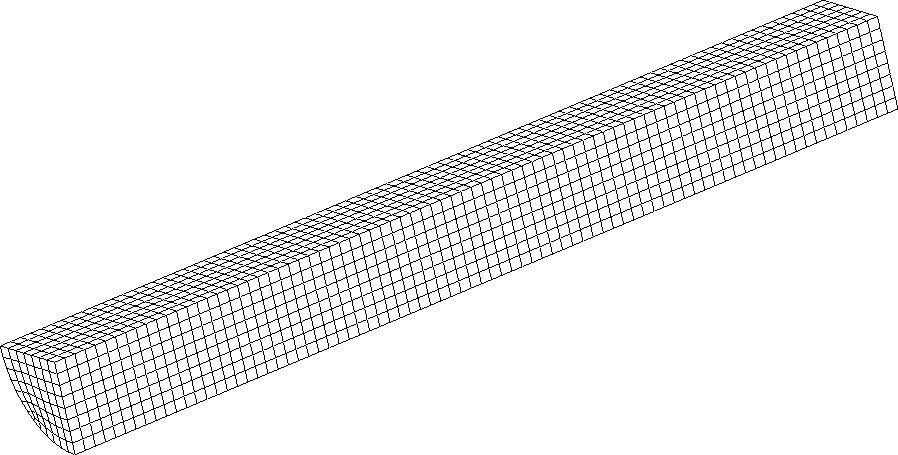
\includegraphics[width=0.5\columnwidth]{Figures/ProgrammingLanguage/mesh}
\par\end{centering}
\caption{Export of a mesh in SVG format\label{fig:PL!SVG!Mesh}}
\end{figure}

\begin{figure}[h]
\begin{centering}
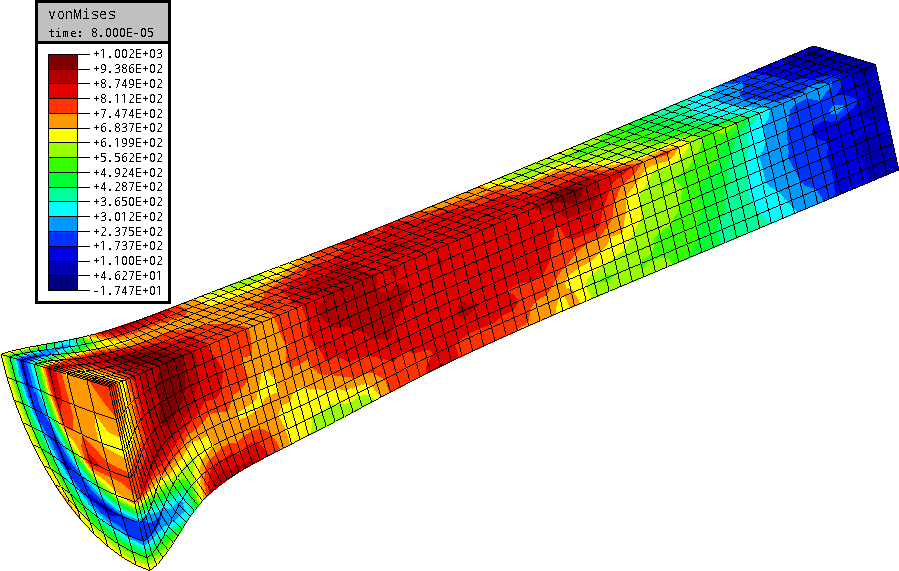
\includegraphics[width=0.5\columnwidth]{Figures/ProgrammingLanguage/vonMisesCP}
\par\end{centering}
\caption{Export of a von Mises contourplot in SVG format\label{fig:PL!SVG!Contourplot}}
\end{figure}

As an illustration, the following commented piece of code has been used to produce both plots presented in Figures \ref{fig:PL!SVG!Mesh} and \ref{fig:PL!SVG!Contourplot}.
\begin{PythonListing}
svg = dnl.SvgInterface('SVG')       # Creates an instance of SvgInterface object
svg.setLegendPosition(100, 280)     # Position the legend
svg.rotate(dnl.Vec3D(0, 1, 0), 190) # Rotation 190 degree around Y axis
svg.rotate(dnl.Vec3D(1, 0, 0), -70) # Rotation -70 degree around X axis
svg.rotate('Y', -60)                # Rotation -60 degree around Y axis
svg.write('mesh.svg')               # Exports the mesh
svg.write('vonMises.svg', dnl.Field.vonMises) # Exports the contourplot
\end{PythonListing}

More details concerning the syntax of the SvgInterface class are presented in the following subsections.

\subsection{Initialization of an SVG object}
Creation of a SVG file under \DynELA is done using through the instantiation of an object \textsf{SvgInterface} object using the following syntax:
\begin{PythonListing}
svg = dnl.SvgInterface('SVG object')
\end{PythonListing}
In this piece of code, \textsf{svg} is an instance of the object \textsf{SvgInterface} and '\emph{SVG object}' is the associated name of the object created by the constructor of the \textsf{SvgInterface} class.

Concerning \textsf{SvgInterface}, \DynELA creates a window with the prescribed size $1600\times1600$, where the coordinates of the top-left corner are $(0, 0)$ and the coordinates of the bottom-right corner are $(1600, 1600)$. All drawing options where some coordinates are requested must conform to this definition.

\subsection{Drawing options}

\subsubsection{View orientation and rotations}
\begin{description}
\item [{resetView ( )}] : This resets the current view to the original one where $O,\overrightarrow{x},\overrightarrow{y}$ is the drawing plane and $\overrightarrow{z}$ is pointing forward.\index[PL]{SvgInterface!resetView( )}
\item [{rotate (\emph{string}, \emph{float})}] : Defines the rotation of the global structure around one of the $3$ base axis referred by the \emph{string} value 'X', 'Y' or 'Z' with an angle $\alpha$ defined by a \emph{float} value.\index[PL]{SvgInterface!rotate(string, float)}
\item [{rotate (\emph{Vec3D}, \emph{float})}] : Defines the rotation of the global structure around the axis $\overrightarrow{v}$ defined by a \emph{Vec3D} with an angle $\alpha$ defined by a \emph{float} value.\index[PL]{SvgInterface!rotate(Vec3D, float)}
\end{description}

\subsubsection{Mesh and data output}
\begin{description}
\item [{setMeshDisplay (\emph{bool} = [true])}] : Set or unset the drawing of the mesh.\index[PL]{SvgInterface!setMeshDisplay(bool)}
\item [{setMeshThickness (\emph{float} = [1.0])}] : Defines the line thickness for drawing the mesh.\index[PL]{SvgInterface!setMeshThickness(float)}
\item [{setPatchLevel (\emph{int} = [1])}] : Defines the level of decomposition of the elements for drawing, \ie the number of recursive decomposition of the polygons [1 to 4]. The default value is usually sufficient for all plots, increasing it enhances the precision of the plot, but drastically increases also the size of the produced file.\index[PL]{SvgInterface!setPatchLevel(int)}
\item [{setAutoRangeValues (\emph{bool} = [true])}] : Set or unset the automatic computation of minimum and maximum values for fields range. This function must be switched to \emph{false} in addition to the function \textsf{setBounds} of the \textsf{colorMap} class (see \ref{sec:PL!SVG!ColorMap}).\index[PL]{SvgInterface!setAutoRangeValues(bool)}
\end{description}

\subsubsection{Legends and notations}
\begin{description}
\item [{setInfoDisplay (\emph{bool} = [false])}] : Set or unset the drawing of the bloc of informations.\index[PL]{SvgInterface!setInfoDisplay(bool)}
\item [{setInfoPosition (\emph{int}, \emph{int})}] : Defines the position of the bloc of informations on the current drawing (default position is $(50, 1200)$).\index[PL]{SvgInterface!setInfoPosition(int, int)}
\item [{setLegendDisplay (\emph{bool} = [true])}] :  Set or unset the drawing of the legend.\index[PL]{SvgInterface!setLegendDisplay(bool)}
\item [{setLegendPosition (\emph{int}, \emph{int})}] : Defines the position of the legend on the current drawing (default position is $(30, 30)$).\index[PL]{SvgInterface!setLegendPosition(int, int)}
\item [{setTitleDisplay (\emph{bool} = [true])}] :  Set or unset the drawing of the title.\index[PL]{SvgInterface!setTitleDisplay(bool)}
\item [{setTitlePosition (\emph{int}, \emph{int})}] : Defines the position of the title on the current drawing (default position is $(50, 1550)$).\index[PL]{SvgInterface!setTitlePosition(int, int)}
\end{description}

\subsubsection{Color Map Options}\label{sec:PL!SVG!ColorMap}
Color Map used for SVG plots can be changed to one of the predefined color-maps using the following syntax (ex: changing for a gray map):
\begin{PythonListing}
svg.colorMap.setGrayMap() # set the color map to Gay
\end{PythonListing}
The following 6 maps are available in \DynELA.
\begin{description}
\item [{setColorMap ( )}] : defines a classic color map.\\
 \hspace*{0.2\columnwidth}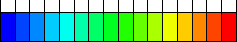
\includegraphics{Figures/ProgrammingLanguage/ColorMap}
\item [{setDeepColorMap ( )}] : defines a deep-color map (this is the \textsf{default} map).\\
 \hspace*{0.2\columnwidth}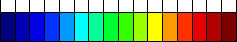
\includegraphics{Figures/ProgrammingLanguage/DeepColorMap}
\item [{setGrayMap ( )}] : defines a gray map.\\
 \hspace*{0.2\columnwidth}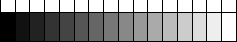
\includegraphics{Figures/ProgrammingLanguage/GrayMap}
\item [{setReverseColorMap ( )}] : defines a reversed classic color map (from red to blue).\\
 \hspace*{0.2\columnwidth}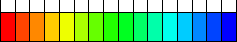
\includegraphics{Figures/ProgrammingLanguage/ReverseColorMap}
\item [{setReverseDeepColorMap ( )}] : defines a reversed deep-color map (from red to blue).\\
 \hspace*{0.2\columnwidth}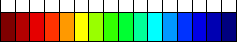
\includegraphics{Figures/ProgrammingLanguage/ReverseDeepColorMap}
\item [{setReverseGrayMap ( )}] : defines a reversed gray map (from white to black).\\
 \hspace*{0.2\columnwidth}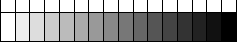
\includegraphics{Figures/ProgrammingLanguage/ReverseGrayMap}
\end{description}

In \DynELA, maps are defined by a given range and number of isovalues. Those parameters can be defined using the following methods:
\begin{description}
\item [{setLevels (\emph{int} = [16]})] : maps are decomposed into the given number of colors, \ie isovalues levels.
\item [{setBounds (\emph{float}, \emph{float})}] : maps are automatically ranged to fit the current field range. But this method allows to fix this range\footnote{In order to use this method it is mandatory to use the method \textsf{setAutoRangeValues} of the \textsf{SvgInterface} class and set it to \emph{false}.}. Out of bounds zones will be drawn in black for low values and white for high values.
\end{description}

On the other hand, the following methods returns some informations on the current map:
\begin{description}
\item [{max ( )}] : get the maximum value of the range.
\item [{min ( )}] : get the minimum value of the range.
\item [{levels ( )}] : get the current number of levels.
\end{description}

\subsection{Creation of the SVG file}
Effective creation of the SVG file is done by calling the \textsf{write} method of the \textsf{SvgInterface} class with the following syntax:\index[PL]{SvgInterface!write(string)}\index[PL]{SvgInterface!write(string, Field)}
\begin{PythonListing}
svg.write('mesh.svg') # Without field, this draws only the mesh
svg.write('temp.svg', dnl.Field.temperature)
\end{PythonListing}
Here, on line number 1, '\emph{temp.svg}' is the name of the SVG file to create for exporting the mesh. On line number 2, '\emph{temp.svg}' is the name of the SVG file to create and \textsf{dnl.Field.temperature} is the name of the associated field to output (see \ref{ProgrammingLanguage:Section:Fields} for definitions).


% !TeX spellcheck = en_US
% !TeX root = DynELA.tex
%
% LaTeX source file of DynELA FEM Code
%
% (c) by Olivier Pantalé 2020
%
\chapter{Curves utility}\label{chap:CU!CU}

\startcontents[chapters]
\printmyminitoc[2]

\LETTRINE{T}his chapter deals about the curves utility of the \DynELA. This curve utility is a Python library used to produce plots (vector or bitmap plots) from \DynELA history files by reading a configuration file describing the way to produce those plots from a simple syntax language. The core of the library uses the matplotlib library implemented using the Python3 language. With this curve utility library, it is therefore possible to produce output graphics and curves directly from the python model file at the end of the solve.

\section{Introduction and presentation of the script}

\subsection{Usage of the Python script}

The Curve library is called from a Python script with the following minimal form.

\begin{PythonListing}
import dnlCurves              # Import the dnlCurve library
curves = dnlCurves.Curves()   # Creates an instance of the Curve object
curves.plotFile('Curves.ex')  # Plot the curves defined by the 'Curves.ex' file
\end{PythonListing}

\subsection{Datafile format}

The datafile format is the plot file used by \DynELA. This file is a text file with $\overrightarrow{x}$ and $\overrightarrow{y}$ datas defined by two or more series of floating point data on two or more columns separated by spaces. This file should contain two header lines on top and should conform to the following for a datafile containing one data.

\begin{PythonListing}
#DynELA_plot history file
#plotted :timeStep
1.0596474E-06 1.0596474E-06
1.0058495E-04 1.0572496E-06
<@\ldots\ldots@>
1.0000000E-02 1.4838518E-07
\end{PythonListing}

In this file, the very first line is ignored by the script, while the second one is used to define the default name of the variable to be plotted (here 'timeStep' in this case). Here after is a example of a datafile containing more columns.

\begin{PythonListing}
#DynELA_plot history file
#plotted :s11 s22 s33
1.0596474E-06 1.0596474E+06 2.0596474E+06 -1.0596474E+06
1.0058495E-04 1.0572496E+06 2.0572496E+06 -1.0572496E+06
<@\ldots\ldots@>
1.0000000E-02 1.4838518E+07 2.4838518E+07 -1.4838518E+07
\end{PythonListing}

In this case, one can specify which columns will be used for plotting the curves as it will be presented just later.

\section{Configuration file to define the plots}

A configuration file is used to define the plots and is read by the \textsf{curves.plotFile()} method of the Curves object. Global parameters are defined using the keyword \textsf{Parameters} at the beginning of a line of the parameter file. The keyword parameter is followed by a set of commands used to set some global parameters for all the subsequent generated graphs by overwriting the default parameters, before generating the very first graph.

\begin{PythonListing}
Parameters, xname=Displacement x, crop=True
\end{PythonListing}

Then all parameters can also be altered within the definition of a plot. A definition of a plot is done by a line without the \textsf{Parameters} keyword. The first element on this line is the name of the generated graph, followed by a set of parameters defining the generated plot.

\begin{PythonListing}
# Plot of Temp.plot to Temp.svg file
Temp, name=$T$, Temp.plot
# Plot of column 1 of Stress.plot file to S11.svg file
S11, name=$\sigma_{xx}$, legendlocate=topleft, Stress.plot[0:1]
# Plot of column 2 of Stress.plot file to S22.svg file
S22, name=$\sigma_{yy}$, legendlocate=bottomleft, Stress.plot[0:2]
# Plot of dt.plot and Abaqus/Step.plot files to TimeStep.svg file
TimeStep, name=$\Delta t$, dt.plot, name=$Abaqus \Delta t$, Abaqus/Step.plot
\end{PythonListing}

In the proposed example we have the following.
\begin{itemize}
\item Line 2: plots the content of the Temp.plot file with legend $T$ in a Temp.svg file using default parameters.
\item Line 4: plots the content of the Stress.plot file with legend $\sigma_{xx}$ in a S11.svg file using data from columns $0$ for $\overrightarrow{x}$ and from column $1$ for $\overrightarrow{y}$ and with a legend located in the top left part of the figure.
\item Line 6: plots the content of the Stress.plot file with legend $\sigma_{yy}$ in a S22.svg file using data from columns $0$ for $\overrightarrow{x}$ and from column $2$ for $\overrightarrow{y}$ with a legend located in the bottom left part of the figure.
\item Line 8: plots the content of the dt.plot file with legend $\Delta t$ and Abaqus/Step.plot file with legend $Abaqus\,\Delta t$ in a TimeStep.svg file.
\end{itemize}

As presented just before, \LaTeX~can be used for names and legends by using the escape character $\$$ and remembering that space character has to be defined by the combination of an escape '\textbackslash' character followed by the space '~' so that '\textbackslash~'.

Comments can be inserted as presented briefly earlier by using the '\#' character. Everything after the '\#' character and up to the end of the line is ignored and treated as comment. Blank lines are also allowed in the file to help human readability of the file.

\subsection{Global parameters for a graph}
\begin{description}
\item [outputformat = <'format'>]: is used to define the format of the output file, \ie pdf, svg, png,\ldots (default value is svg file).
\item [transparent = <True, False>]: is used to define if the background should be or not transparent (default value is False).
\item [crop = <True, False>]: is used to define if the output image should be or not cropped (default value is False).
\item [grid = <True, False>]: is used to define if the output graph should contain or not a grid (default value is True).
\item [title = <'name'>]: defines the title of the graph on the top part of the plot ( default value 'Default title of the graph')
\item [xname, yname = <'name'>]: defines the names of the $\overrightarrow{x}$ and $\overrightarrow{y}$ axis for the plot (default value are 'x-axis' and 'y-axis').
\item [titlefontsize = <size>]: defines the font size of the title on the top part of the plot (default value is $20$).
\item [xfontsize, yfontsize = <size>]: defines the font size of the $\overrightarrow{x}$ and $\overrightarrow{y}$ axis names for the plot (default value is $20$).
\item [xlabelfontsize, ylabelfontsize = <size>]: defines the font size of the values along the $\overrightarrow{x}$ and $\overrightarrow{y}$ axis for the plot (default value is $16$).
\item [xrange, yrange = <range>]: remaps the range of the curves for the $\overrightarrow{x}$ and $\overrightarrow{y}$ axis to the given value. For example, setting \textsf{xrange=10} will remap the x-data within the range $[0,10]$.
\item [xscale, yscale = <range>]: multiply the $\overrightarrow{x}$ or the $\overrightarrow{y}$ data by a given factor. For example, setting \textsf{xscale=10} will multiply all x-data by a factor of $10$.
\end{description}

\subsection{Plotting curve parameters}
\begin{description}
\item [name = <'name'>]: defines a new name for the next curve in the legend and overrides the one defined by the datafile.
\item [removename = <'name'>]: removes from the names of the curves a given pattern for the legends. Example: \textsf{removename} = -S11 will convert 'data-S11' into 'data'. This is not a very useful method and one should prefer the \textsf{name} command to redefine the name of the plotting curve.
\item [linewidth = <'width'>]: defines the line width for all subsequent plots (default value is $2$).
\item [marks = <'symbol'>]: is used to define the next marker to use for all subsequent plots (default value is ''). If the value is void, markers are cycled through the default markers list.
\item [marksnumber = <number>]: defines the total number of markers on the curves for all subsequent plots (default value is $20$).
\item [markersize = <size>]: defines the size of the marker symbols to use for all subsequent plots (default value is $10$).
\end{description}

\subsection{Legend definition}
\begin{description}
\item [legendcolumns = <columns>]: defines the number of columns to use for the legend (default value is $1$).
\item [legendshadow = <True, False>]: is used to define if the output graph legend should contain or not a shadow box (default value is True).
\item [legendanchor = <'position'>]: defines the position of the legend anchor independently from the legend position parameter.
\item [legendposition = <'position'>]: defines the position of the legend position independently from the legend anchor parameter.
\item [legendlocate = <'position'>]: defines the position of the legend with the following four options: 'topleft', 'topright', 'bottomleft' and 'bottomright' (default value is 'topright').
\item [legendfontsize = <size>]: defines the font size of the text in the legend (default value is $16$).
\end{description}



% !TeX spellcheck = en_US
% !TeX root = DynELA.tex
%
% LaTeX source file of DynELA FEM Code
%
% (c) by Olivier Pantalé 2020
%
\chapter{Abaqus extractor utility}

\startcontents[chapters]
\printmyminitoc[1]
\LETTRINE{T}his chapter deals about the Abaqus extractor utility of the \DynELA. This extractor is a Python library used to extract results from an Abaqus \textsf{odb} datafile by reading a configuration file describing the way to produce those extracts from a simple syntax language.

\section{Introduction and presentation of the script}

The \textsf{AbaqusExtract} library is called from a Python script with the following minimal form.

\begin{PythonListing}
# import the AbaqusExtract library
import AbaqusExtract
# Extract data using datafile Extract.ex
AbaqusExtract.AbaqusExtract('Extract.ex')
\end{PythonListing}

Assuming that the Python script containing this piece of code is named \textsf{'Extract.py'}, therefore this script must be called from the Abaqus main program using the following command:

\begin{BashListing}
abaqus python Extract.py
\end{BashListing}

\section{Syntax of the configuration file}

Different forms are used depending on the nature of the data to extract, but everything conforms to the Abaqus Python command syntax. The \textsf{AbaqusExtract} library uses some keywords to define the nature of the data to extract as proposed here after.
\begin{description}
\item [TimeHistory]: is a keyword defining that the line contains the instructions to extract a time history from an Abaqus \textsf{odb} file.
\item [job]: is used to define the name of the odb file to use for the extraction of the results \ie it's the name of the \textsf{odb} file without the extension \textsf{.odb}.
\item [value]: is the nature of the variable to extract conforming to the variables names of Abaqus.
\item [name]: is the given name of the plotting file to generate, \ie the name of the plotting file without the \textsf{.plot} extension.
\item [region]: is used to define the location of the data to extract. This one is more complex, as it can be a global location, a node location or an integration point location as described hereafter.
\item [operate]: is an optional parameter defining what to do when multiple regions are defined.
\end{description}
As an example, the following piece of code gives some application examples.

\begin{PythonListing}
# Extraction of a time history node data
TimeHistory, job=Torus, value=U1, name=dispX, region=Node PART-1.3
# Extraction of a time history integration point data
TimeHistory, job=Torus, value=MISES, name=vM, region=Element PART-1.25 Int Point 1
# Extraction of a time history global variable
TimeHistory, job=Torus, value=DT, name=timeStep, region=Assembly ASSEMBLY
\end{PythonListing}

In the previous example:
\begin{itemize}
\item line $2$ is used to extract the nodal displacement \textsf{U1} from the odb file \textsf{Torus.odb} and produce the \textsf{dispX.plot} file for node $3$ of the \textsf{PART-1} piece.
\item line $4$ is used to extract the integration point value \textsf{MISES} from the odb file \textsf{Torus.odb} and produce the \textsf{vM.plot} file for integration point $1$ of element $25$ of the \textsf{PART-1} piece.
\item line $6$ is used to extract the global timestep \textsf{DT} from the odb file \textsf{Torus.odb} and produce the \textsf{timeStep.plot} file.
\end{itemize}
Concerning the definition of the region to use, it is possible to define more than $1$ region by using the \textsf{'+'} sign in the definition of the region. When this is used, the optional parameter operate is used to define what to do with this multiple data. The operation is defined by:
\begin{description}
\item [operate = none]: or no operate parameter defined, therefore, all values are reported to the plotting file separated by a white space.
\item [operate = mean]: the mean value is computed and reported to the plotting file.
\item [operate = sum]: the sum of the values is computed and reported= to the plotting file.
\end{description}



\cleardoublepage

\part{DynELA Samples}

% !TeX spellcheck = en_US
% !TeX root = DynELA.tex
%
% LaTeX source file of DynELA FEM Code
%
% (c) by Olivier Pantalé 2020
%
\chapter{DynELA single element sample cases}

\startcontents[chapters]
\printmyminitoc[2]\LETTRINE{T}his chapter deals with some numerical applications of
the \DynELA for dynamic applications in 2D, axi-symmetric and 3D
cases. In the subsequent tests, if not specified, a Johnson-Cook constitutive
law is used to model the behavior of the material. The Johnson-Cook
hardening flow law is probably the most widely used flow law for the
simulation of high strain rate deformation processes taking into account
plastic strain, plastic strain rate and temperature effects. Since
a lot of efforts have been made in the past to identify the constitutive
flow law parameters for many materials, it is implemented in numerous
Finite Element codes such as Abaqus \cite{abaqus20146}. The general
formulation of the Johnson-Cook law $\sigma^{y}(\overline{\varepsilon}^{p},\stackrel{\bullet}{\overline{\varepsilon}^{p}},T)$
is given by the following equation:

\begin{equation}
\sigma^{y}=\left(A+B\overline{\varepsilon}^{p^{n}}\right)\left[1+C\ln\left(\frac{\stackrel{\bullet}{\overline{\varepsilon}^{p}}}{\stackrel{\bullet}{\overline{\varepsilon}_{0}}}\right)\right]\left[1-\left(\frac{T-T_{0}}{T_{m}-T_{0}}\right)^{m}\right]\label{eq:Samples!Johnson-Cook}
\end{equation}
where $\stackrel{\bullet}{\overline{\varepsilon}_{0}}$ is the reference
strain rate, $T_{0}$ and $T_{m}$ are the reference temperature and
the melting temperature of the material respectively and $A$, $B$,
$C$, $n$ and $m$ are the five constitutive flow law parameters.
A 42CrMo4 steel following the Johnson-Cook behavior law has been selected
for all those tests, and material properties are reported in Table
\ref{tab:Samples!JohnsonCookParameters}.

\begin{table}[h]
\begin{center}\begin{tcolorbox}[width=.75\textwidth,myTab,tabularx={C|C|C|C|C|C|C}]
$E$ & $\nu$ & $A$ & $B$ & $C$ & $n$ & $m$ \\
\small{($Gpa$)} &  & \small{($MPa$)} & \small{($MPa$)} &  &  & \\ \hline
$206.9$ & $0.3$ & $806$ & $614$ & $0.0089$ & $0.168$ & $1.1$ \\ \hline\hline
$\rho$ & $\lambda$ & $C_{p}$ & $\eta$ & $\stackrel{\bullet}{\overline{\varepsilon}_{0}}$ & $T_{0}$ & $T_{m}$ \\
\small{$(kg/m^{3})$} & \small{$(W/m^{\circ}C)$} & \small{$(J/Kg^{\circ}C)$} & & \small{$(s^{-1})$} & \small{$(^{\circ}C)$} & \small{$(^{\circ}C)$} \\ \hline
$7830$ & $34.0$ & $460$ & $0.9$ & $1.0$ & $20$ & $1540$
\end{tcolorbox}\end{center}

\caption{Material parameters of the Johnson-Cook behavior for the numerical
tests\label{tab:Samples!JohnsonCookParameters}}
\end{table}


\section{Uniaxial tensile tests}

\subsection{Element plane tensile test}

The uniaxial one element tensile test is a numerical test where an
plane element (with a square prescribed shape) is subjected to pure
tensile as presented in figure \ref{fig:Samples!Single!Tensile}.
\begin{figure}[h]
\begin{centering}
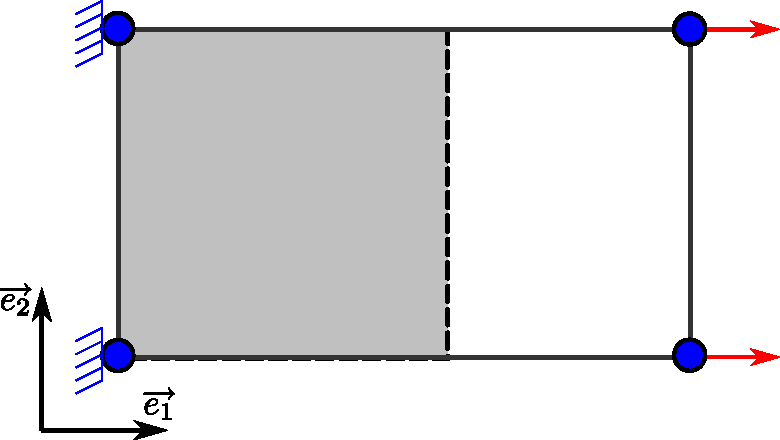
\includegraphics[width=0.5\columnwidth]{Figures/SamplesSingleTensile}
\par\end{centering}
\caption{Numerical model for the one element tensile test\label{fig:Samples!Single!Tensile}}
\end{figure}
 The initial shape of the specimen is $10\,mm\times10\,mm$, the two
left nodes of the element are encastred and a prescribed horizontal
displacement $d=10\,mm$ is applied on the two right nodes of the
same element as illustrated in Figure \ref{fig:Samples!Single!Tensile}.
As we are using an explicit integration scheme, the total simulation
time is set to $t=0.01\,s$.

All the properties of the constitutive law reported in Table \ref{tab:Samples!JohnsonCookParameters}
are used and the material is assumed to follow the Johnson-Cook behavior
described by equation \ref{eq:Samples!Johnson-Cook}.

Figure \ref{fig:Samples!Single!Tensile-Comparison} shows the comparison
of the DynELA solver results (plotted in red) and the Abaqus numerical
results (plotted in blue) concerning the evolution of the stress components
$\sigma_{11}$, $\sigma_{22}$, $\sigma_{12}$, $\overline{\sigma}$,
$\overline{\varepsilon}^{p}$ and $T$ \versus  the horizontal displacement
of the right edge of the specimen along the horizontal axis. For the
Abaqus model, the exact same mesh has been used. Comparison of Abaqus
and DynELA results is made by averaging the DynELA results on the
$4$ integration points of the element. This has been done because
\DynELA uses full integrated elements while Abaqus have reduced
integrated elements only but in fact, the DynELA results at the $4$
integration points are the same in this benchmark test.

\begin{figure}[h]
\begin{centering}
\begin{tabular}{cc}
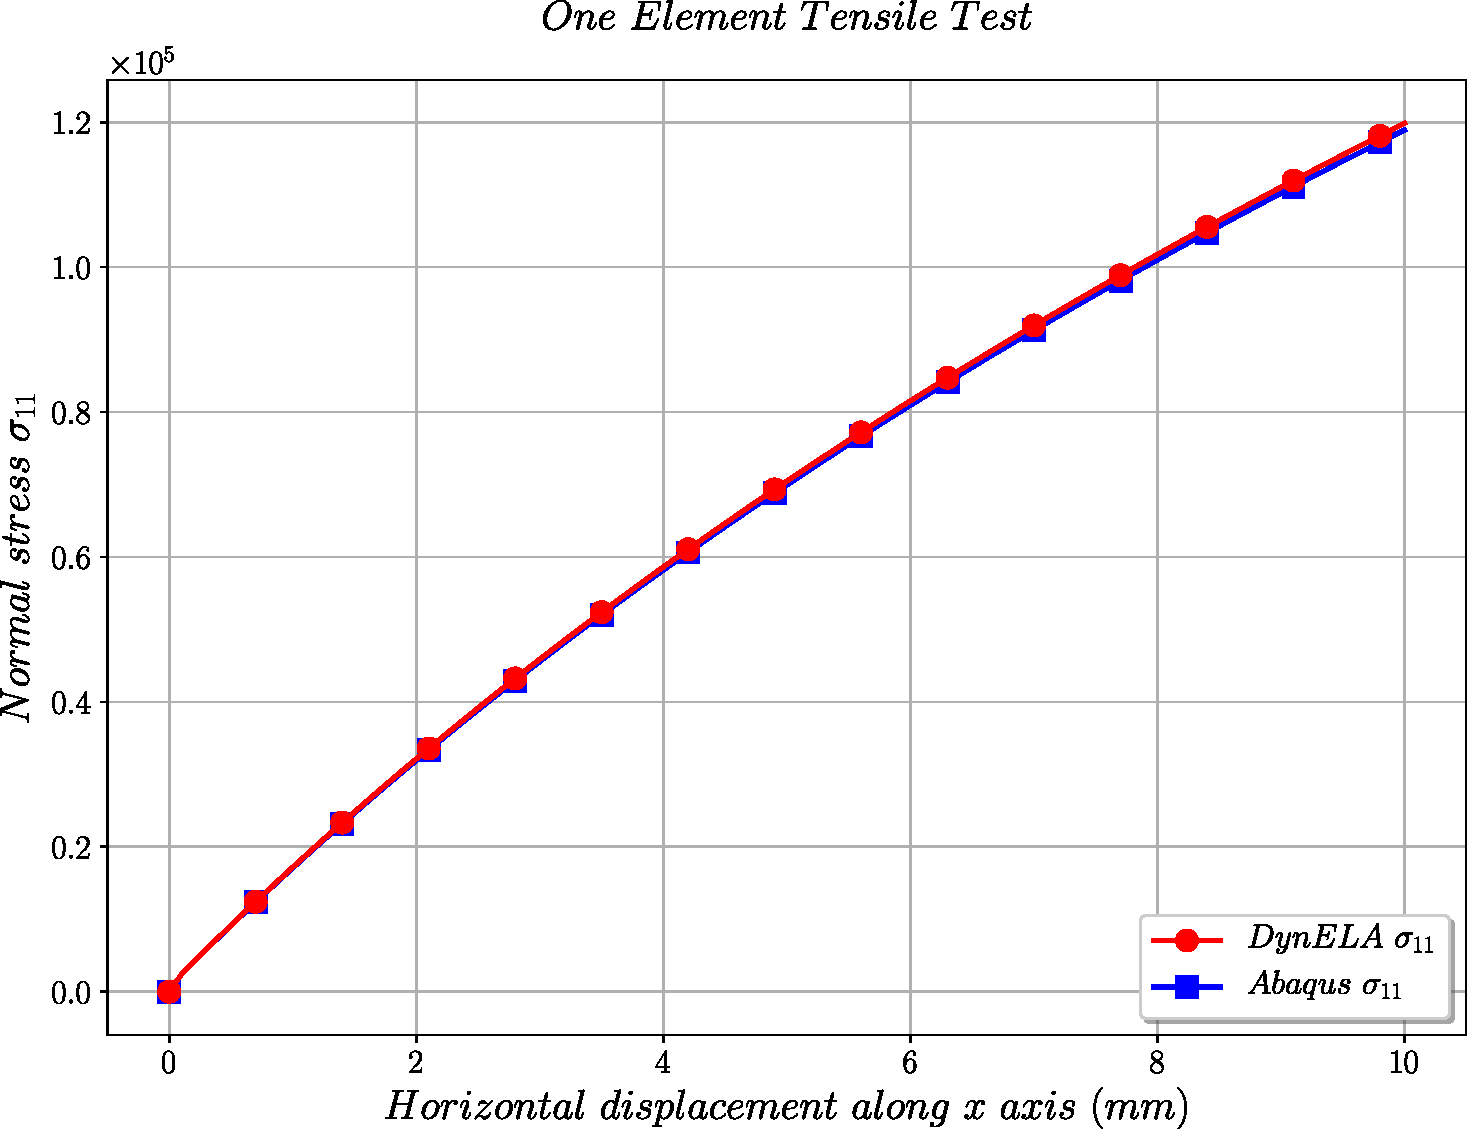
\includegraphics[width=0.45\columnwidth]{Figures/Samples/Element/Tensile_stress_11} & 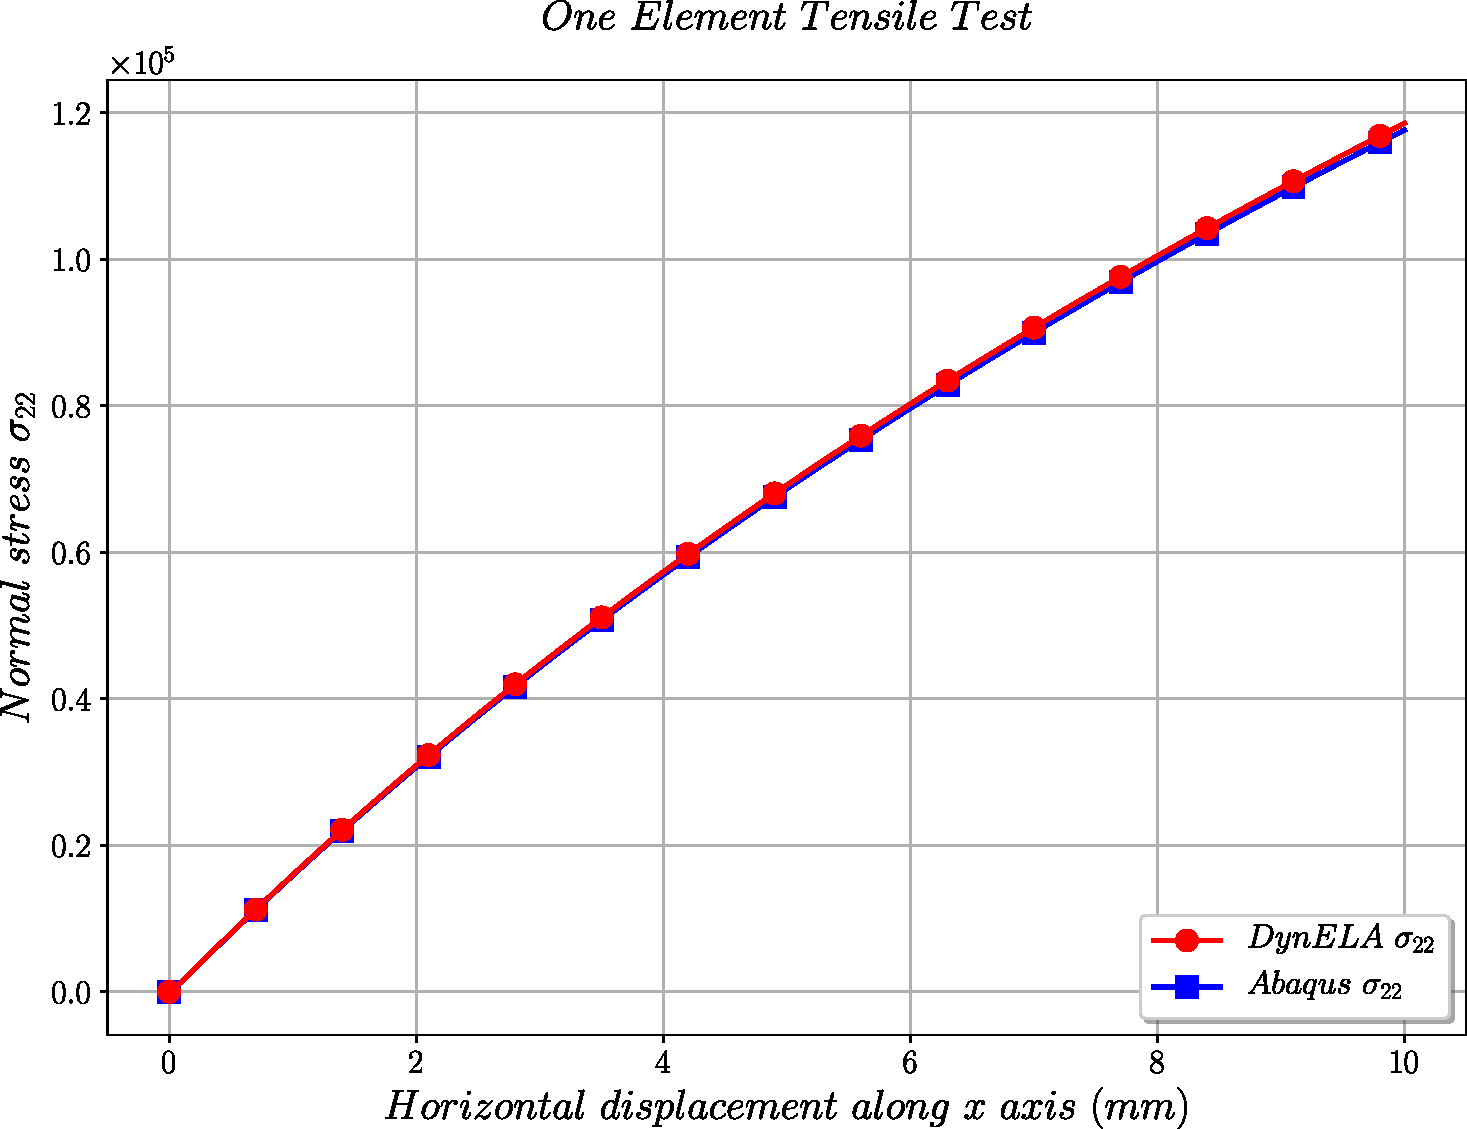
\includegraphics[width=0.45\columnwidth]{Figures/Samples/Element/Tensile_stress_22}\tabularnewline
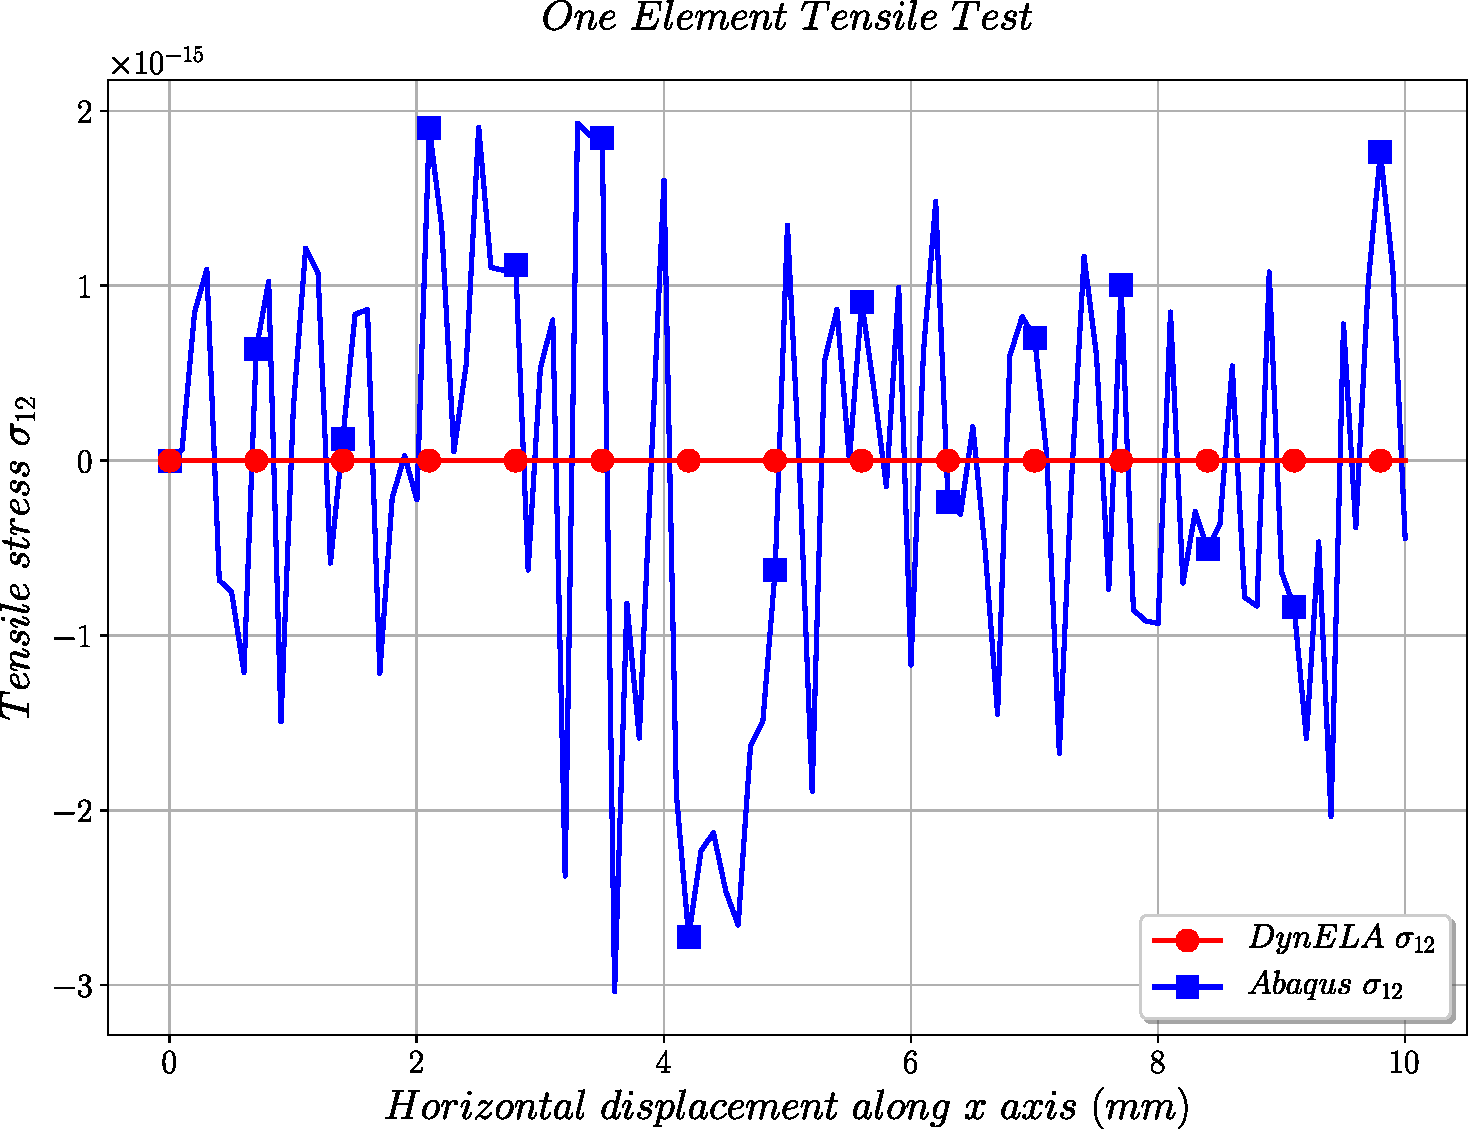
\includegraphics[width=0.45\columnwidth]{Figures/Samples/Element/Tensile_stress_12} & 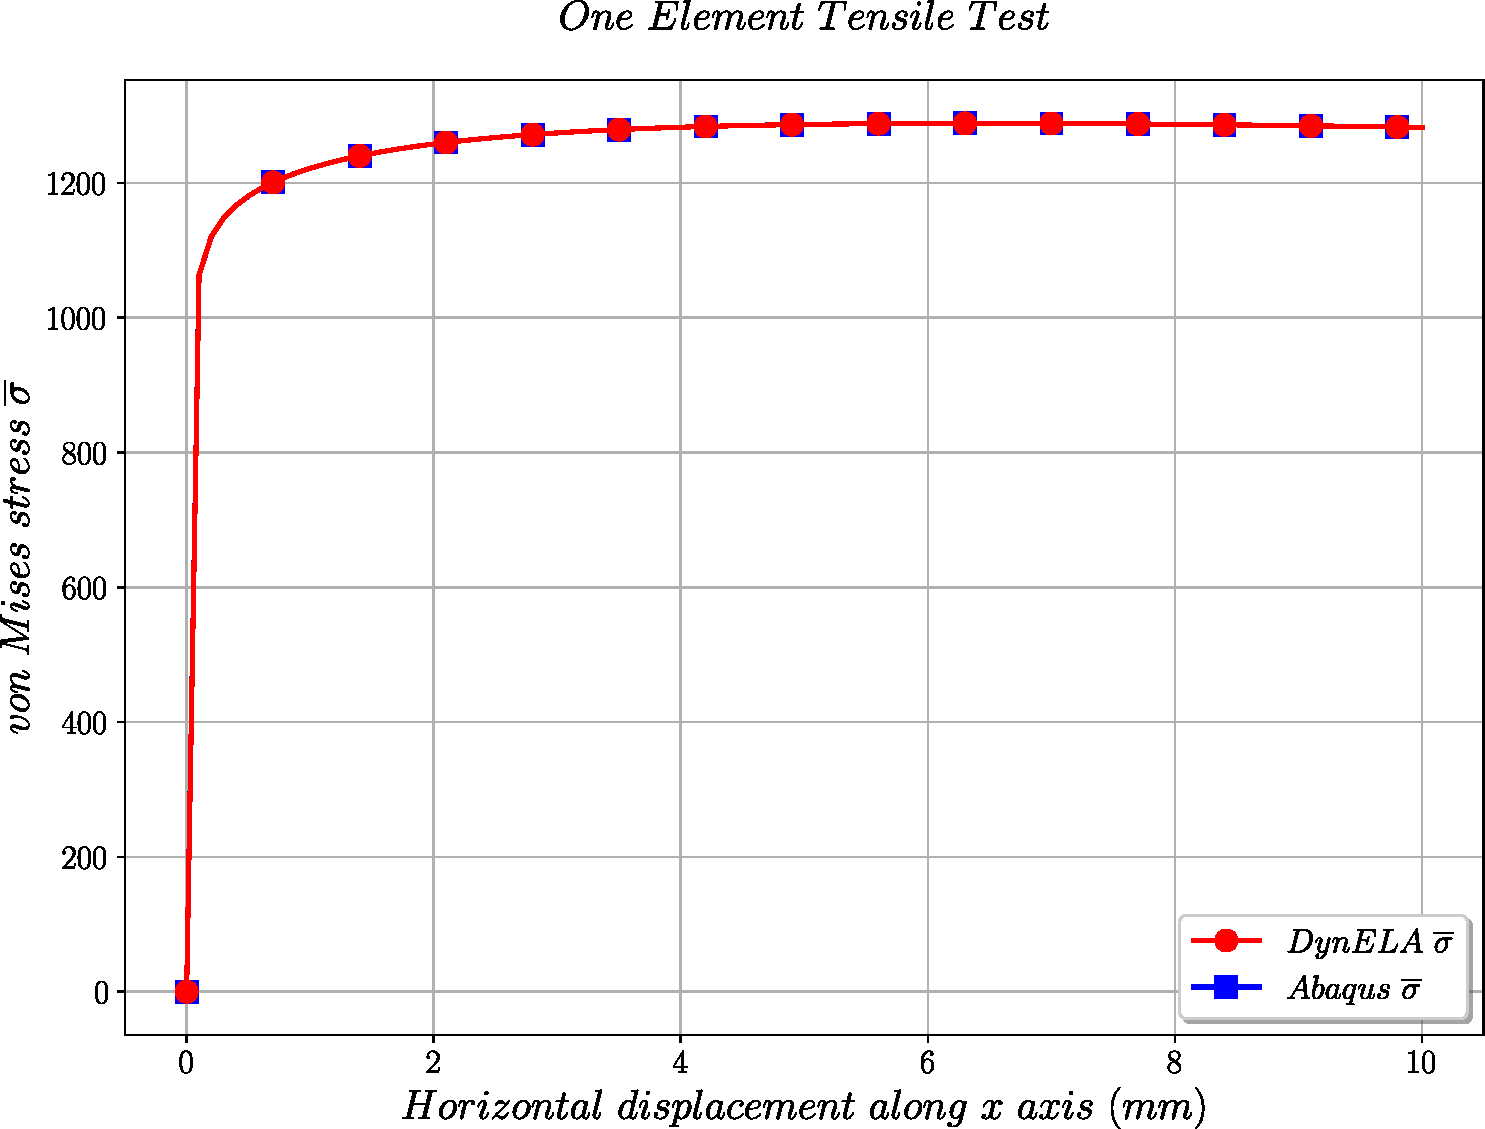
\includegraphics[width=0.45\columnwidth]{Figures/Samples/Element/Tensile_vonMises}\tabularnewline
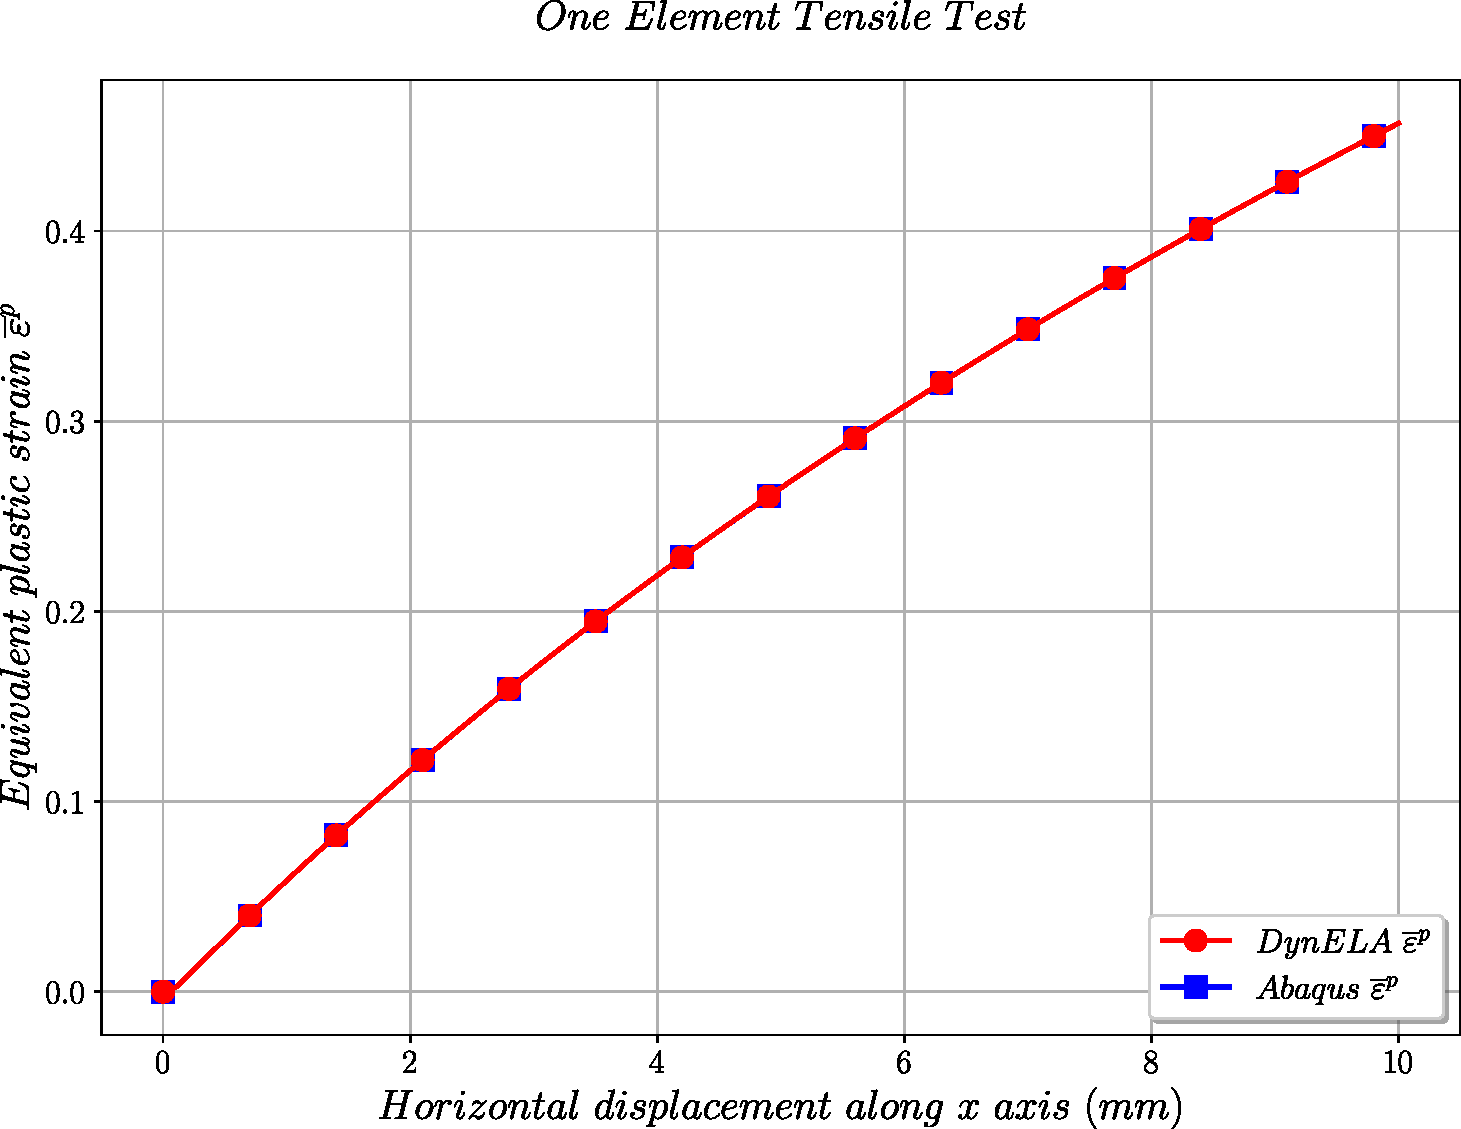
\includegraphics[width=0.45\columnwidth]{Figures/Samples/Element/Tensile_plasticStrain} & 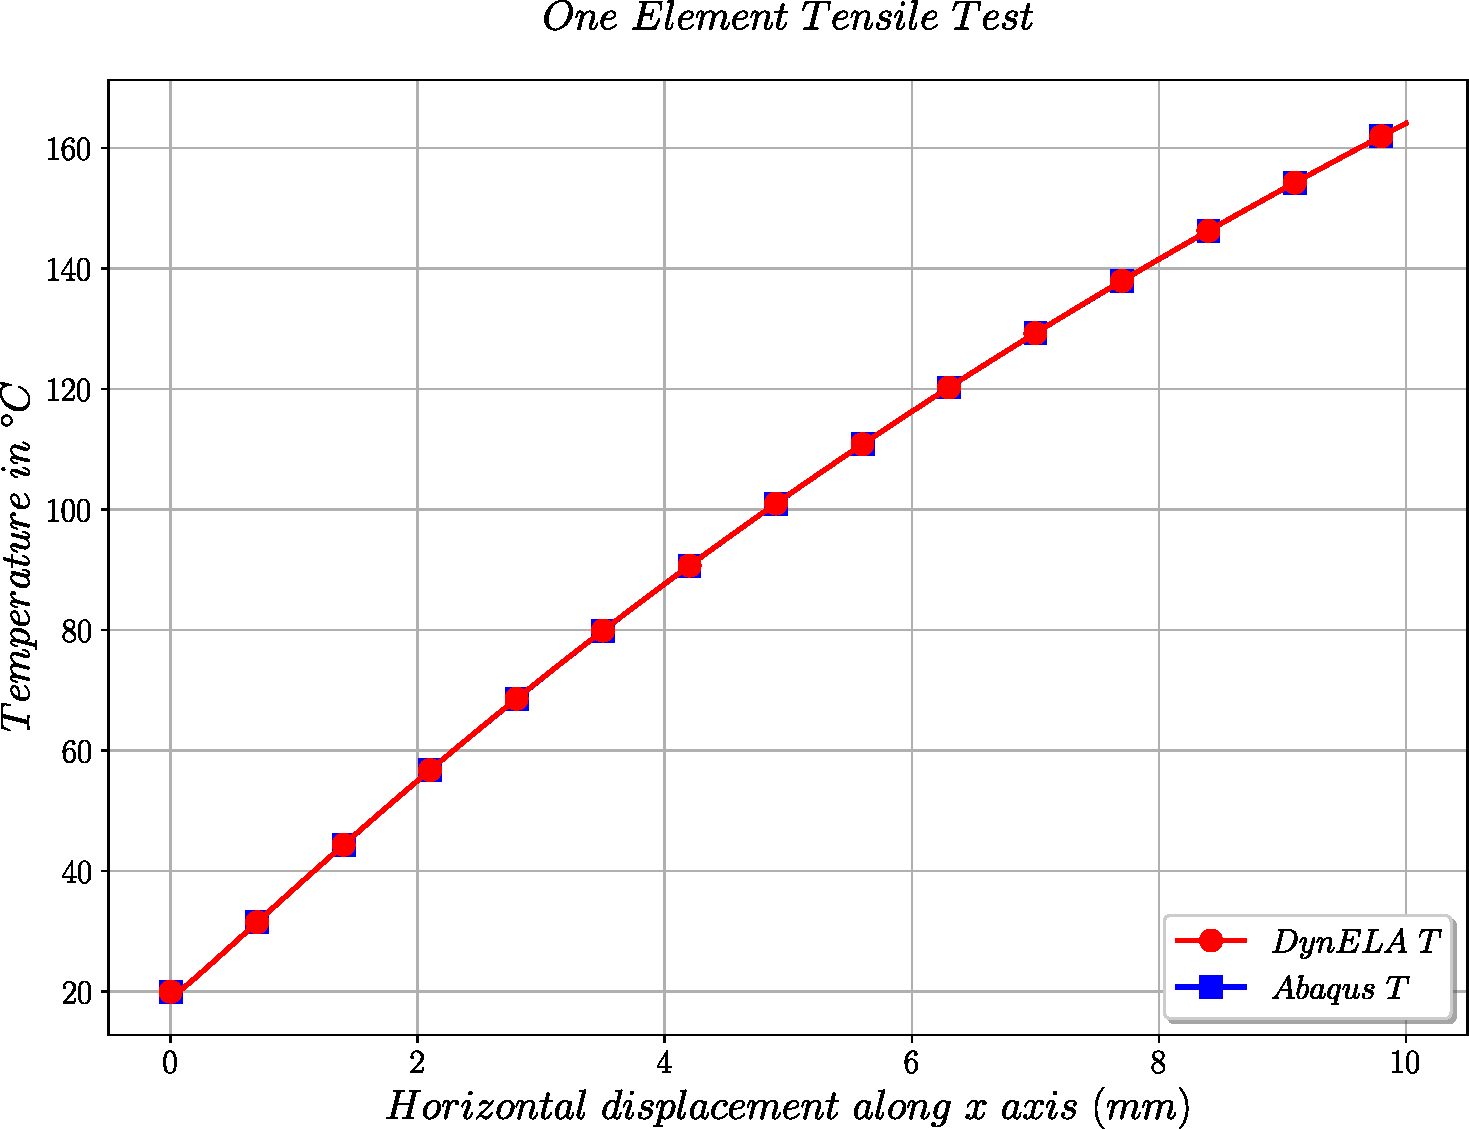
\includegraphics[width=0.45\columnwidth]{Figures/Samples/Element/Tensile_temperature}\tabularnewline
\end{tabular}
\par\end{centering}
\caption{Comparison of numerical and analytical results for the one element
tensile test\label{fig:Samples!Single!Tensile-Comparison}}
\end{figure}
\clearpage

\subsection{Element 3D tensile test}

The uniaxial one element 3D tensile test is a numerical test where
a 3D brick element (with a cubic prescribed shape) is subjected to
radial tensile as presented in figure \ref{fig:Samples!Single!Tensile-3D}.
No boundary condition has been prescribed on the $\overrightarrow{z}$
direction, so that the reduction of the width during the test can
occur. The initial shape of the specimen is $10\,mm\times10\,mm\times10\,mm$
and the the two left nodes of the element are restrained for their
displacements along the $\overrightarrow{x}$ and $\overrightarrow{y}$
directions and a prescribed horizontal displacement $d=10\,mm$ is
applied on the two right nodes of the same element as illustrated
in Figure \ref{fig:Samples!Single!Tensile-3D}. As we are using an
explicit integration scheme, the total simulation time is set to $t=0.01\,s$.
\begin{figure}[h]
\begin{centering}
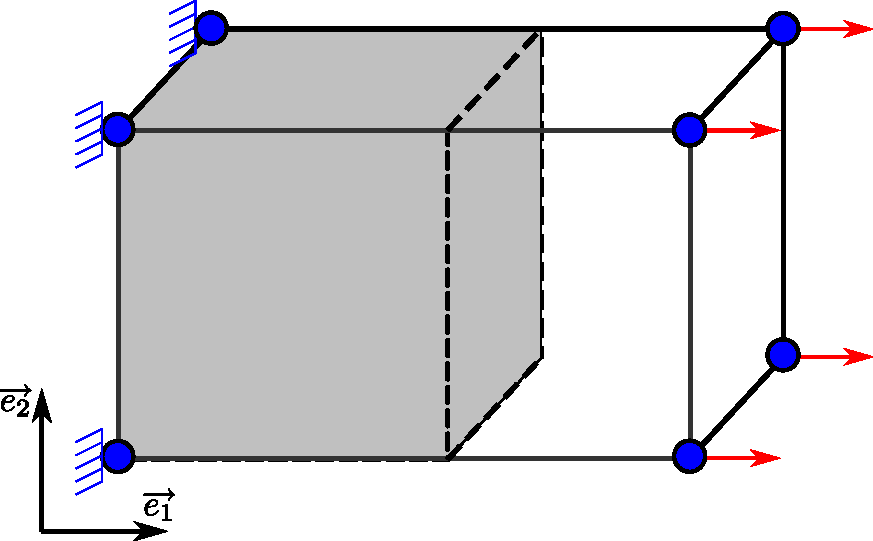
\includegraphics[width=0.5\columnwidth]{Figures/SamplesSingleTensile3D}
\par\end{centering}
\caption{Numerical model for the one element tensile test\label{fig:Samples!Single!Tensile-3D}}
\end{figure}

All the properties of the constitutive law reported in Table \ref{tab:Samples!JohnsonCookParameters}
are used and the material is assumed to follow the Johnson-Cook behavior
described by equation \ref{eq:Samples!Johnson-Cook}.

Figure \ref{fig:Samples!Single!Tensile-Comparison-3D} shows the comparison
of the DynELA solver results (plotted in red) and the Abaqus numerical
results (plotted in blue) concerning the evolution of the stress components
$\sigma_{11}$, $\sigma_{22}$, $\sigma_{12}$, $\overline{\sigma}$,
$\overline{\varepsilon}^{p}$ and $T$ \versus  the horizontal displacement
of the right edge of the specimen along the horizontal axis. For the
Abaqus model, the exact same mesh has been used. Comparison of Abaqus
and DynELA results is made by averaging the DynELA and the Abaqus
results on the $8$ integration points of the element.

\begin{figure}[h]
\begin{centering}
\begin{tabular}{cc}
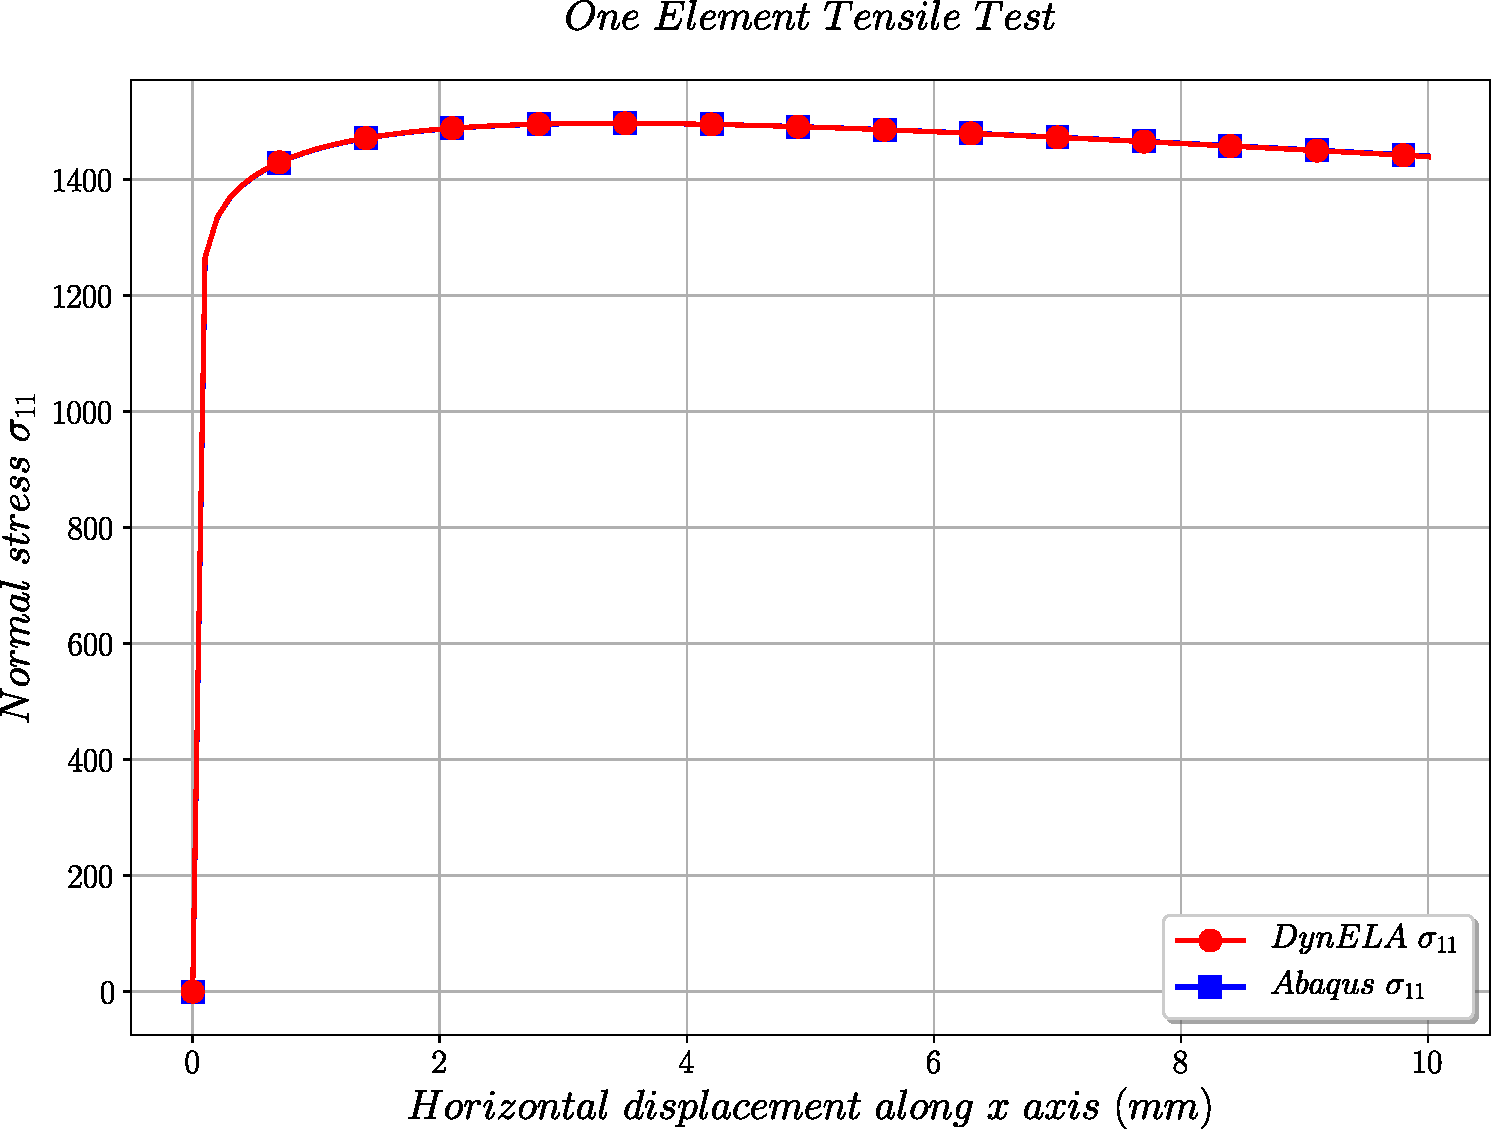
\includegraphics[width=0.45\columnwidth]{Figures/Samples/Element/Tensile3D_stress_11} & 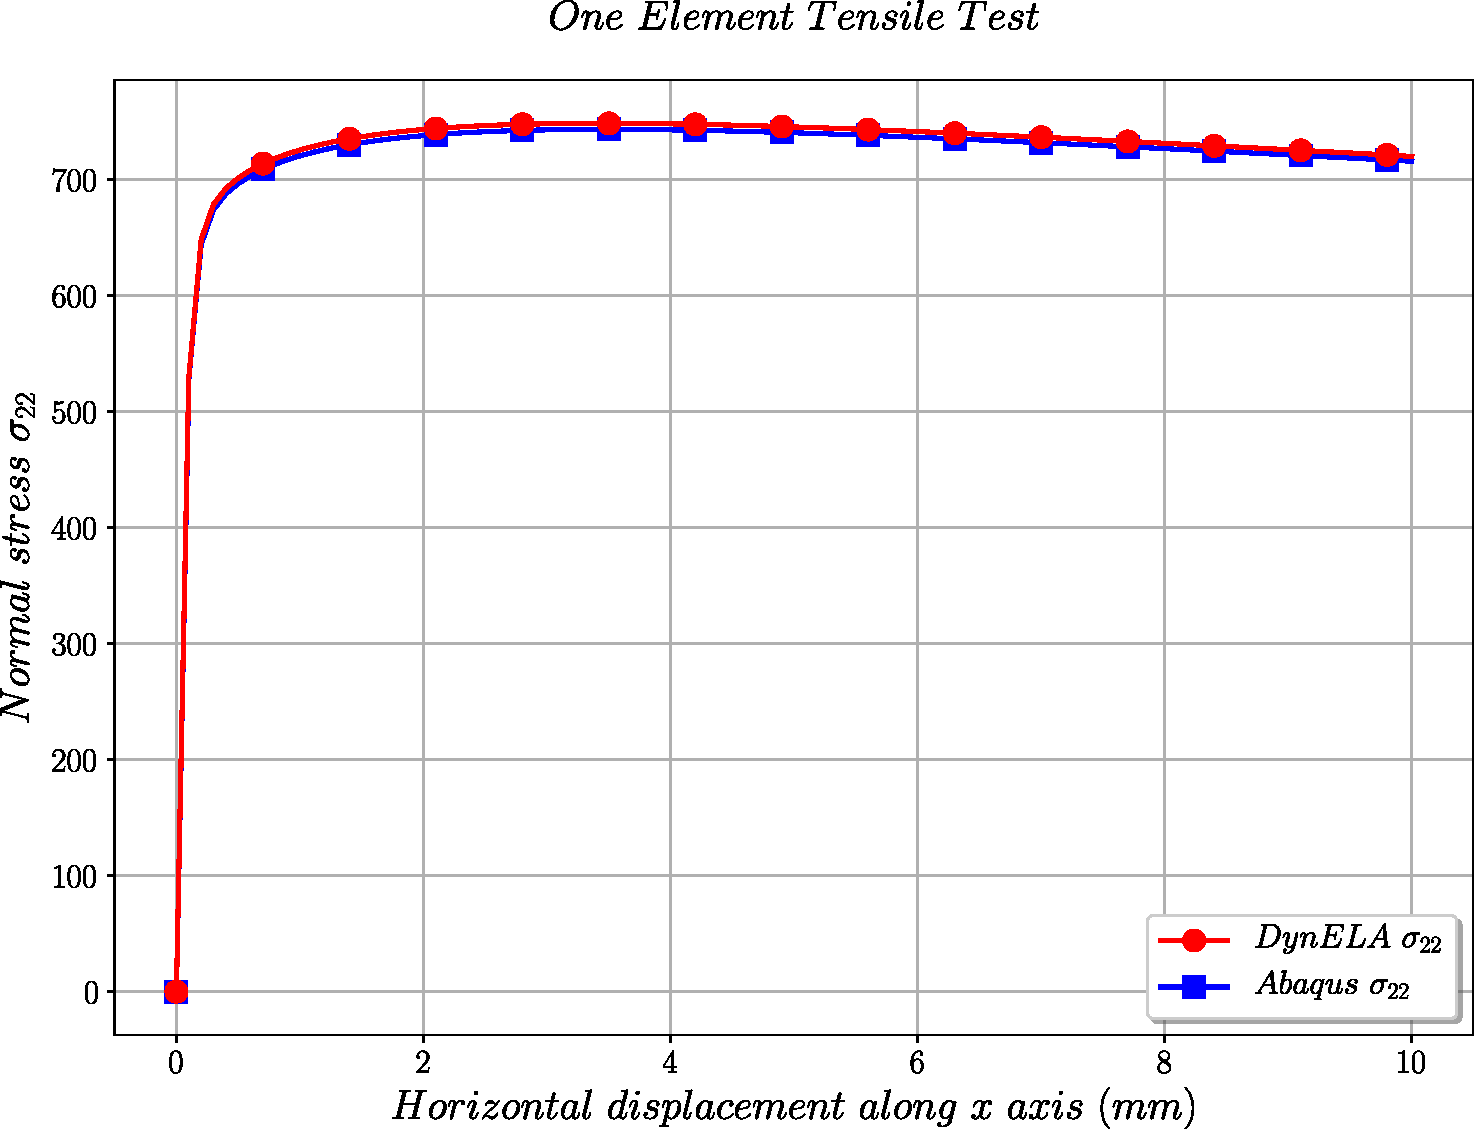
\includegraphics[width=0.45\columnwidth]{Figures/Samples/Element/Tensile3D_stress_22}\tabularnewline
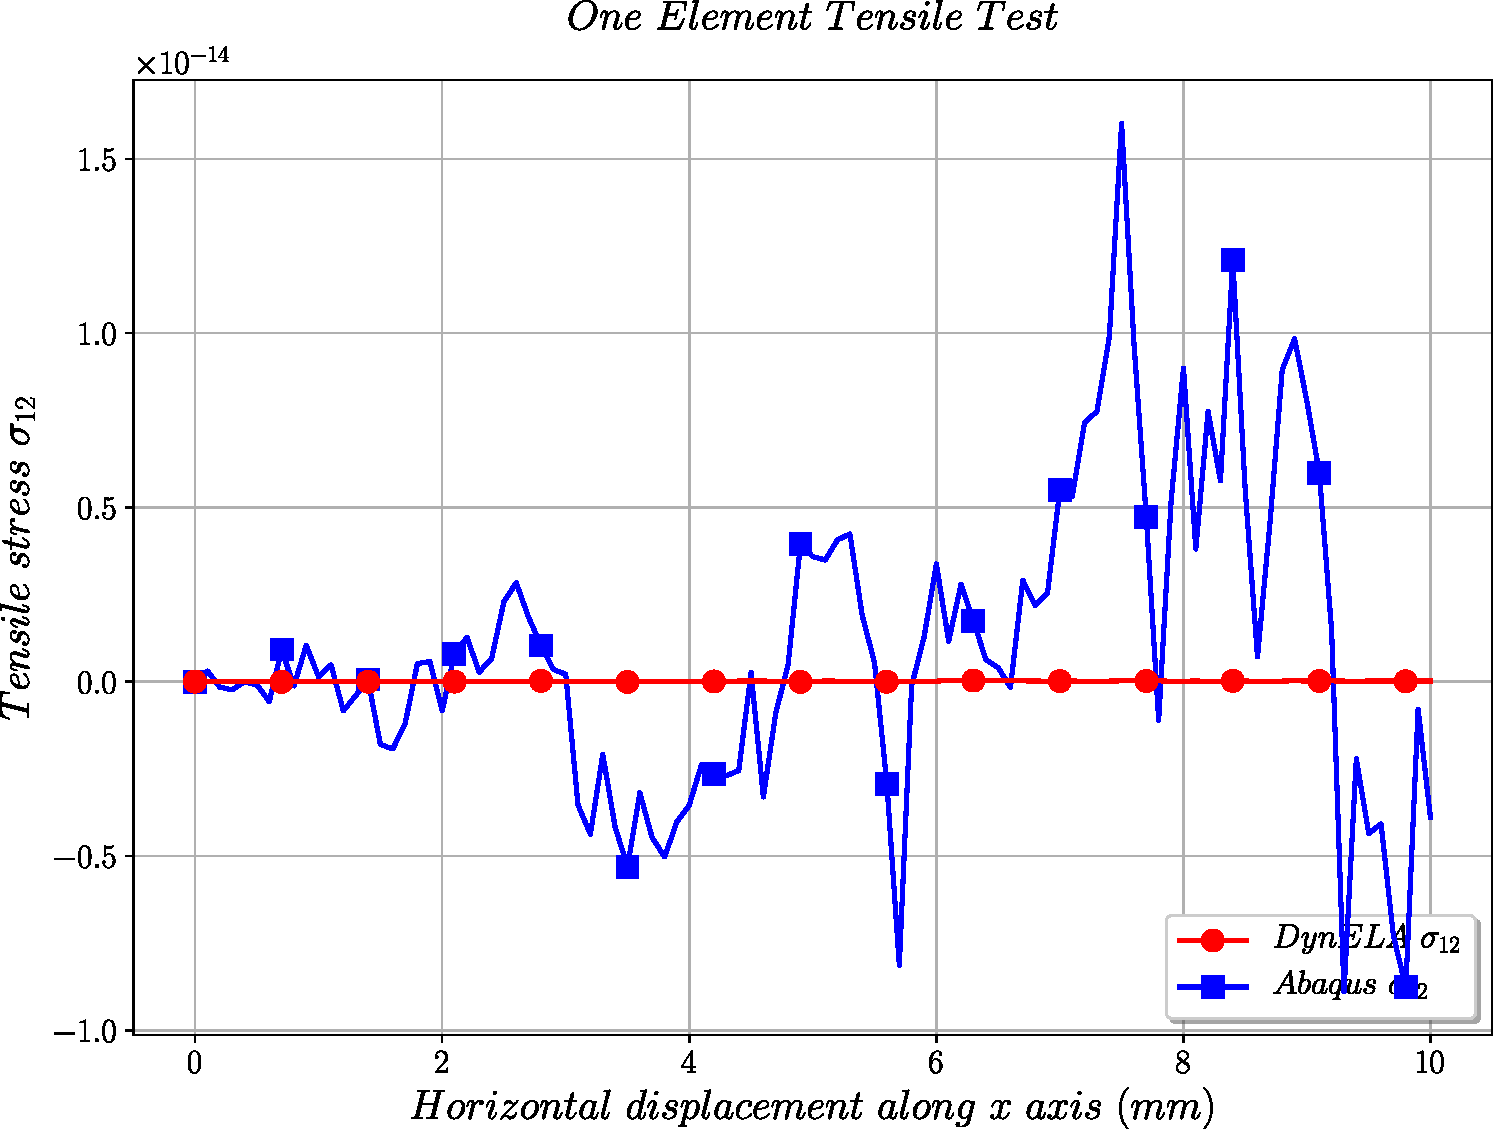
\includegraphics[width=0.45\columnwidth]{Figures/Samples/Element/Tensile3D_stress_12} & 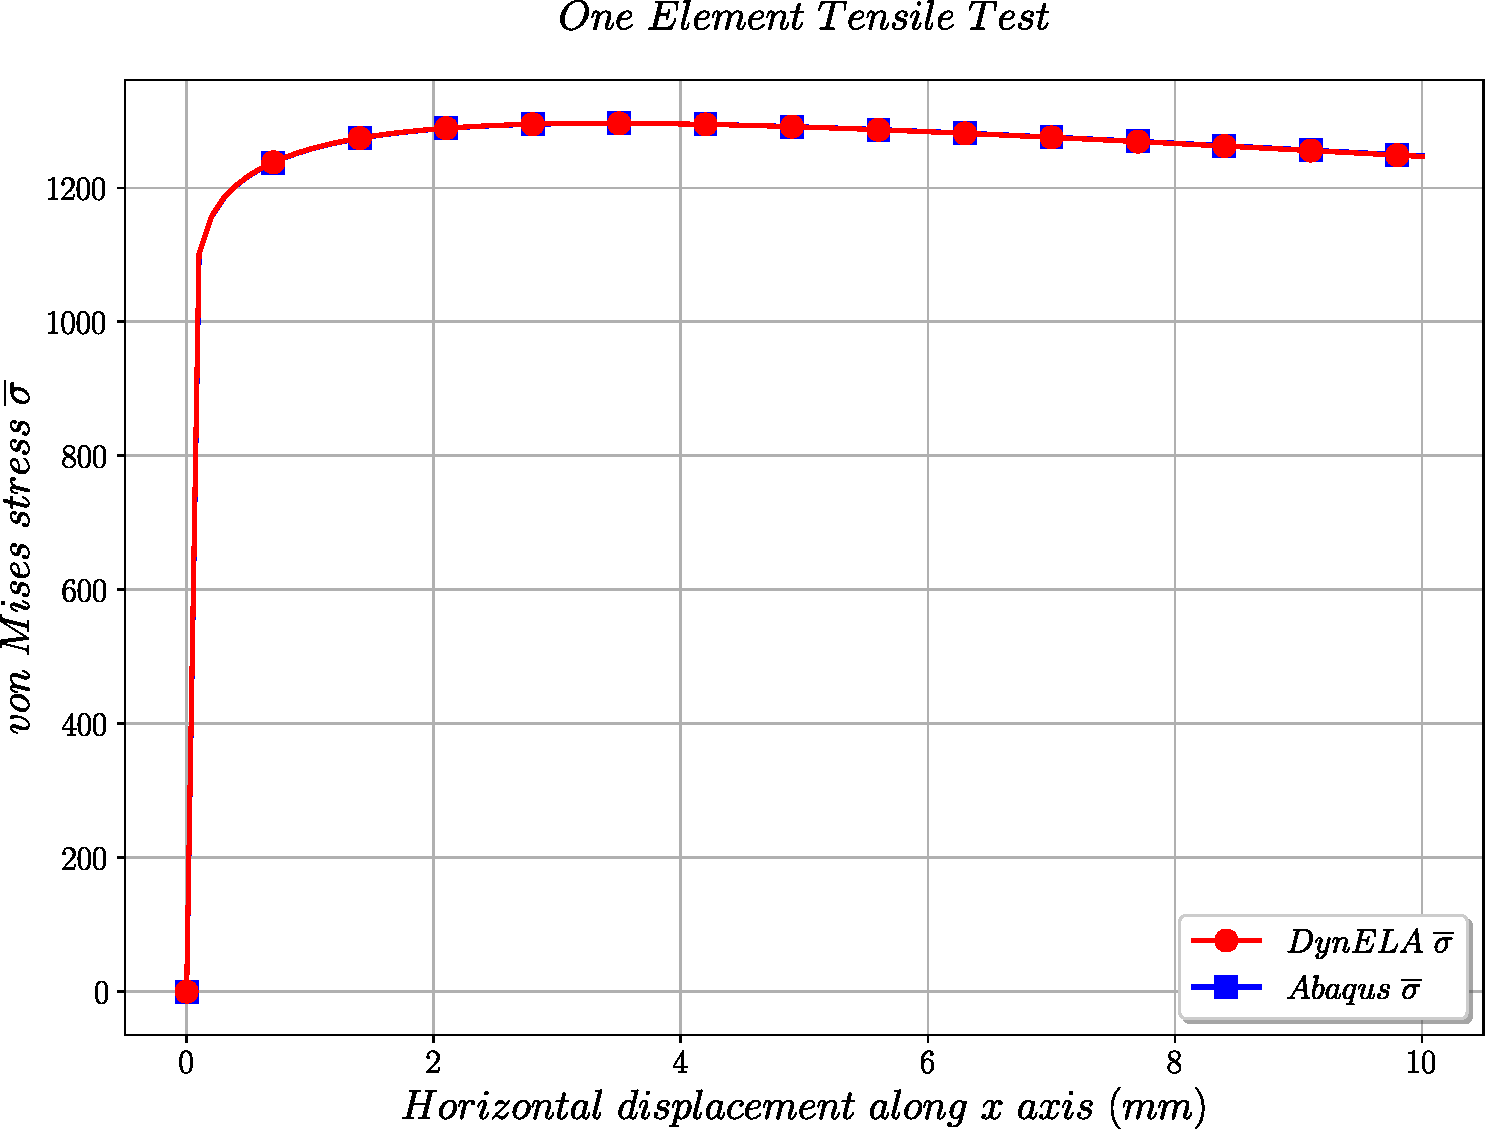
\includegraphics[width=0.45\columnwidth]{Figures/Samples/Element/Tensile3D_vonMises}\tabularnewline
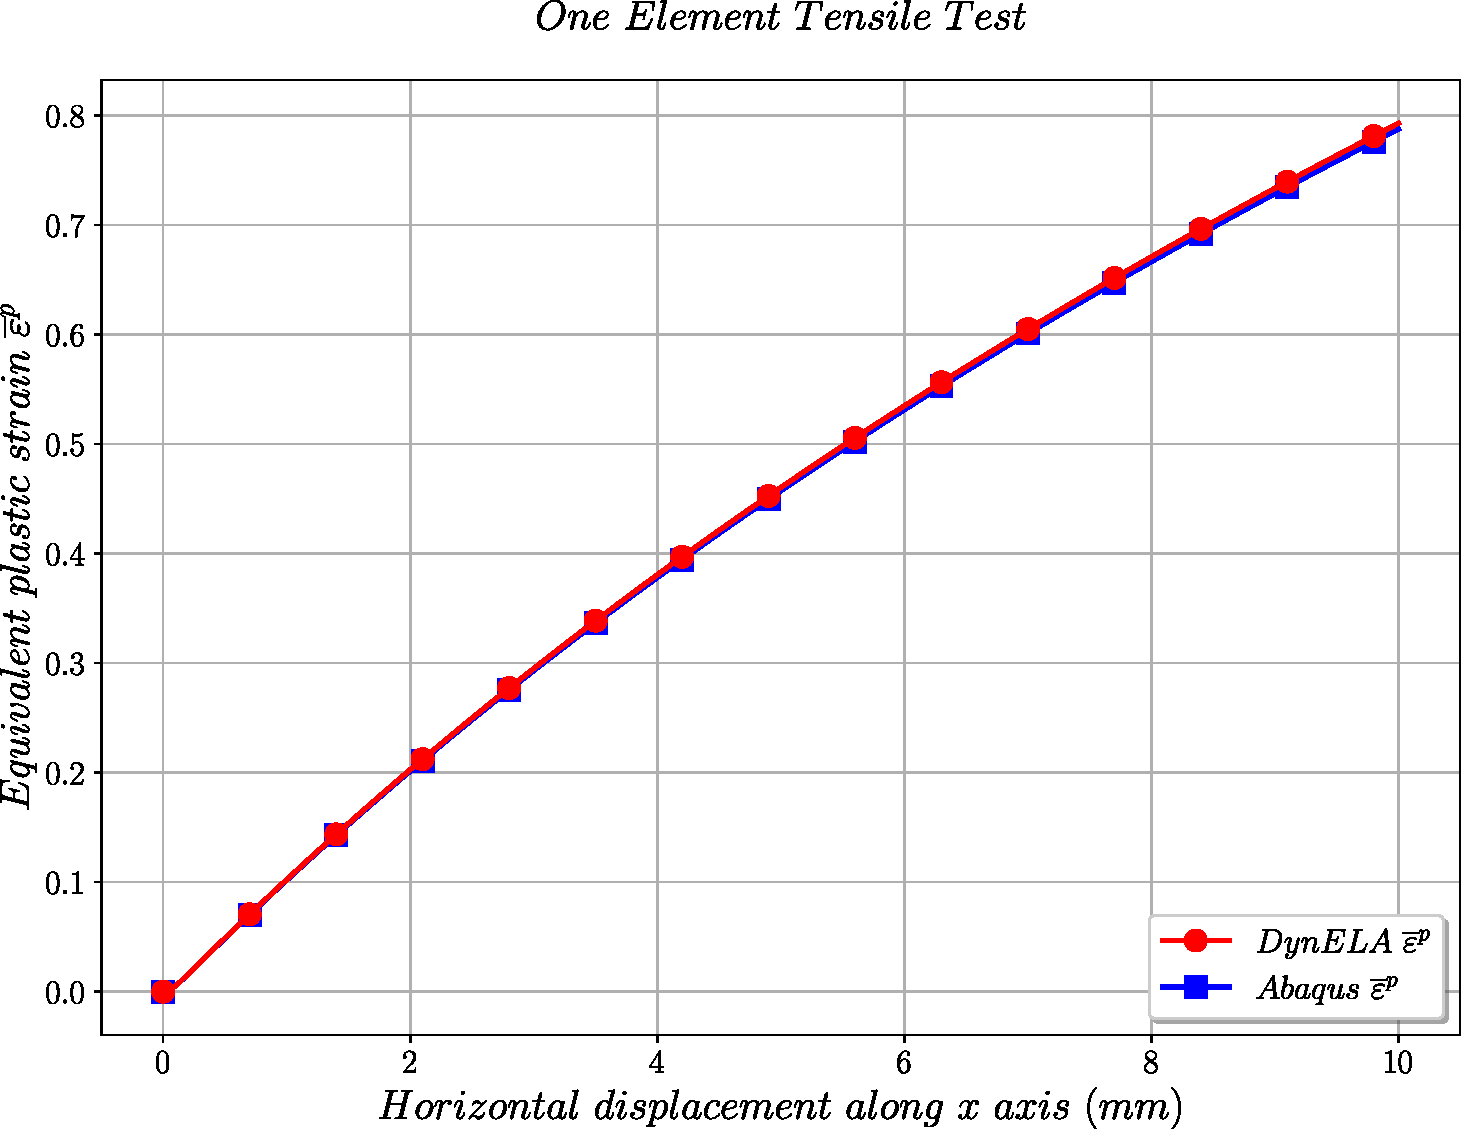
\includegraphics[width=0.45\columnwidth]{Figures/Samples/Element/Tensile3D_plasticStrain} & 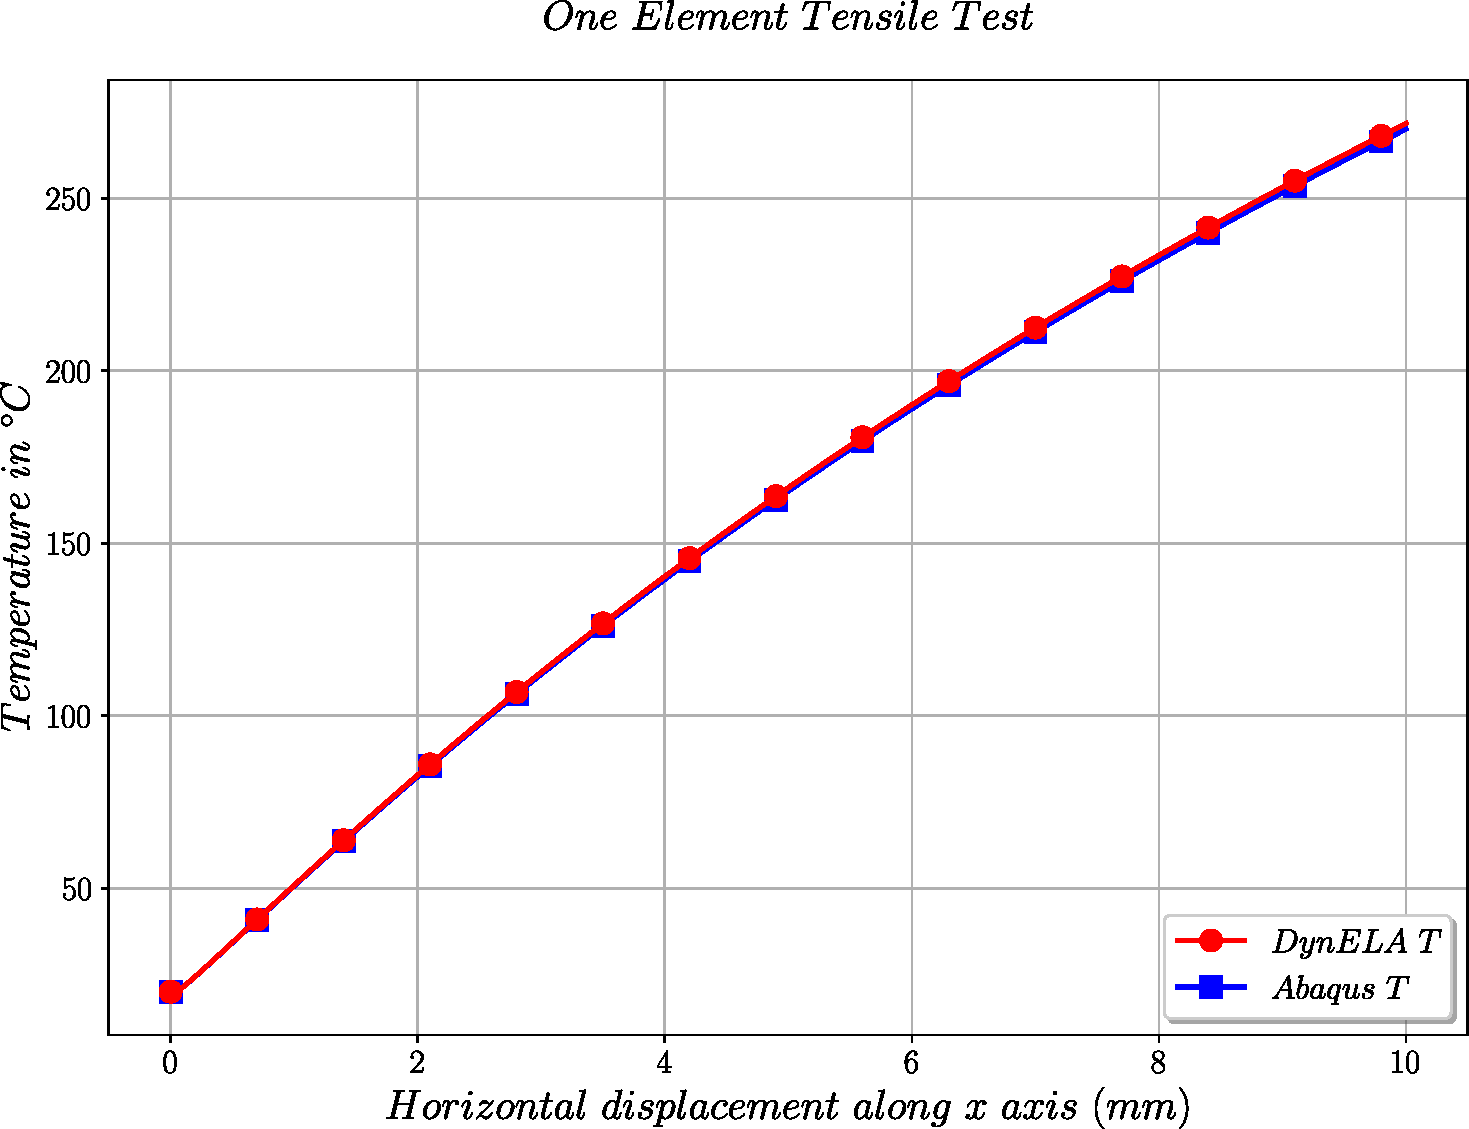
\includegraphics[width=0.45\columnwidth]{Figures/Samples/Element/Tensile3D_temperature}\tabularnewline
\end{tabular}
\par\end{centering}
\caption{Comparison of numerical and analytical results for the 3D one element
tensile test\label{fig:Samples!Single!Tensile-Comparison-3D}}
\end{figure}


\subsection{Element radial tensile test}

The uniaxial one element radial tensile test is a numerical test where
an axisymmetric element (with a square prescribed shape) is subjected
to pure radial tensile as presented in figure \ref{fig:Samples!Single!Tensile}.
The initial shape of the specimen is $10\,mm\times10\,mm$ and the
the two left nodes of the element are encastred and a prescribed horizontal
displacement $d=10\,mm$ is applied on the two right nodes of the
same element as illustrated in Figure \ref{fig:Samples!Single!Tensile}.
As we are using an explicit integration scheme, the total simulation
time is set to $t=0.01\,s$.

All the properties of the constitutive law reported in Table \ref{tab:Samples!JohnsonCookParameters}
are used and the material is assumed to follow the Johnson-Cook behavior
described by equation \ref{eq:Samples!Johnson-Cook}.

Figure \ref{fig:Samples!Single!Radial-Comparison} shows the comparison
of the DynELA solver results (plotted in red) and the Abaqus numerical
results (plotted in blue) concerning the evolution of the stress components
$\sigma_{11}$, $\sigma_{22}$, $\sigma_{12}$, $\overline{\sigma}$,
$\overline{\varepsilon}^{p}$ and $T$ \versus  the horizontal displacement
of the right edge of the specimen along the horizontal axis. Again,
comparison of Abaqus and DynELA results is made by averaging the DynELA
results on the $4$ integration points of the element because \DynELA uses
full integrated elements while Abaqus have reduced integrated elements
only but in fact, the DynELA results at the $4$ integration points
are the same in this benchmark test.

\begin{figure}[h]
\begin{centering}
\begin{tabular}{cc}
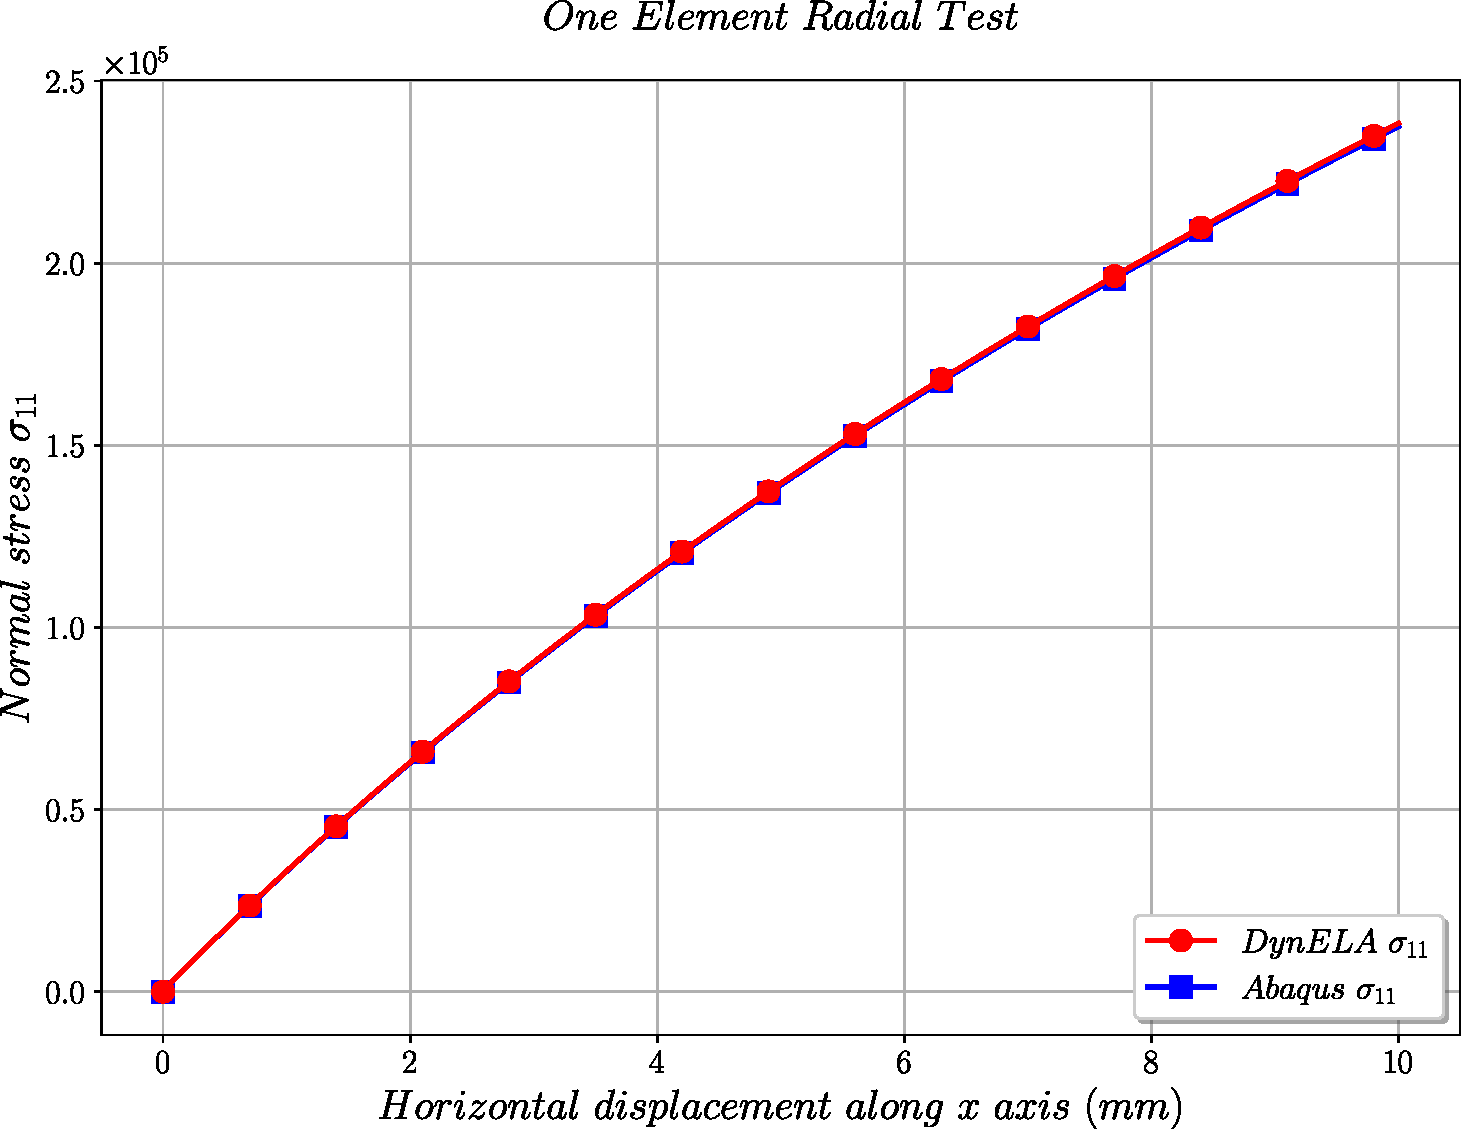
\includegraphics[width=0.45\columnwidth]{Figures/Samples/Element/Radial_stress_11} & 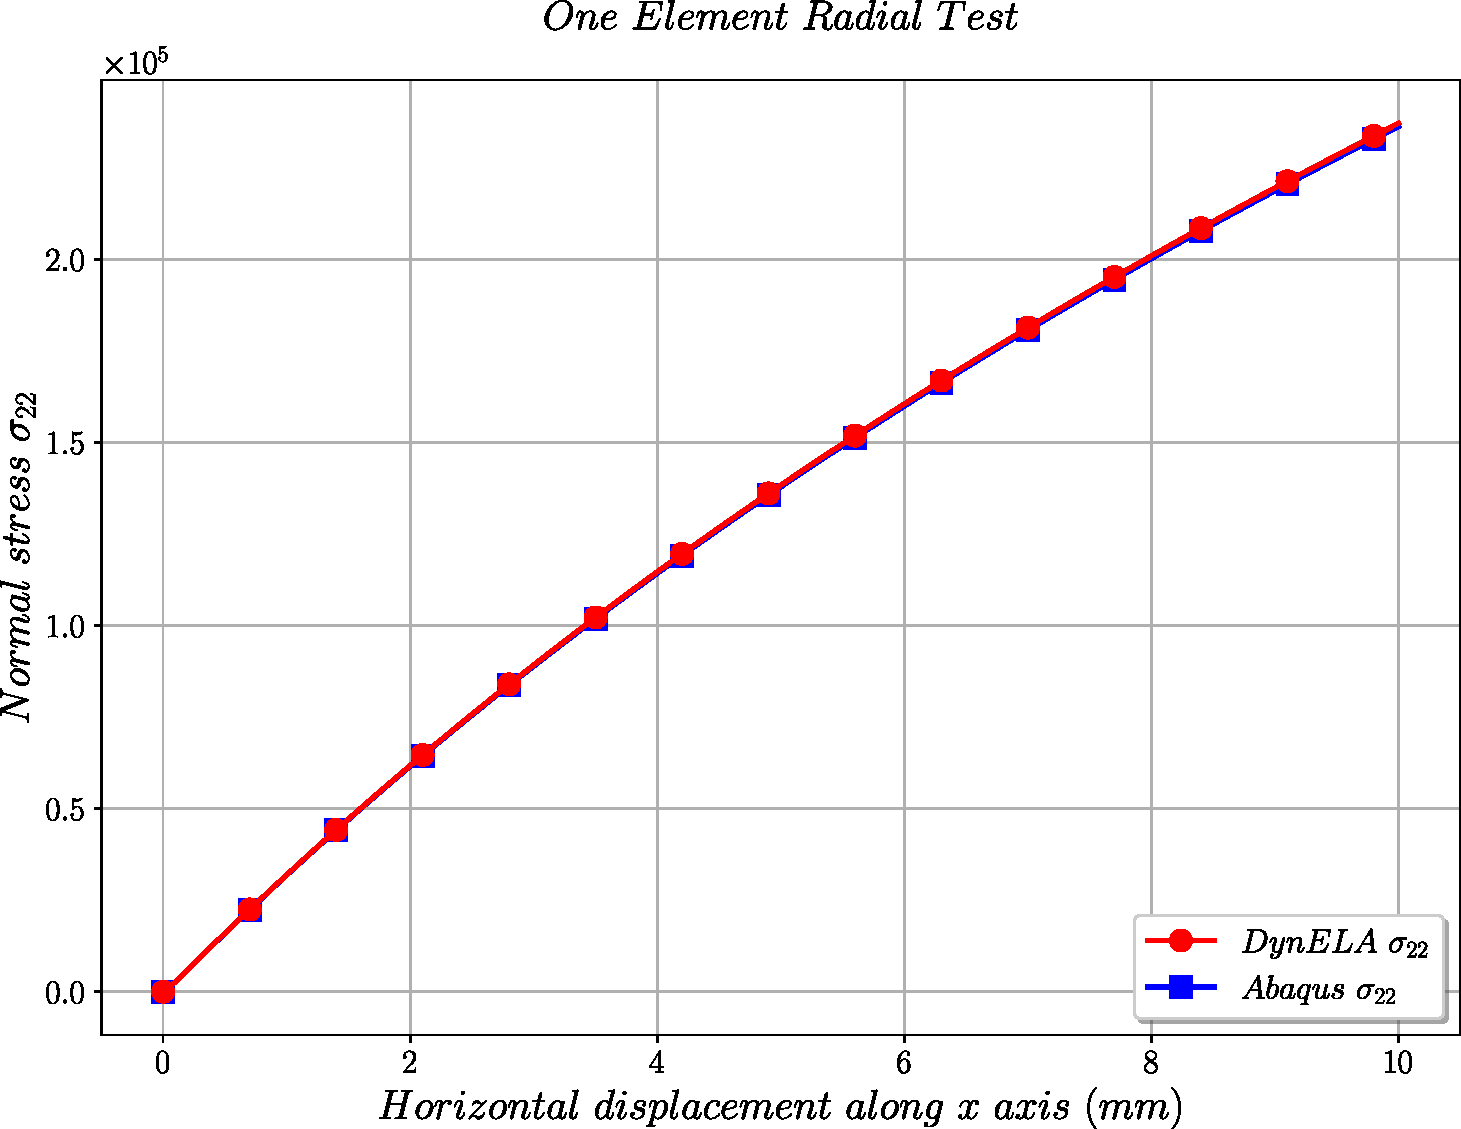
\includegraphics[width=0.45\columnwidth]{Figures/Samples/Element/Radial_stress_22}\tabularnewline
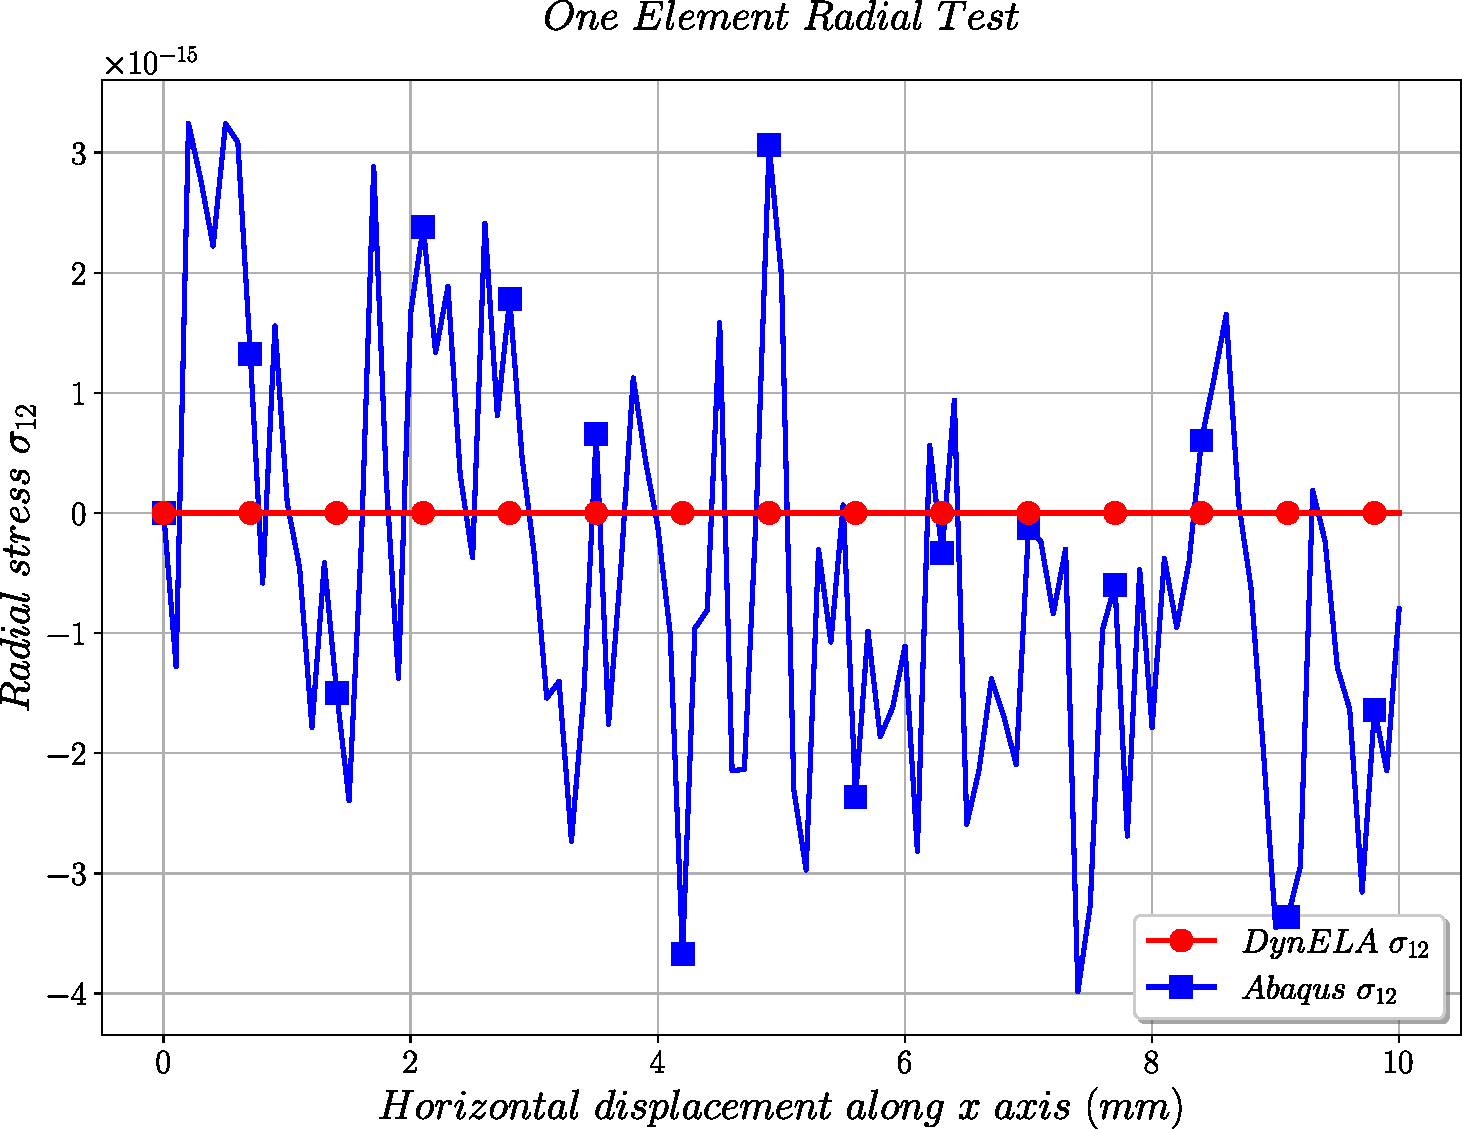
\includegraphics[width=0.45\columnwidth]{Figures/Samples/Element/Radial_stress_12} & 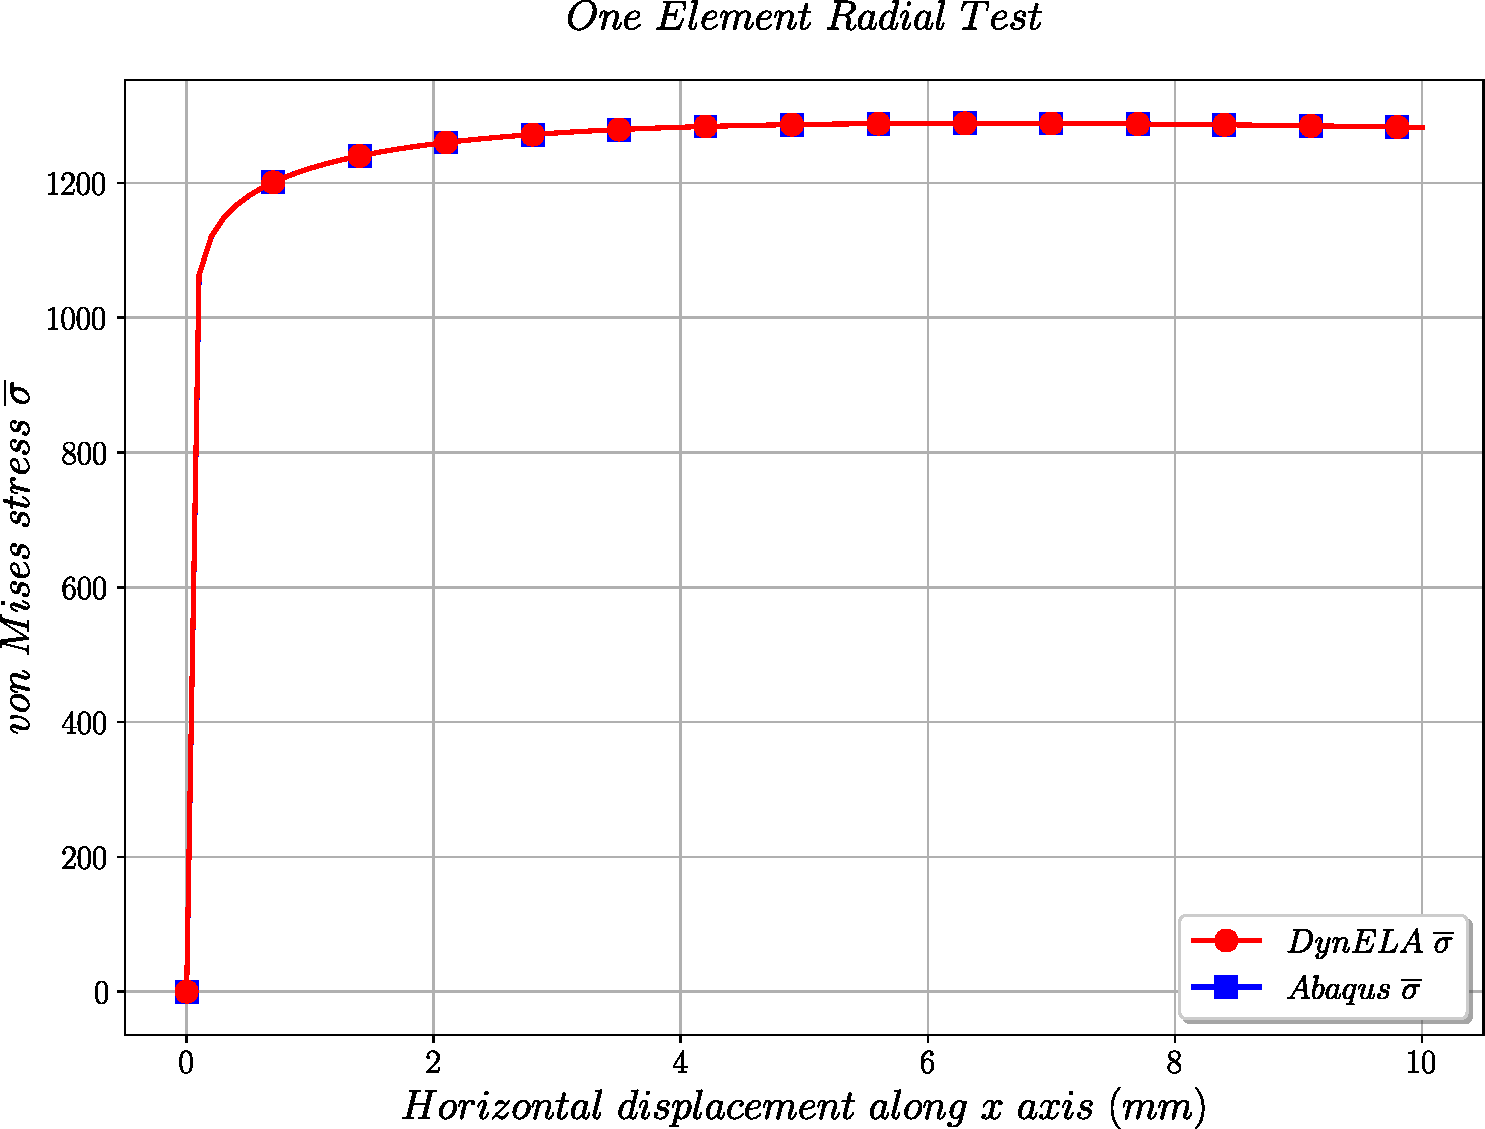
\includegraphics[width=0.45\columnwidth]{Figures/Samples/Element/Radial_vonMises}\tabularnewline
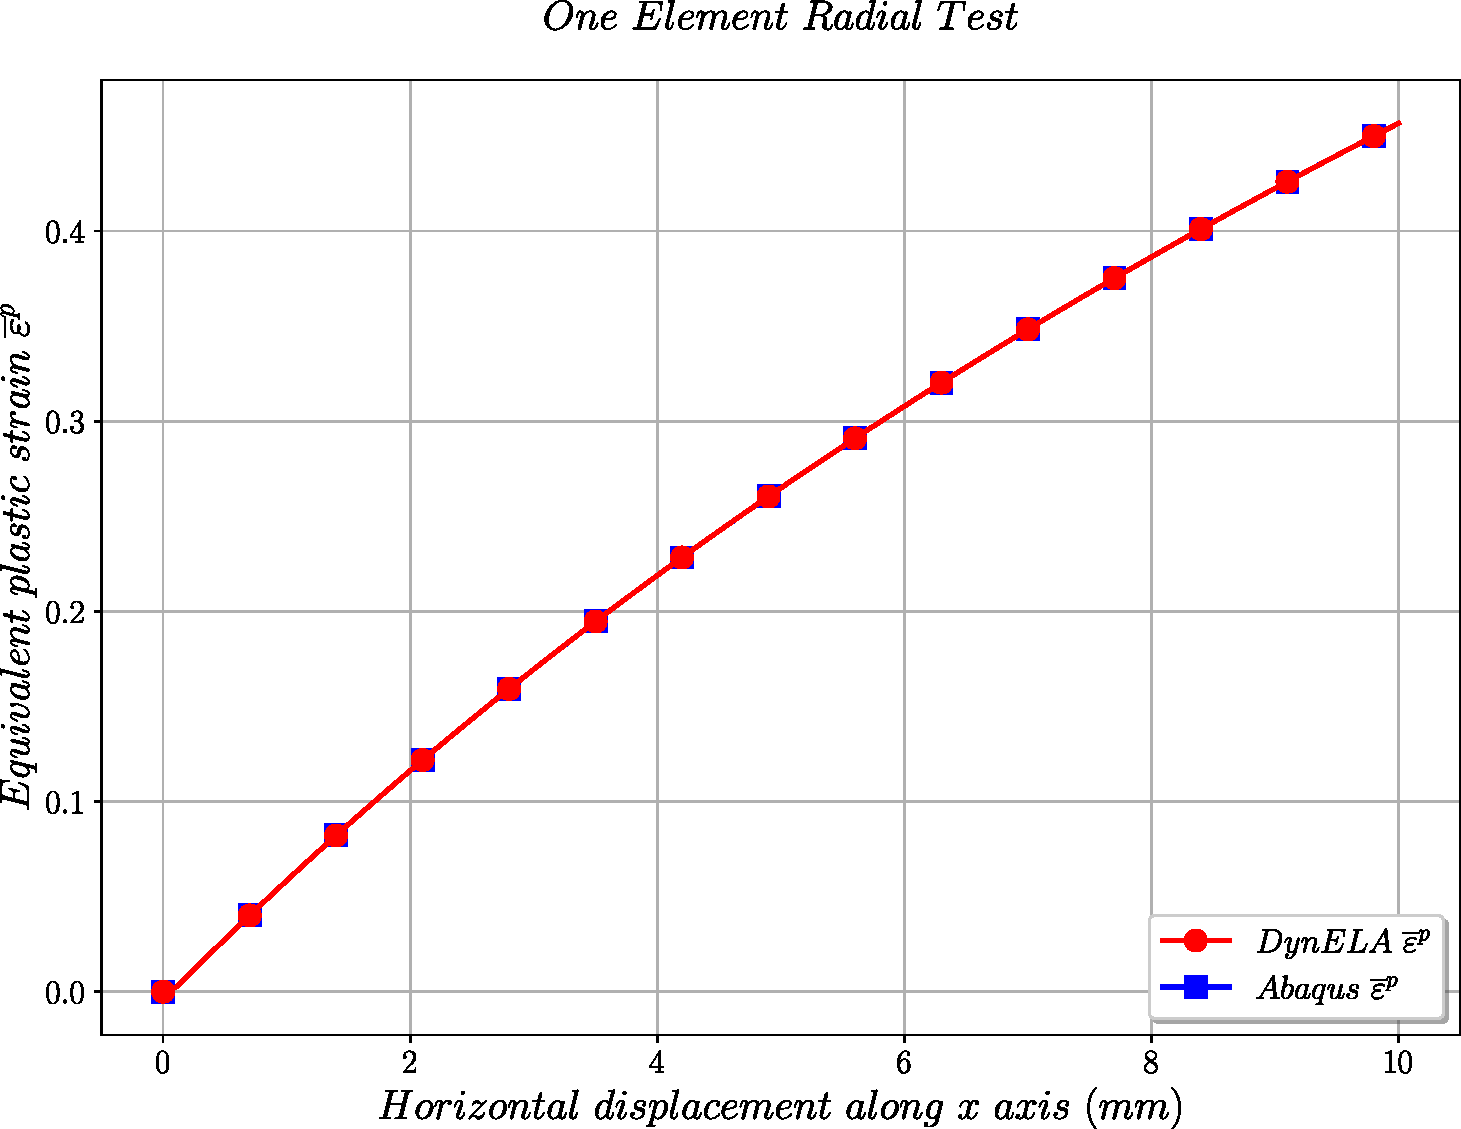
\includegraphics[width=0.45\columnwidth]{Figures/Samples/Element/Radial_plasticStrain} & 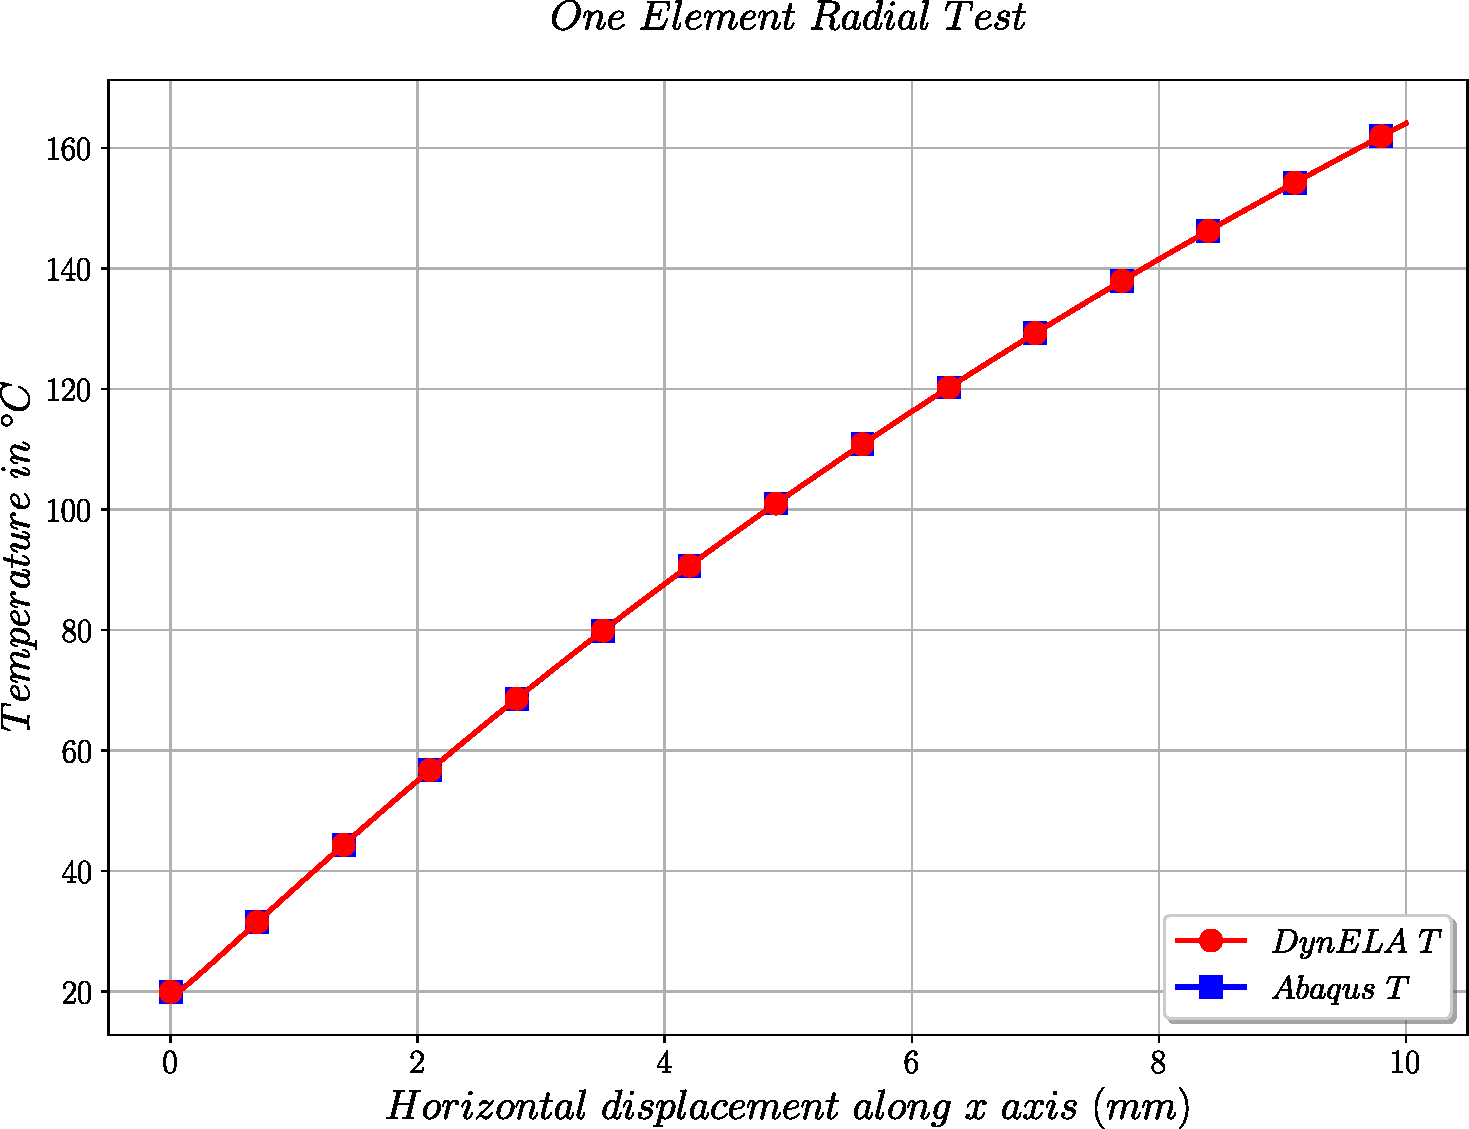
\includegraphics[width=0.45\columnwidth]{Figures/Samples/Element/Radial_temperature}\tabularnewline
\end{tabular}
\par\end{centering}
\caption{Comparison of numerical and analytical results for the one element
radial tensile test\label{fig:Samples!Single!Radial-Comparison}}
\end{figure}
\clearpage

\subsection{Element radial torus test}

The uniaxial one element torus tensile test is a numerical test where
an axisymmetric element (with a square prescribed shape) is subjected
to radial tensile as presented in figure \ref{fig:Samples!Single!Torus}.
\begin{figure}[h]
\begin{centering}
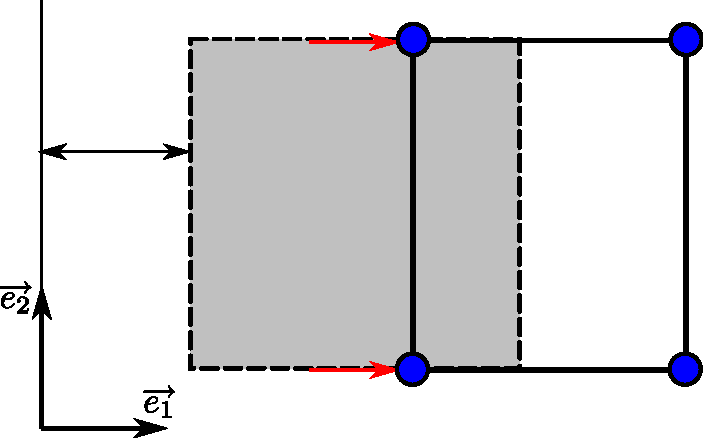
\includegraphics[width=0.5\columnwidth]{Figures/SamplesSingleTorus}
\par\end{centering}
\caption{Numerical model for the one element torus test\label{fig:Samples!Single!Torus}}
\end{figure}
 The difference with the previous test is that the left edge of the
specimen in not aligned with the symmetry axis, the radial coordinate
of the left edge is $r=10\,mm$. The initial shape of the specimen
is $10\,mm\times10\,mm$ and a prescribed horizontal displacement
$d=10\,mm$ is applied on the two left nodes of the element as illustrated
in Figure \ref{fig:Samples!Single!Torus}. As we are using an explicit
integration scheme, the total simulation time is set to $t=0.01\,s$.
All the properties of the constitutive law reported in Table \ref{tab:Samples!JohnsonCookParameters}
are used and the material is assumed to follow the Johnson-Cook behavior
described by equation \ref{eq:Samples!Johnson-Cook}.

As a global comparison, Figure \ref{fig:Samples!Single!Torus-Comparison-ux}
show the comparison of the right edge displacement \versus the left
edge displacement for both the DynELA and the Abaqus simulations.
\begin{figure}[h]
\begin{centering}
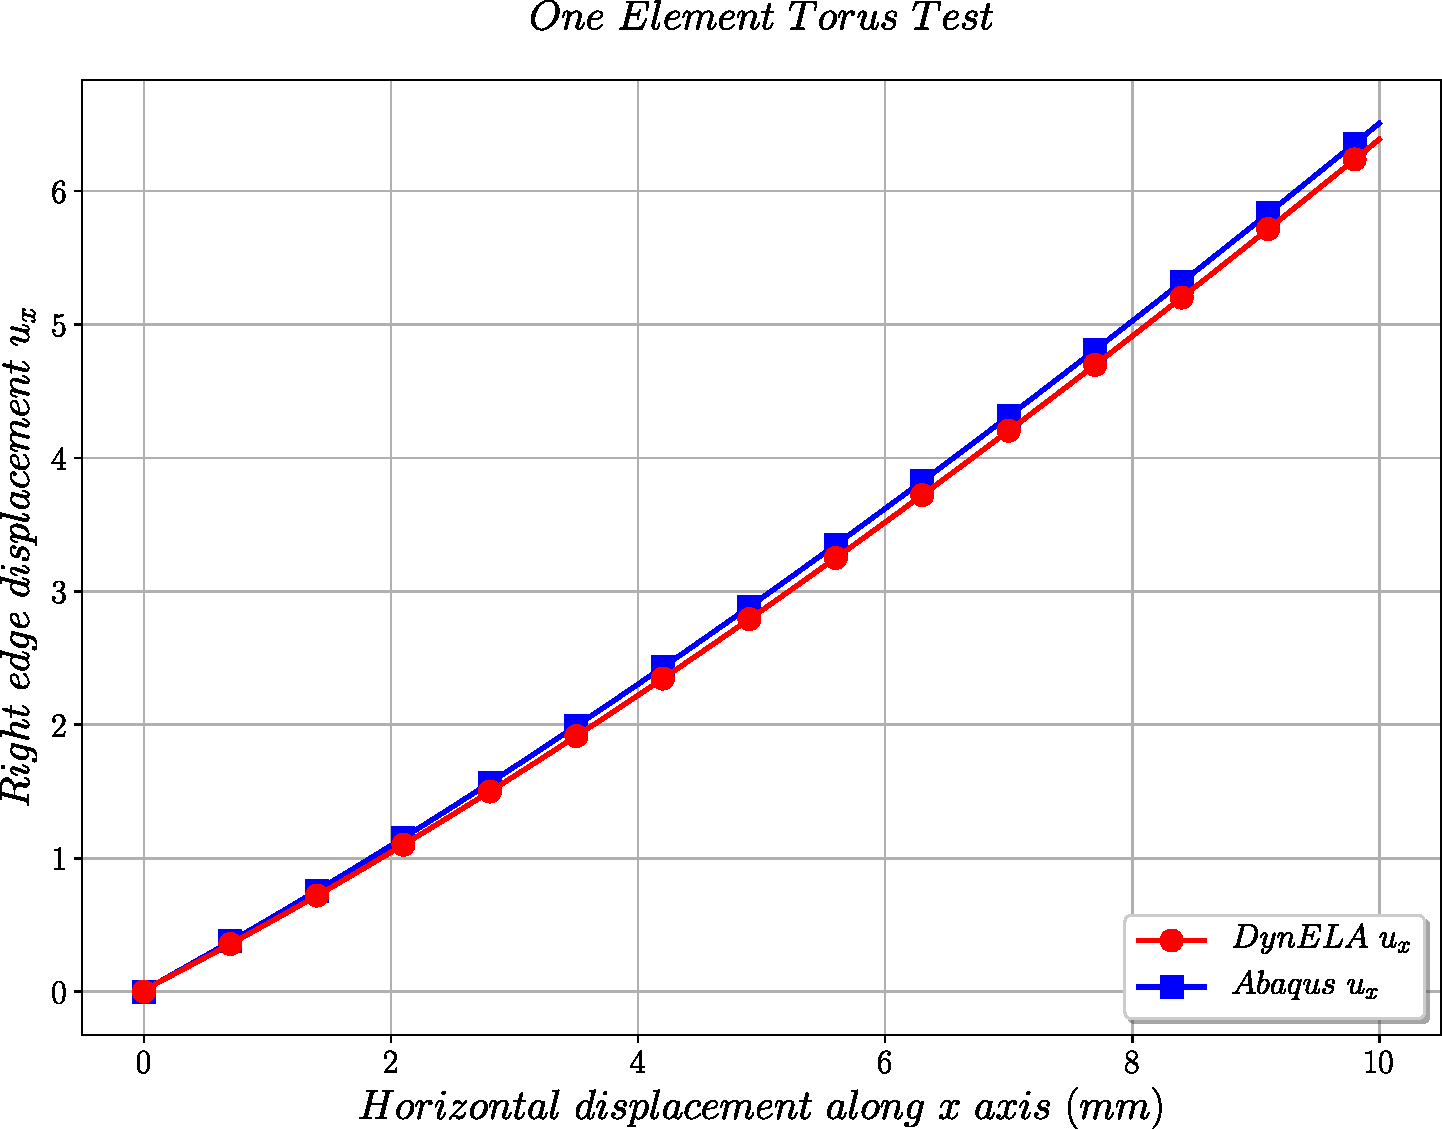
\includegraphics[width=0.5\columnwidth]{Figures/Samples/Element/Torus_dispX}
\par\end{centering}
\caption{Comparison of the right edge displacement for the one element torus
test\label{fig:Samples!Single!Torus-Comparison-ux}}
\end{figure}

Figure \ref{fig:Samples!Single!Torus-Comparison} shows the comparison
of the DynELA solver results (plotted in red) and the Abaqus numerical
results (plotted in blue) concerning the evolution of the stress components
$\sigma_{11}$, $\sigma_{22}$, $\sigma_{12}$, $\overline{\sigma}$,
$\overline{\varepsilon}^{p}$ and $T$ \versus  the horizontal displacement
of the right edge of the specimen along the horizontal axis. As the
Abaqus software only provides under-integrated elements, we are using
a $2\times2$ elements mesh for the Abaqus model, as presented in
Figure \ref{fig:Samples!Single!Torus-Abaqus}, to compare the results.
On abaqus, the mean value of the results of the $4$ elements is computed
and compared to the mean value of the $4$ integration points of the
DynELA simulation.
\begin{figure}[h]
\begin{centering}
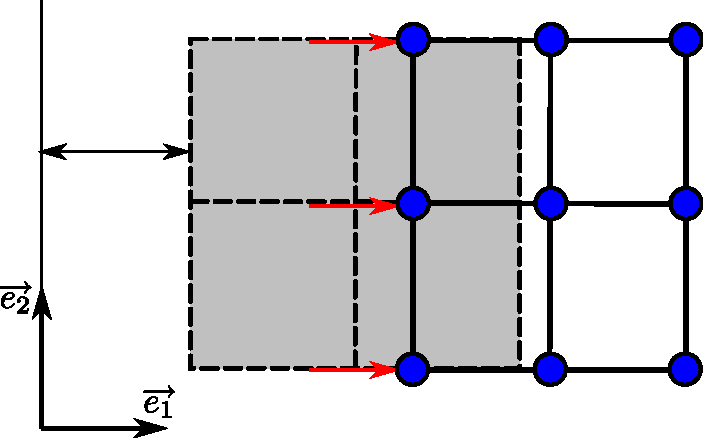
\includegraphics[width=0.5\columnwidth]{Figures/SamplesSingleTorusAbaqus}
\par\end{centering}
\caption{Numerical model for the one element torus test under Abaqus\label{fig:Samples!Single!Torus-Abaqus}}
\end{figure}

\begin{figure}[h]
\begin{centering}
\begin{tabular}{cc}
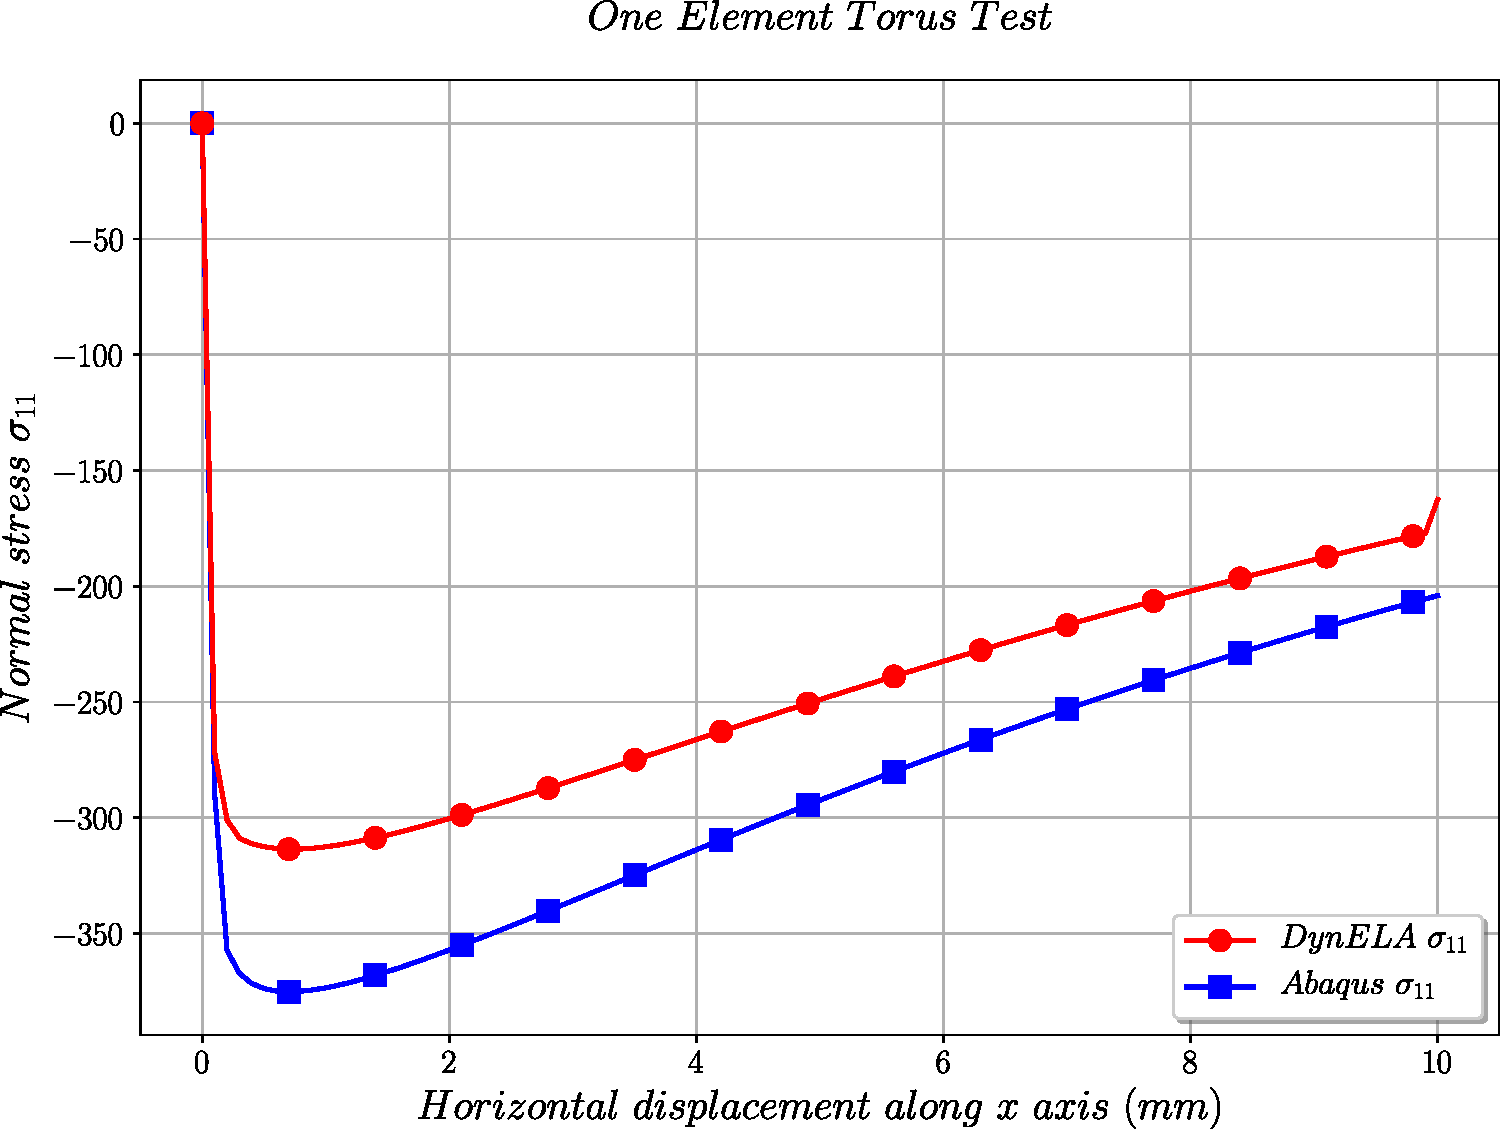
\includegraphics[width=0.45\columnwidth]{Figures/Samples/Element/Torus_stress_11} & 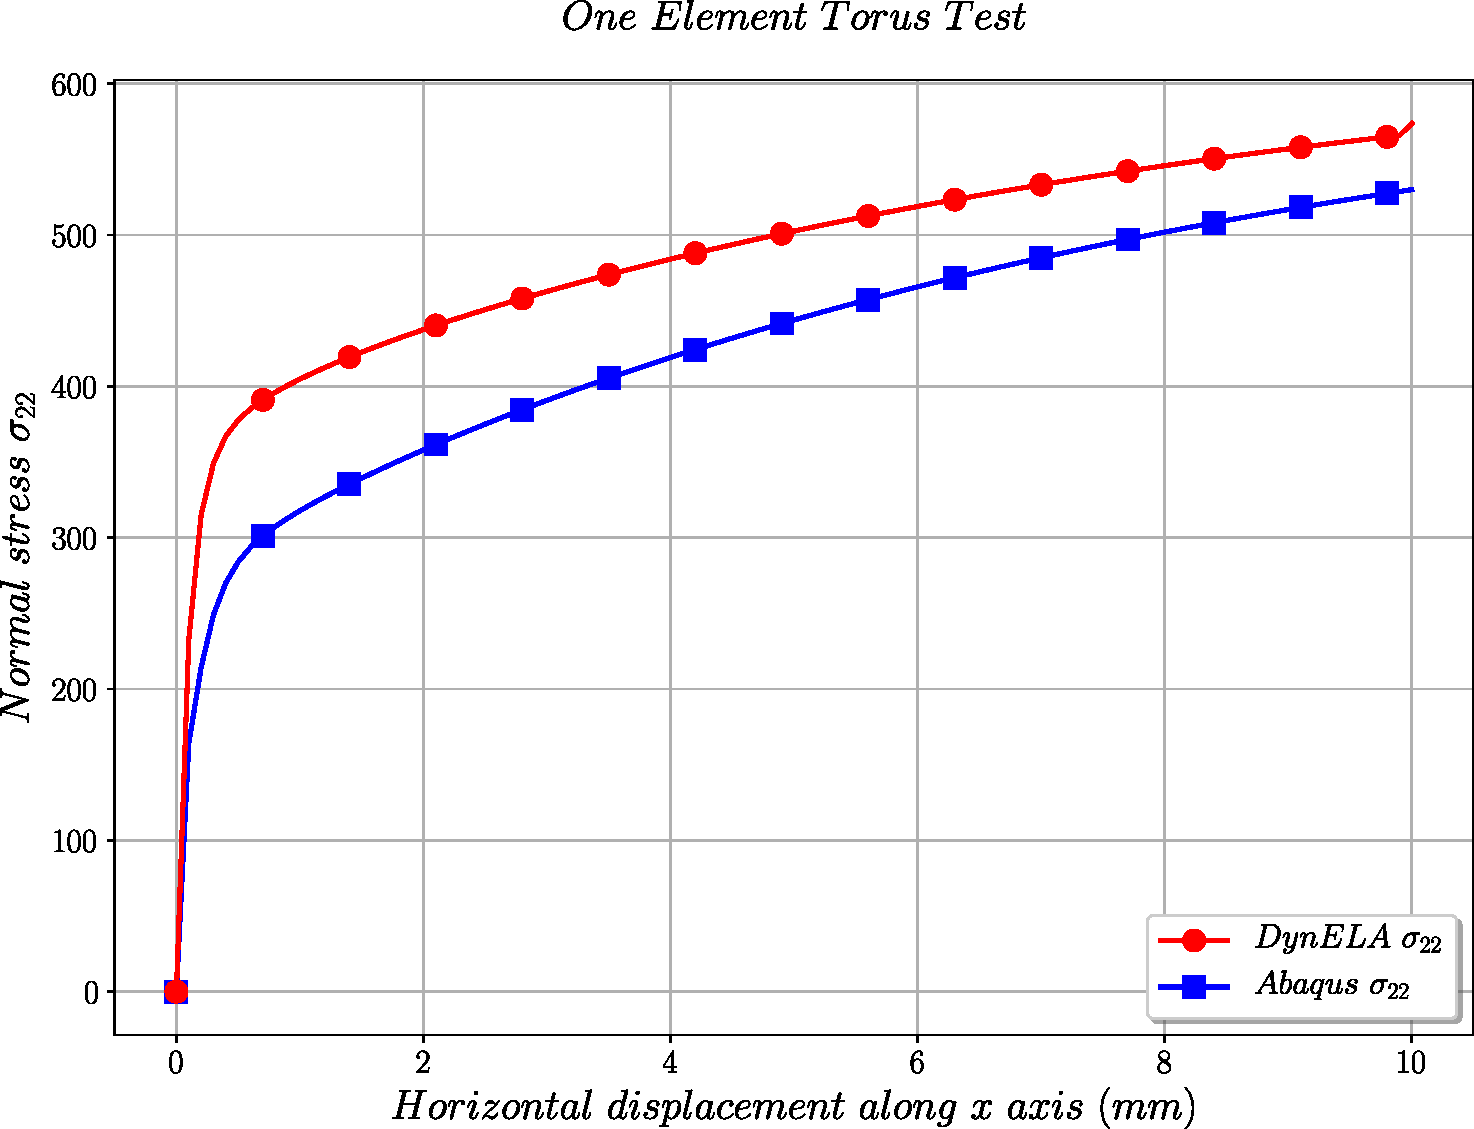
\includegraphics[width=0.45\columnwidth]{Figures/Samples/Element/Torus_stress_22}\tabularnewline
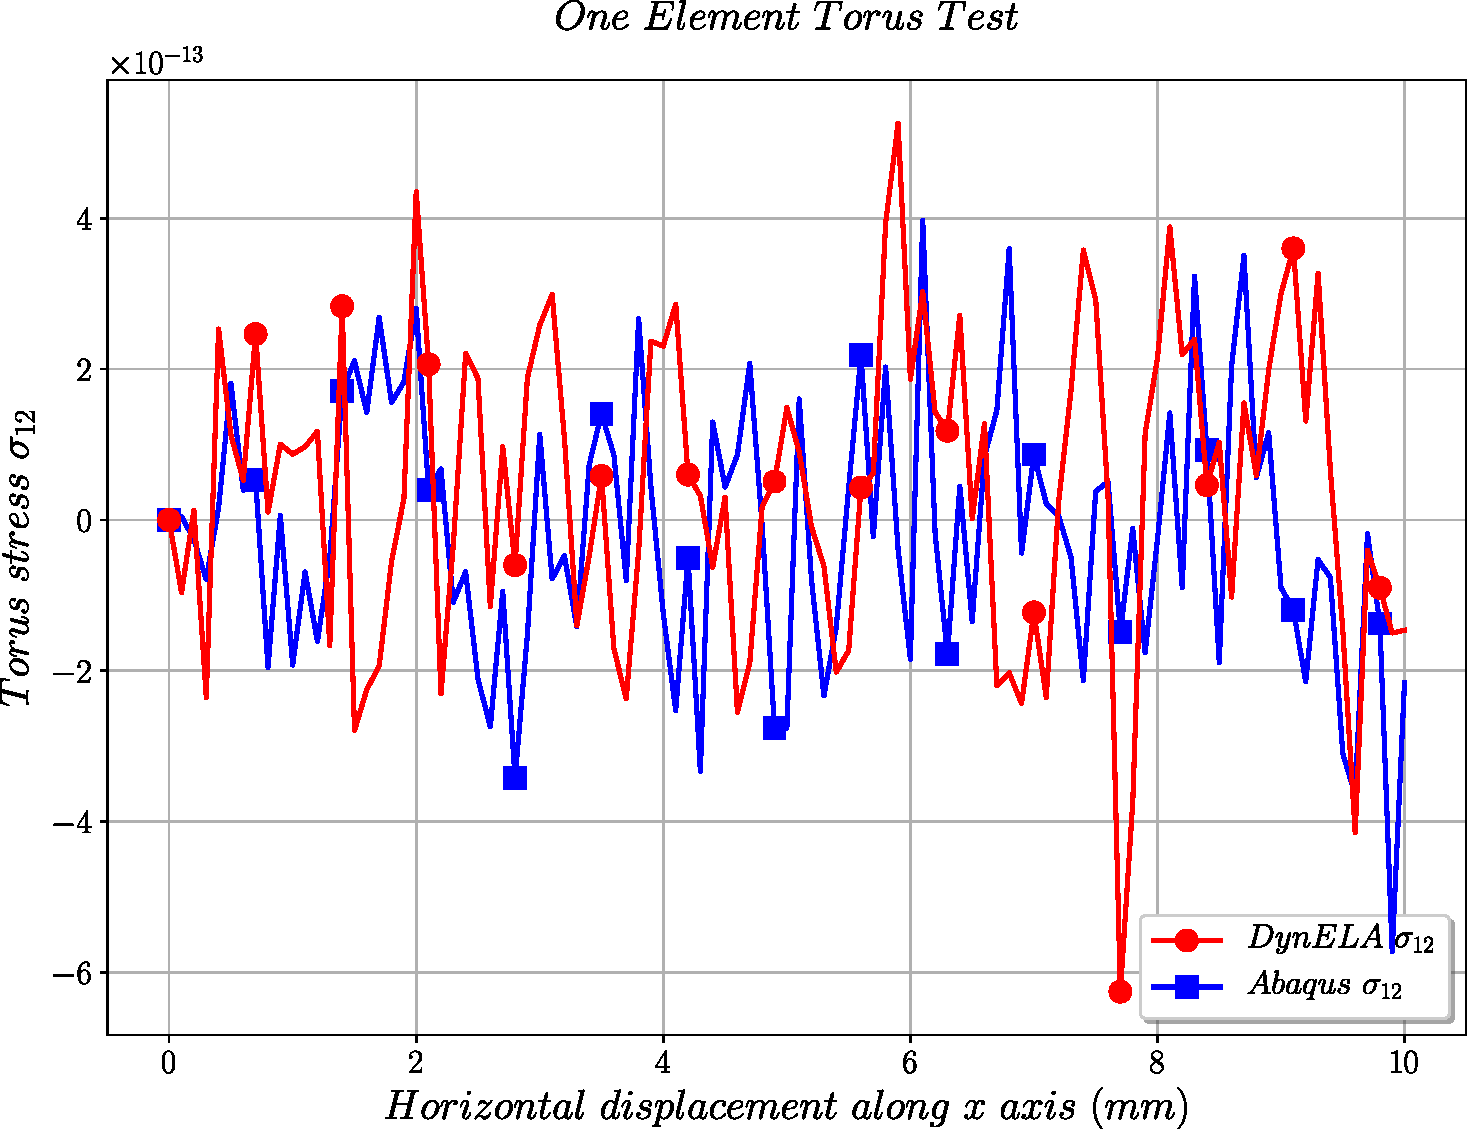
\includegraphics[width=0.45\columnwidth]{Figures/Samples/Element/Torus_stress_12} & 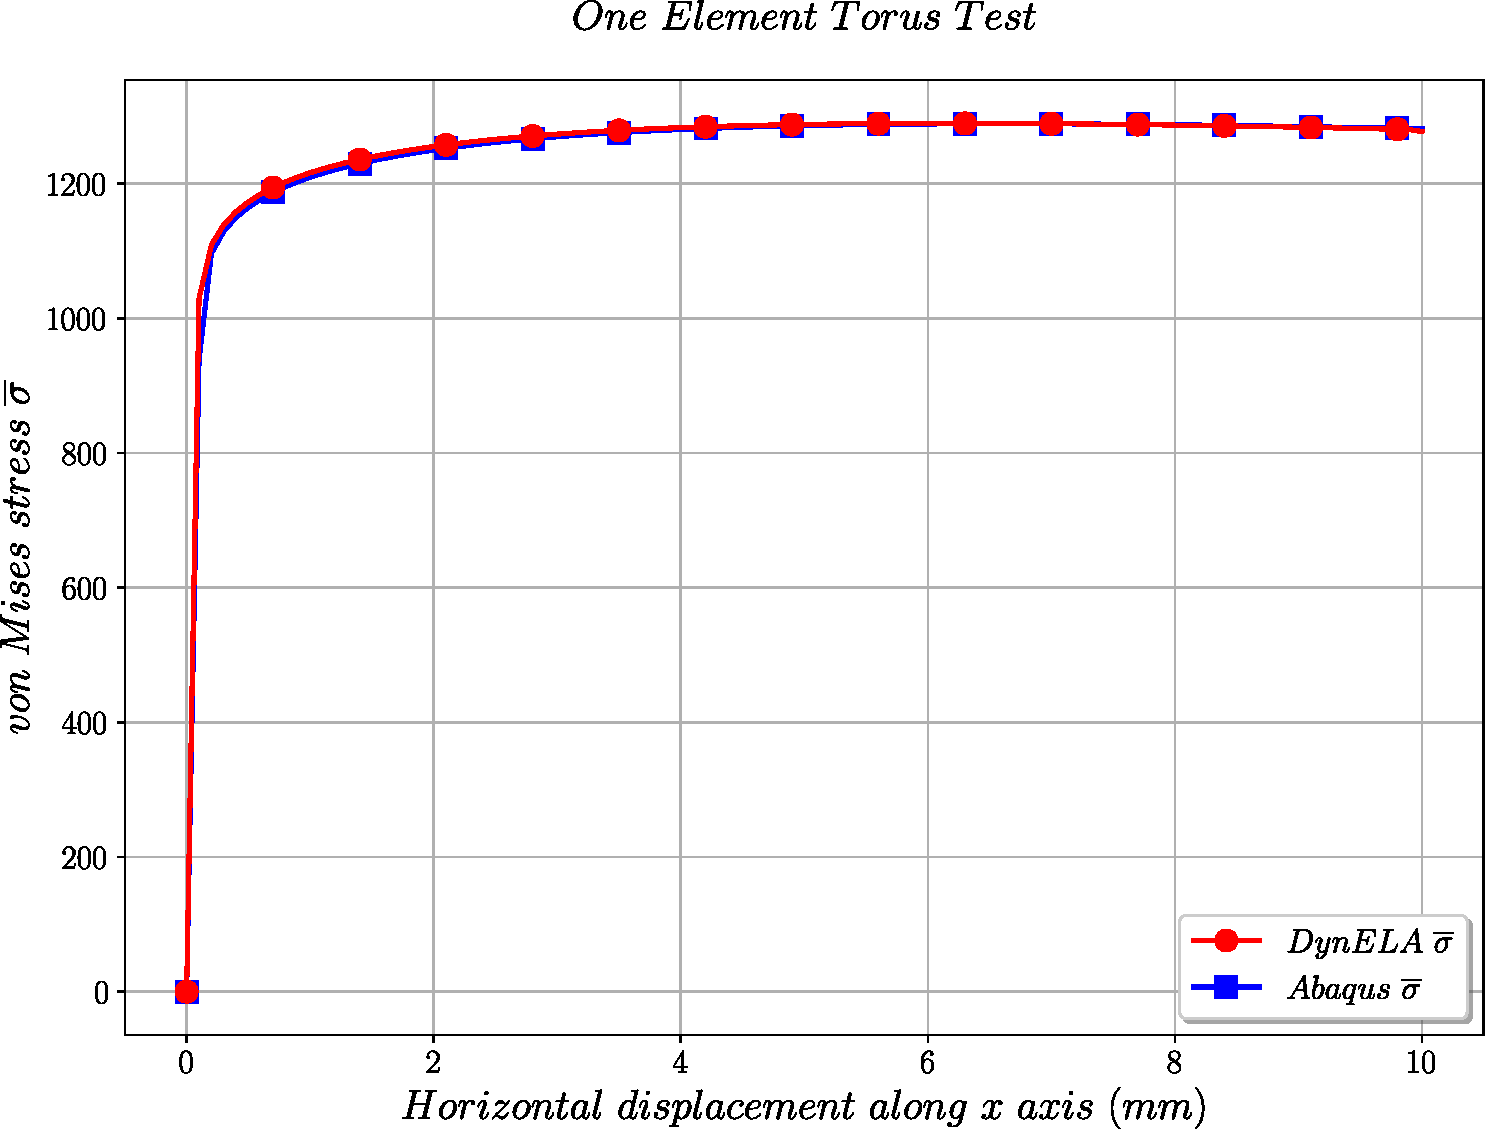
\includegraphics[width=0.45\columnwidth]{Figures/Samples/Element/Torus_vonMises}\tabularnewline
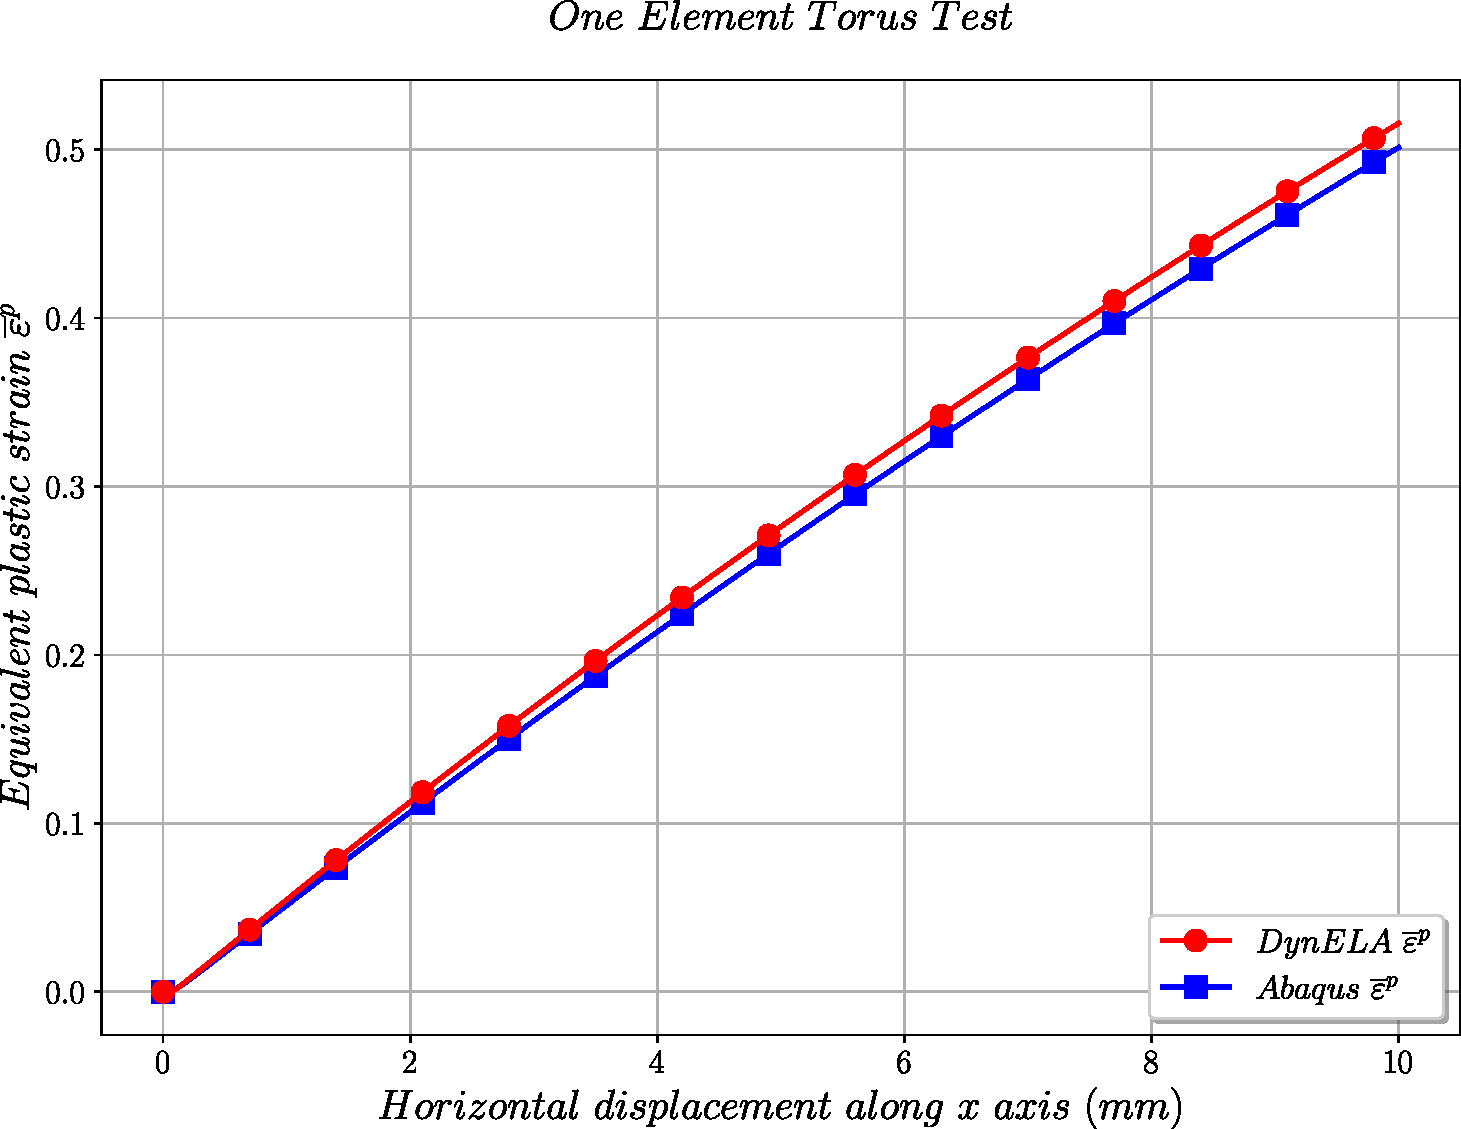
\includegraphics[width=0.45\columnwidth]{Figures/Samples/Element/Torus_plasticStrain} & 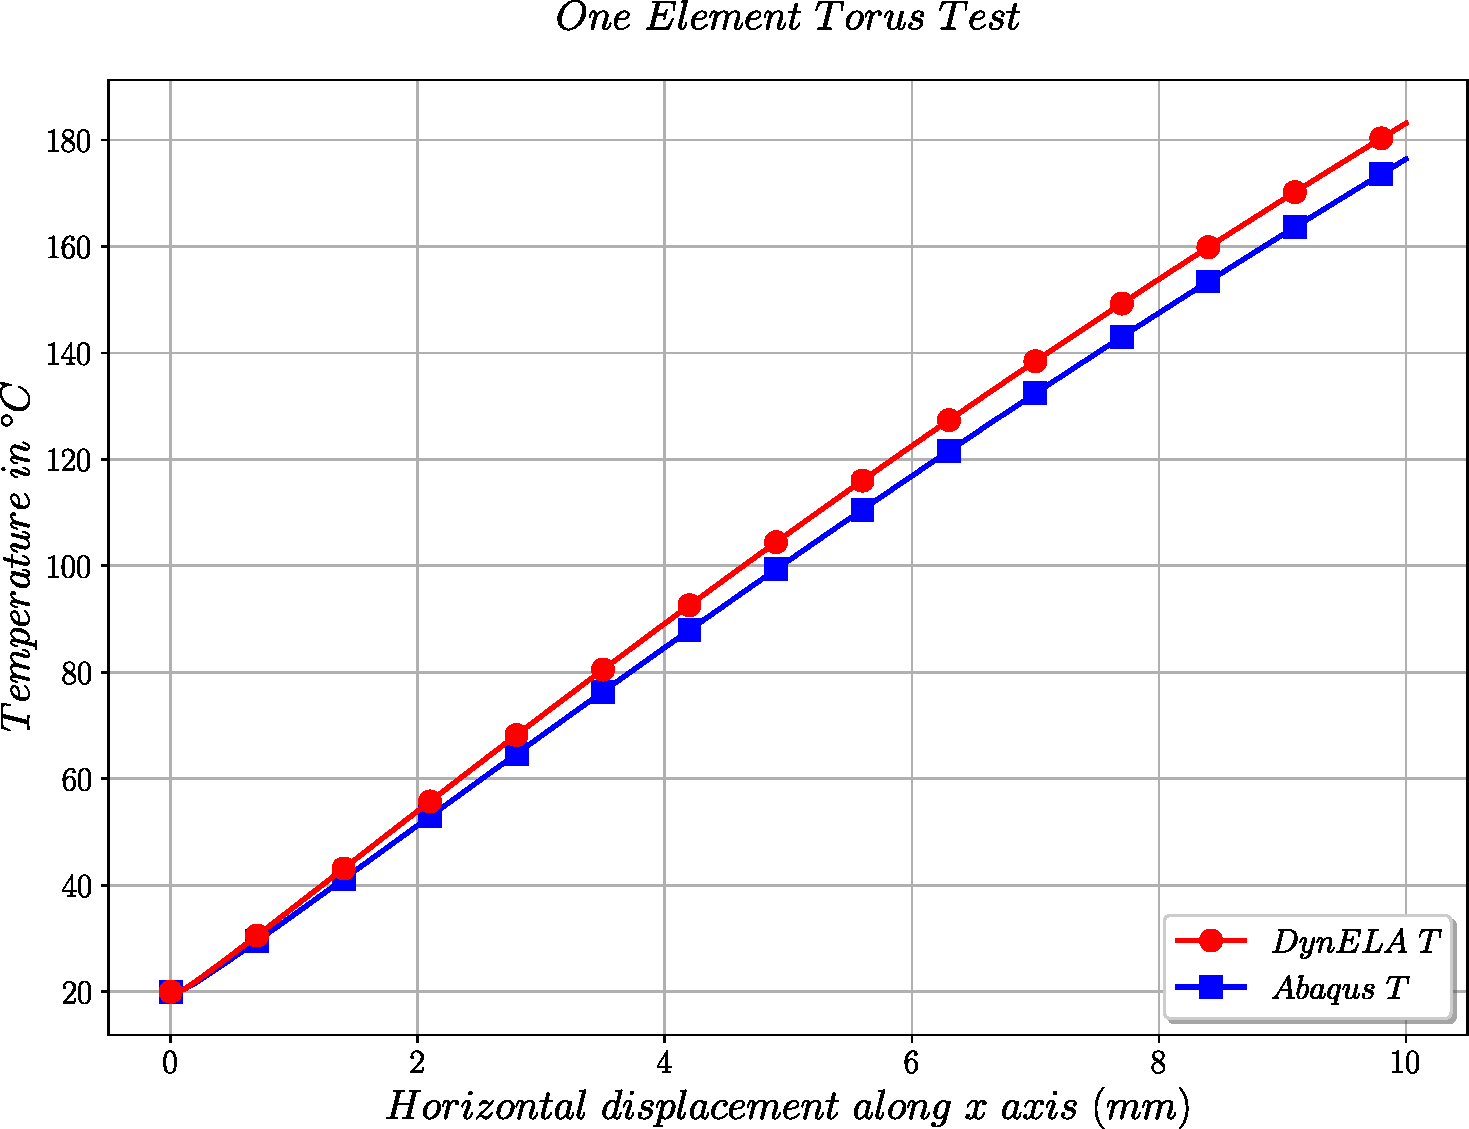
\includegraphics[width=0.45\columnwidth]{Figures/Samples/Element/Torus_temperature}\tabularnewline
\end{tabular}
\par\end{centering}
\caption{Comparison of numerical results for the one element torus tensile
test\label{fig:Samples!Single!Torus-Comparison}}
\end{figure}
\clearpage

\section{Uniaxial one element shear test}

The uniaxial one element shear test is a numerical test where an element
(with a square prescribed shape) is subjected to pure shear test as
presented in figure \ref{fig:Samples!Single!Shear}.
\begin{figure}[h]
\begin{centering}
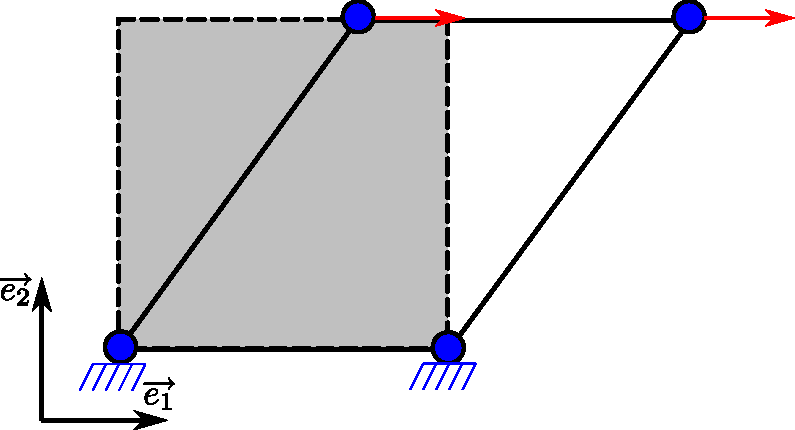
\includegraphics[width=0.5\columnwidth]{Figures/SamplesSingleShear}
\par\end{centering}
\caption{Numerical model for the one element shear test\label{fig:Samples!Single!Shear}}
\end{figure}
 The initial shape of the specimen is $10\,mm\times10\,mm$ and the
the two bottom nodes of the element are encastred and a prescribed
horizontal displacement $d=100\,mm$ is applied on the two upper nodes
of the same element as illustrated in Figure \ref{fig:Samples!Single!Shear}.
As we are using an explicit integration scheme, the total simulation
time is set to $t=0.01\,s$. Mechanical properties of the material
are reported in Table \ref{tab:Samples!JohnsonCookParameters}.

Comparison of Abaqus and DynELA results is made by averaging the DynELA
results on the $4$ integration points of the element. This has been
done because \DynELA uses full integrated elements while Abaqus
have reduced integrated elements only but in fact, the DynELA results
at the $4$ integration points are the same in this benchmark test.

\subsection{Elastic case}

In this case, only the elastic properties of the constitutive law
reported in Table \ref{tab:Samples!JohnsonCookParameters} are used
and the material is assumed to be hyper-elastic. As we are using a
Jaumann objective rate within the \DynELA, one can obtain, using
an analytical development, the following results for the proposed
case:
\begin{equation}
\Sig=G\left[\begin{array}{ccc}
1-\cos e & \sin e & 0\\
 & \cos e-1 & 0\\
sym &  & 0
\end{array}\right],
\end{equation}
where $G=\mu=\frac{E}{2(1+\nu)}$ is the shear modulus of the material
and $e$ is the elongation along the horizontal axis with $e_{max}=10$
conforming to the prescribed boundaries conditions. Figure \ref{fig:Samples!Single!Shear-Elastic-Comparison}
shows the comparison of the DynELA solver results (plotted in red)
and both the analytical (plotted in blue) and the Abaqus numerical
results (plotted in green) concerning the evolution of the stress
components $\sigma_{11}$, $\sigma_{22}$, $\sigma_{12}$ and $\overline{\sigma}$
\versus  the horizontal displacement of the top edge of the specimen
along the horizontal axis. A perfect match between all those results
can be seen from this later.

\begin{figure}[h]
\begin{centering}
\begin{tabular}{cc}
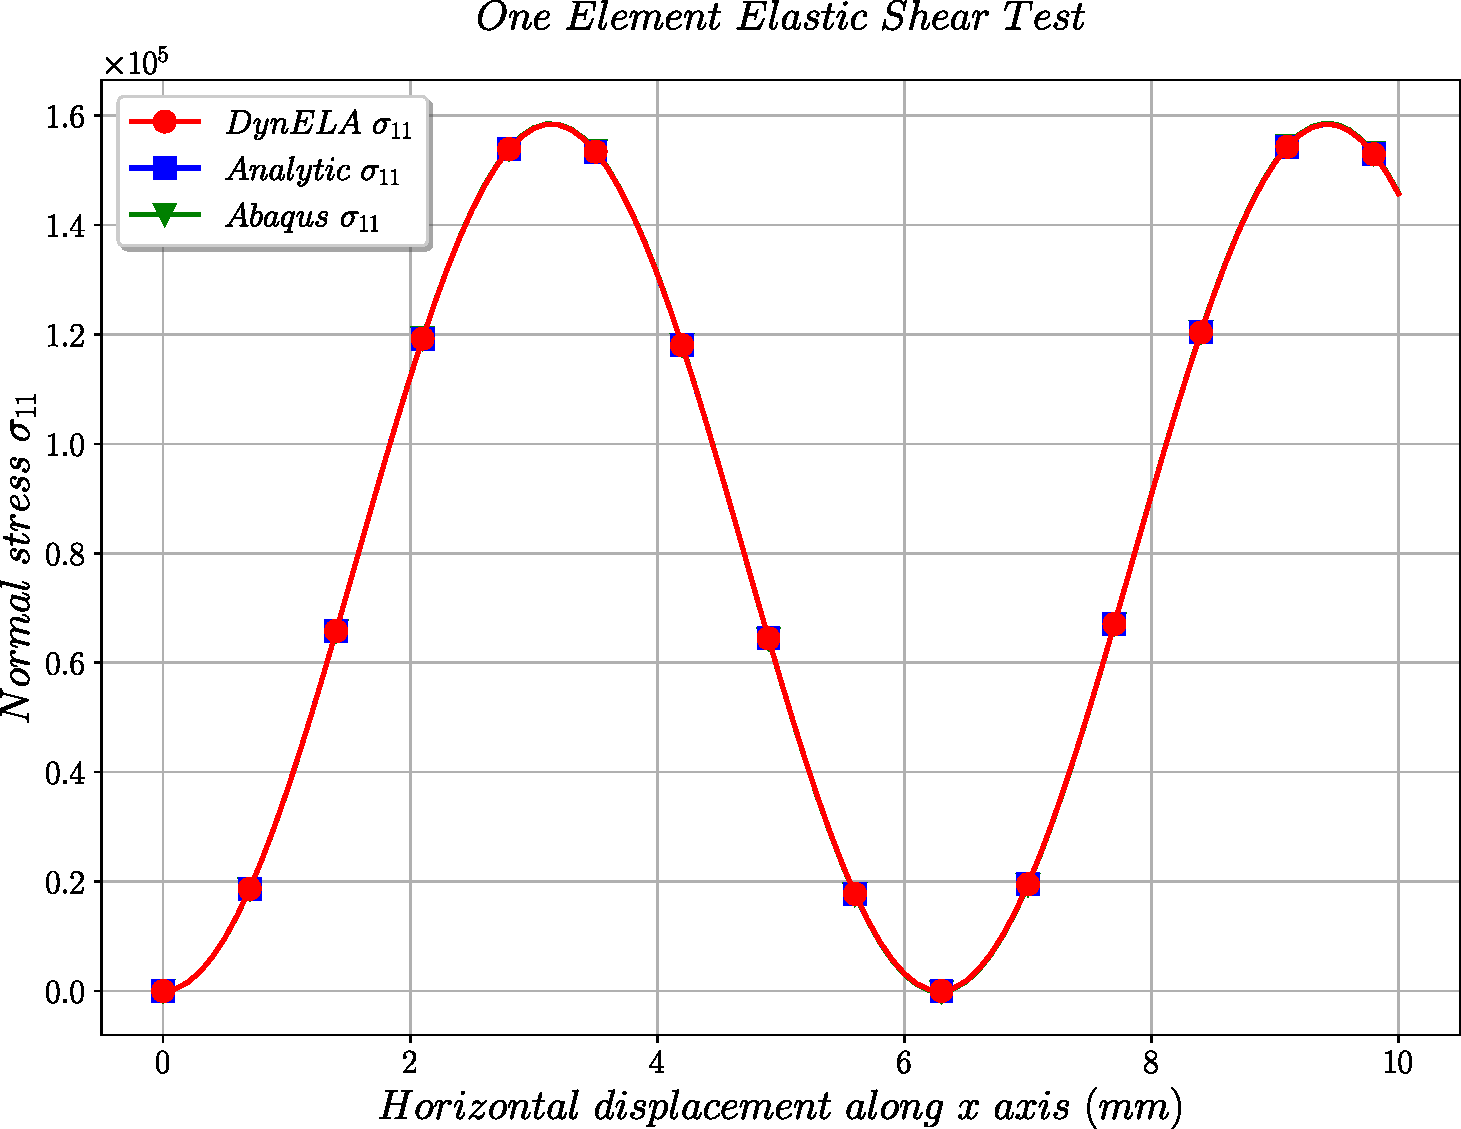
\includegraphics[width=0.45\columnwidth]{Figures/Samples/Element/Shear-Elastic_stress_11} & 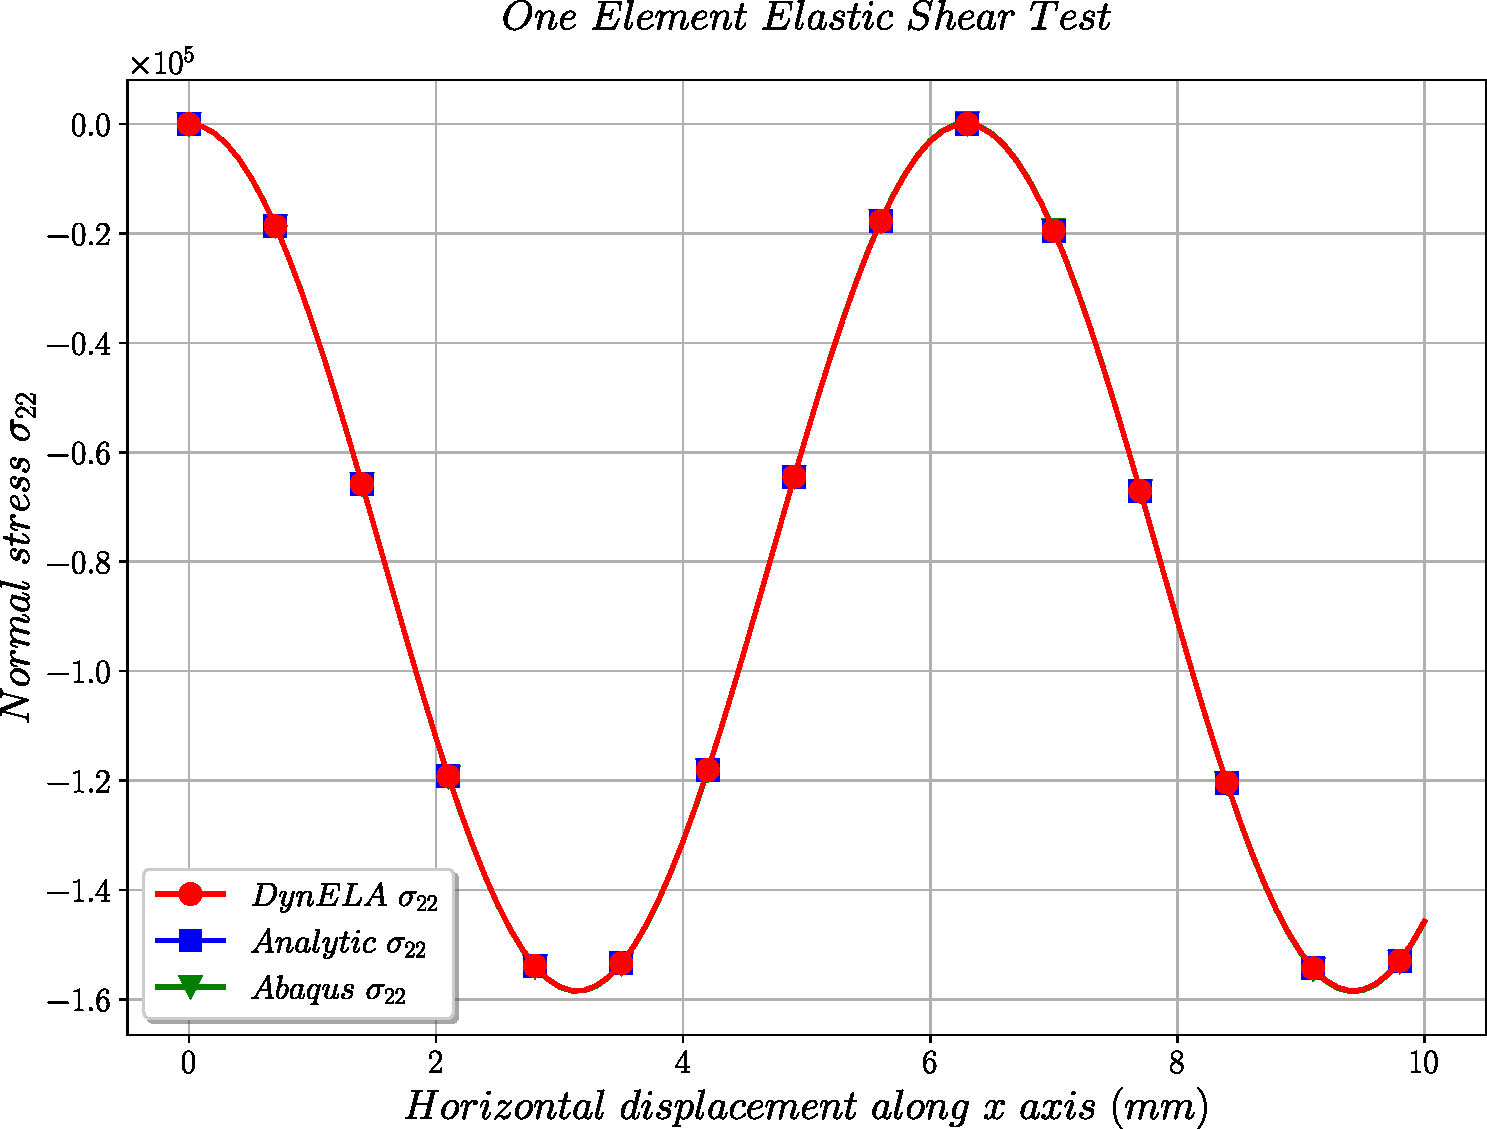
\includegraphics[width=0.45\columnwidth]{Figures/Samples/Element/Shear-Elastic_stress_22}\tabularnewline
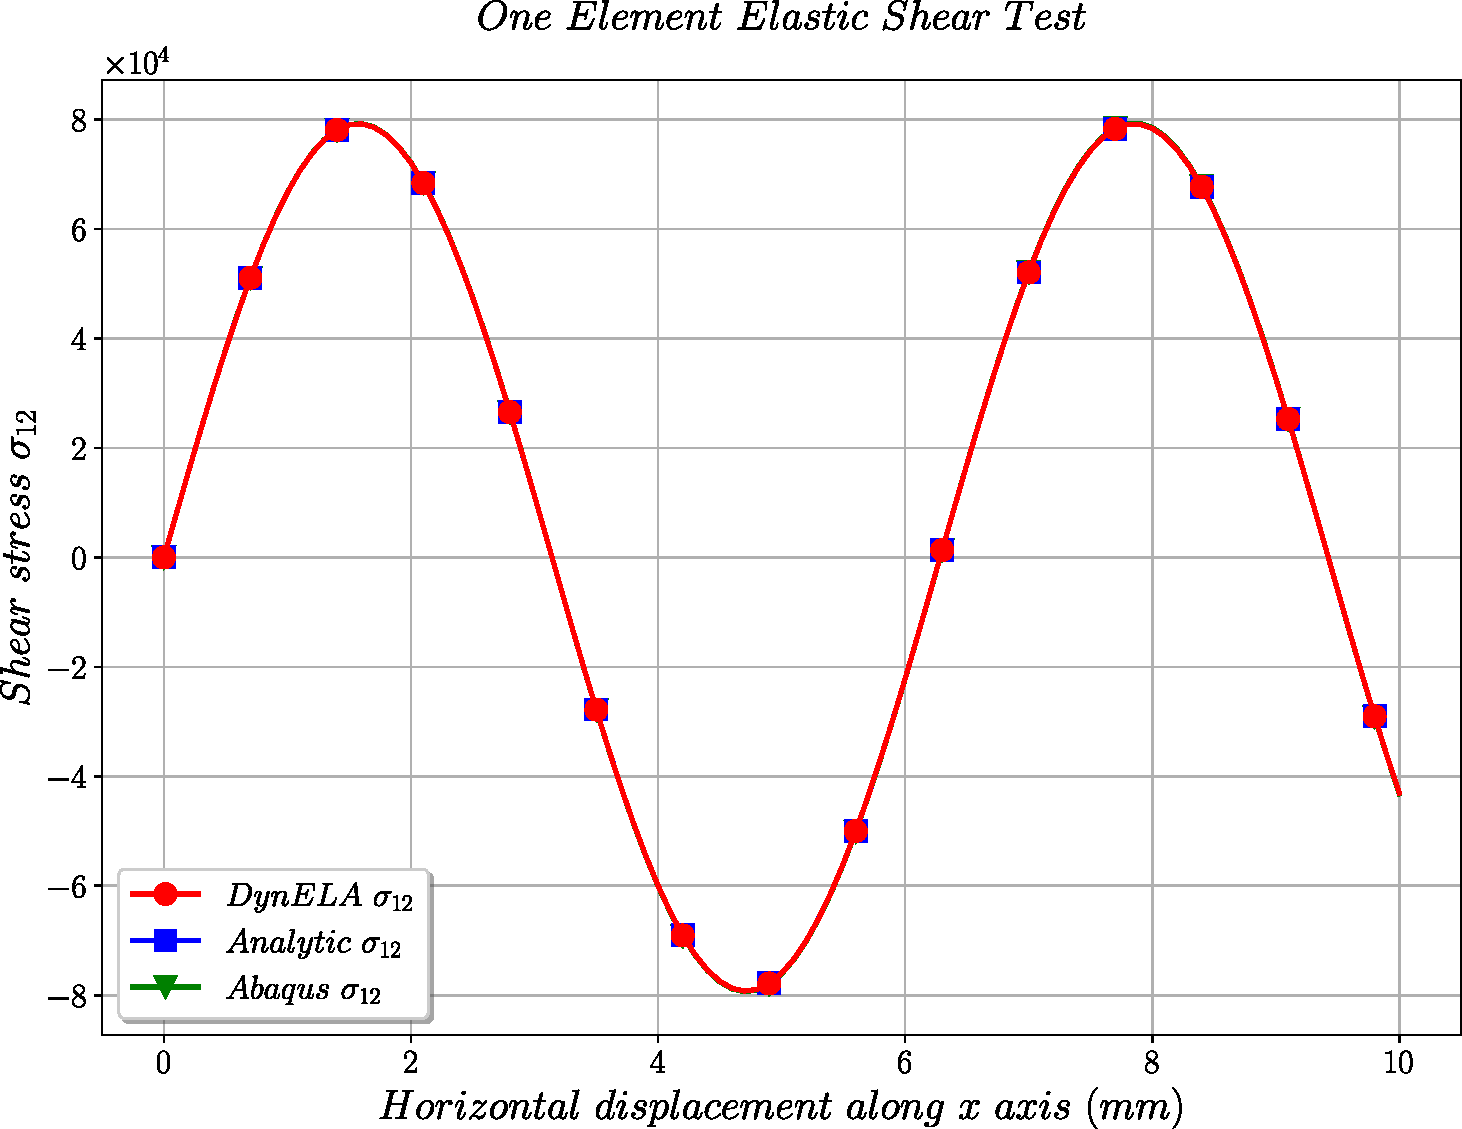
\includegraphics[width=0.45\columnwidth]{Figures/Samples/Element/Shear-Elastic_stress_12} & 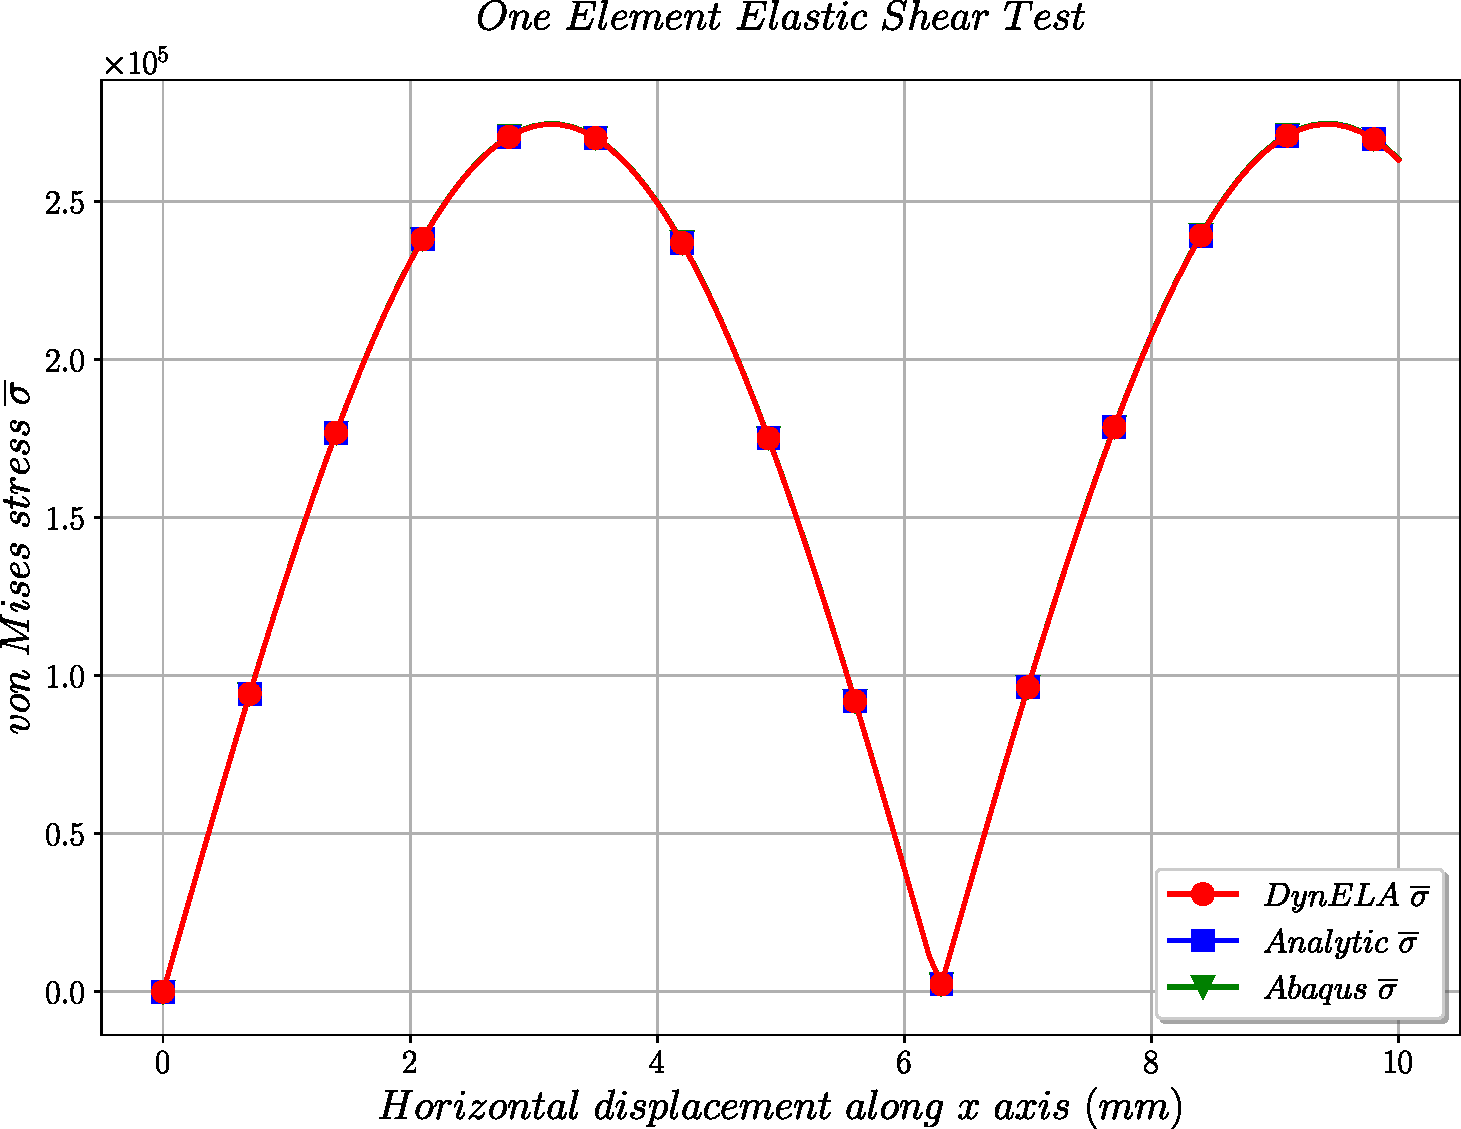
\includegraphics[width=0.45\columnwidth]{Figures/Samples/Element/Shear-Elastic_vonMises}\tabularnewline
\end{tabular}
\par\end{centering}
\caption{Comparison of numerical and analytical results for the one element
elastic shear test\label{fig:Samples!Single!Shear-Elastic-Comparison}}
\end{figure}
\clearpage

\subsection{Johnson-Cook plastic behaviour}

In this case, all the properties of the constitutive law reported
in Table \ref{tab:Samples!JohnsonCookParameters} are used and the
material is assumed to follow the Johnson-Cook behavior described
by equation \ref{eq:Samples!Johnson-Cook}. Figure \ref{fig:Samples!Single!Shear-Comparison}
shows the comparison of the DynELA solver results (plotted in red)
and the Abaqus numerical results (plotted in blue) concerning the
evolution of the stress components $\sigma_{11}$, $\sigma_{22}$,
$\sigma_{12}$, $\overline{\sigma}$, $\overline{\varepsilon}^{p}$
and $T$ \versus  the horizontal displacement of the top edge of
the specimen along the horizontal axis.

\begin{figure}[h]
\begin{centering}
\begin{tabular}{cc}
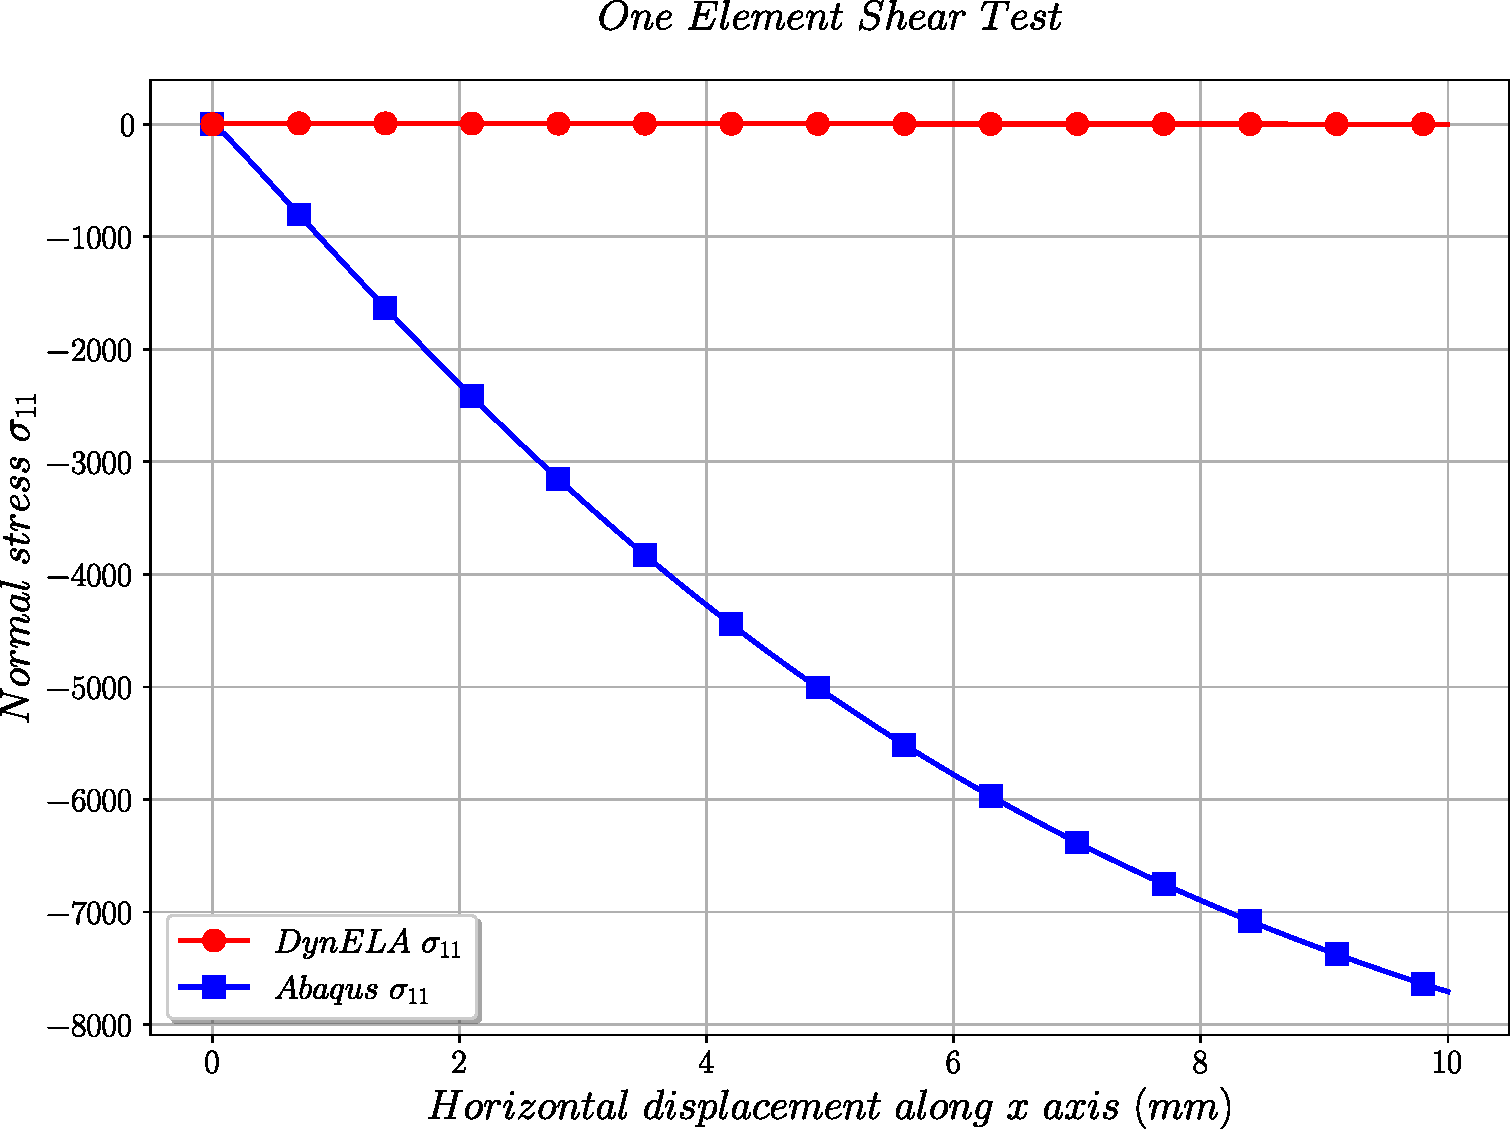
\includegraphics[width=0.45\columnwidth]{Figures/Samples/Element/Shear-Plastic_stress_11} & 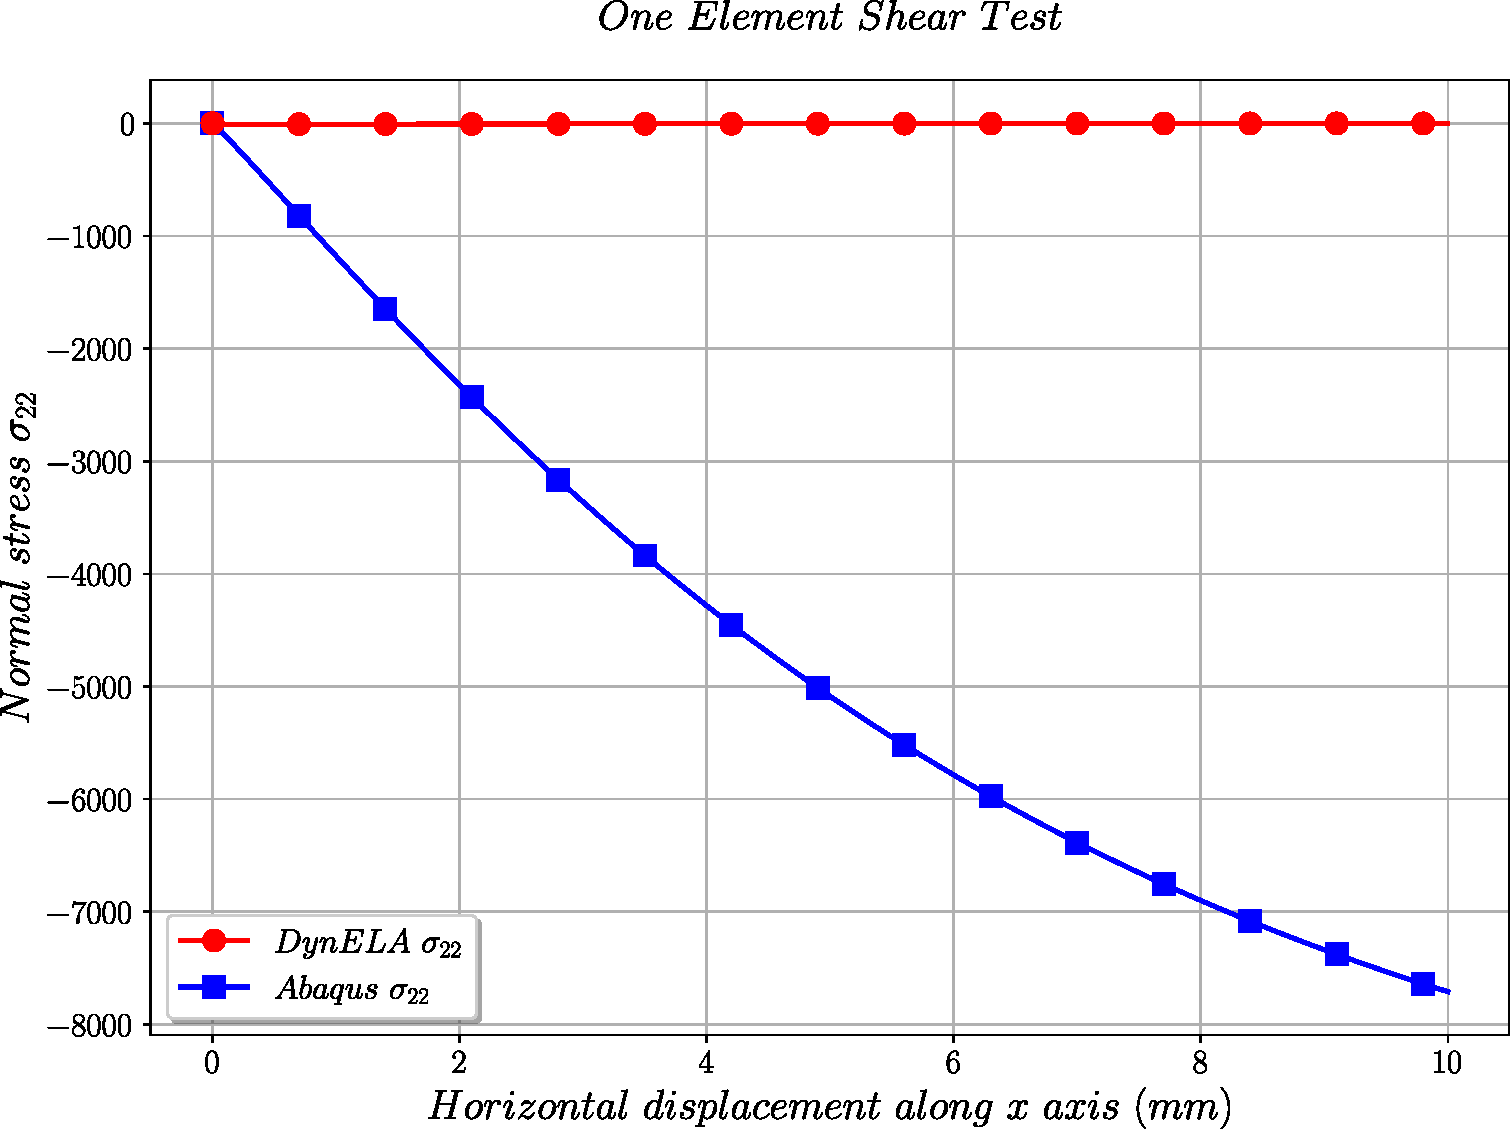
\includegraphics[width=0.45\columnwidth]{Figures/Samples/Element/Shear-Plastic_stress_22}\tabularnewline
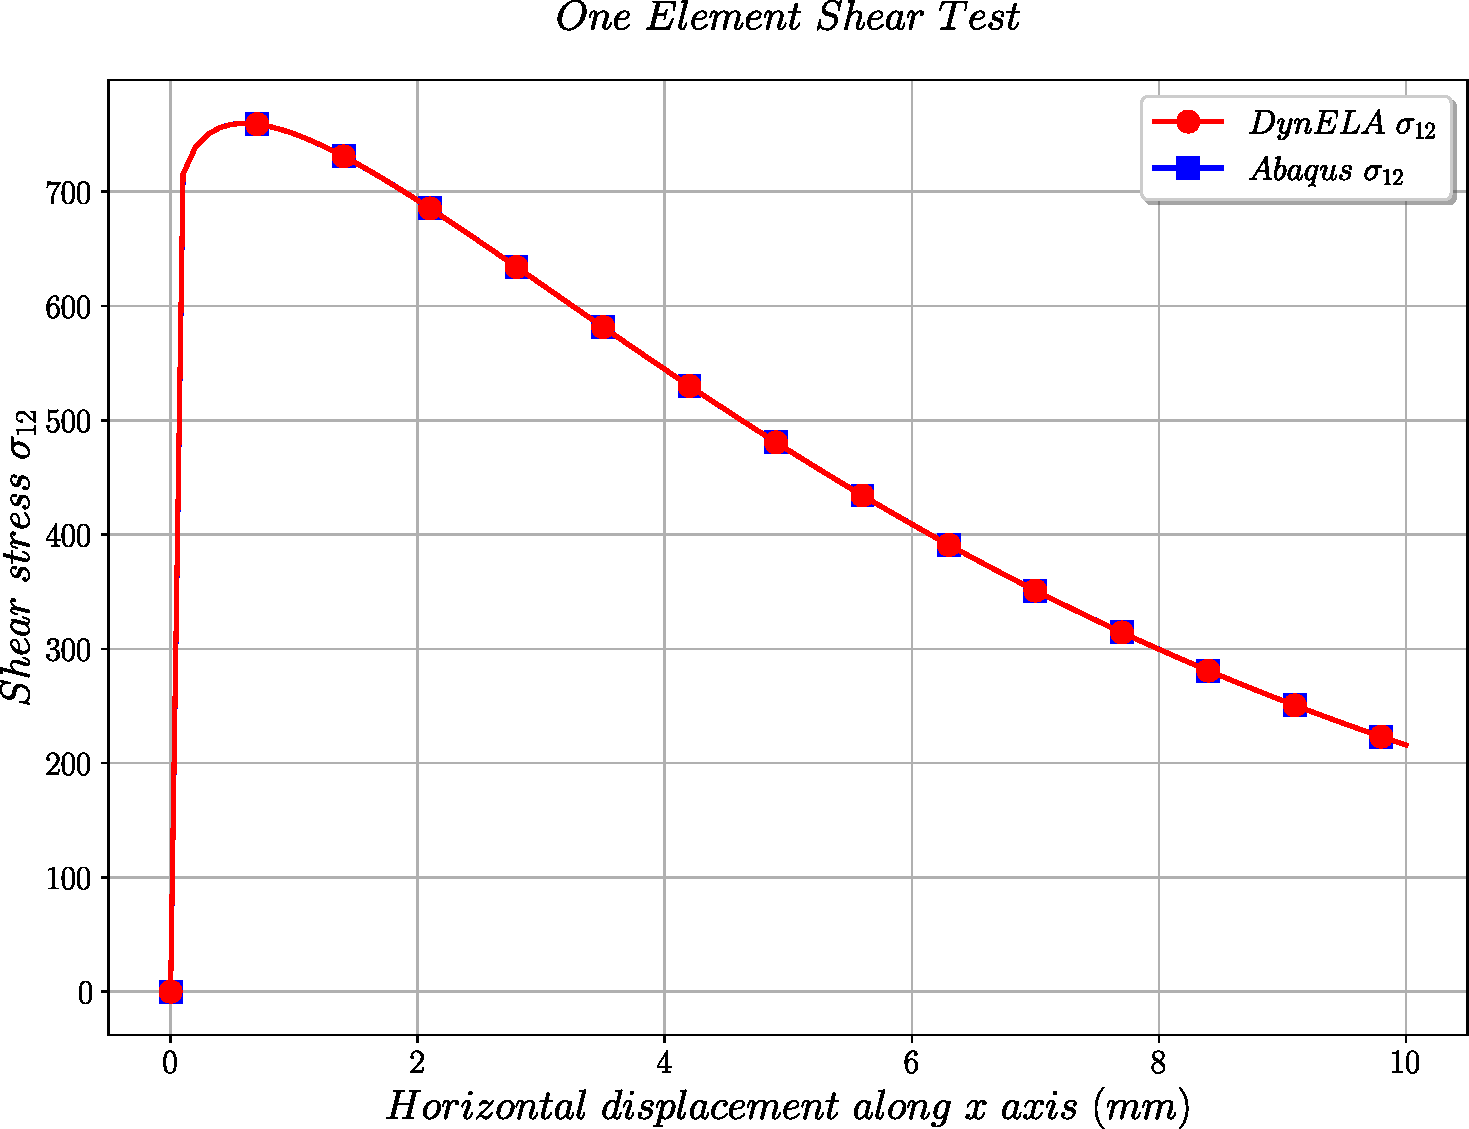
\includegraphics[width=0.45\columnwidth]{Figures/Samples/Element/Shear-Plastic_stress_12} & 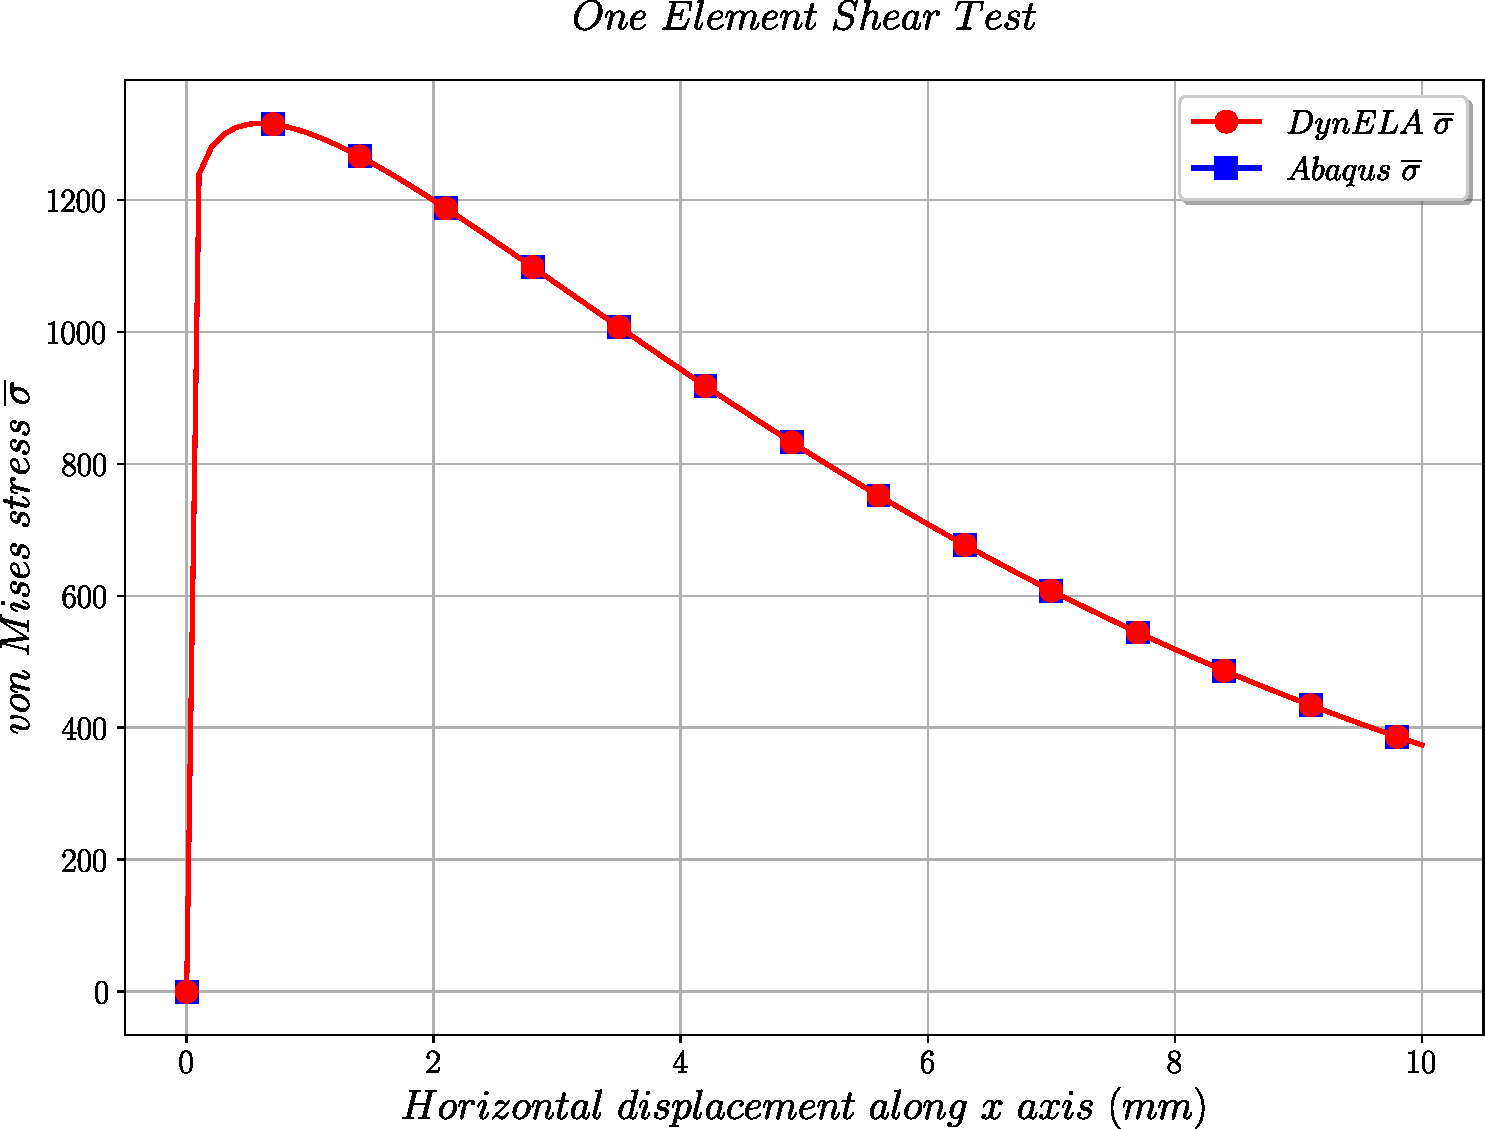
\includegraphics[width=0.45\columnwidth]{Figures/Samples/Element/Shear-Plastic_vonMises}\tabularnewline
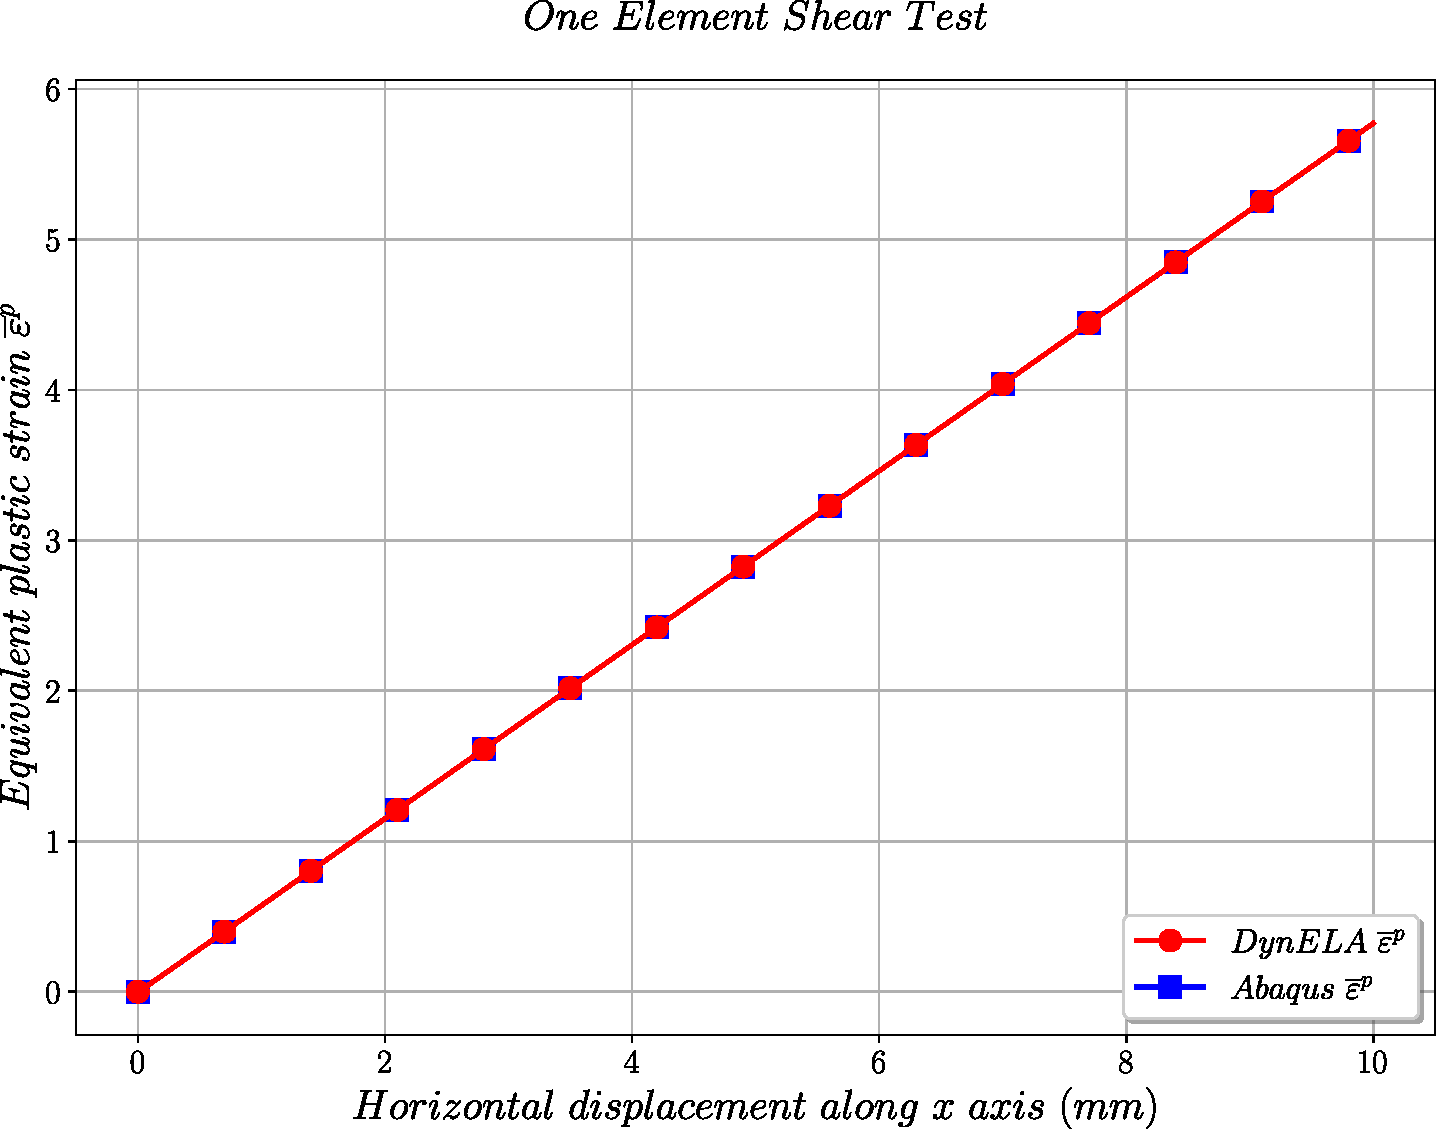
\includegraphics[width=0.45\columnwidth]{Figures/Samples/Element/Shear-Plastic_plasticStrain} & 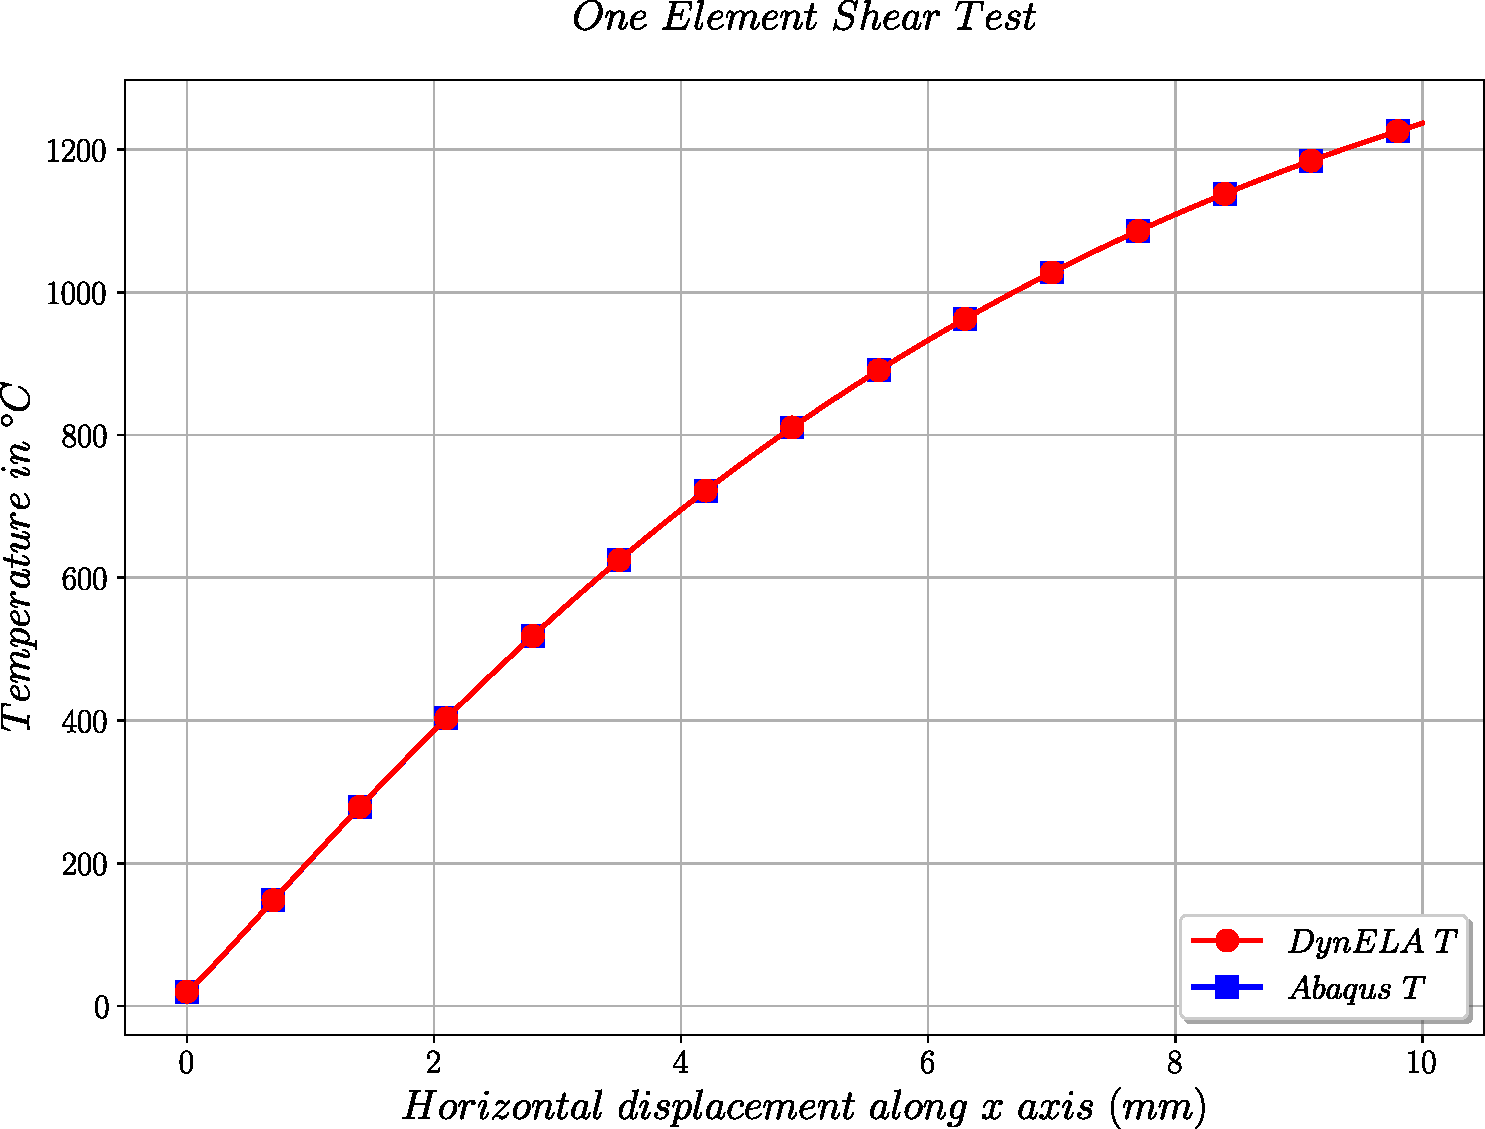
\includegraphics[width=0.45\columnwidth]{Figures/Samples/Element/Shear-Plastic_temperature}\tabularnewline
\end{tabular}
\par\end{centering}
\caption{Comparison of numerical and analytical results for the one element
shear test\label{fig:Samples!Single!Shear-Comparison}}
\end{figure}



% !TeX spellcheck = en_US
% !TeX root = DynELA.tex
%
% LaTeX source file of DynELA FEM Code
%
% (c) by Olivier Pantalé 2020
%
\chapter{DynELA plasticity sample cases}

\startcontents[chapters]
\printmyminitoc[2]\LETTRINE{T}his chapter deals with some numerical applications of
the \DynELA for plasticity applications in 2D, axi-symmetric and
3D cases. In the subsequent tests, if not specified, a Johnson-Cook
constitutive law is used to model the behavior of the material. The
Johnson-Cook hardening flow law is probably the most widely used flow
law for the simulation of high strain rate deformation processes taking
into account plastic strain, plastic strain rate and temperature effects.
Since a lot of efforts have been made in the past to identify the
constitutive flow law parameters for many materials, it is implemented
in numerous Finite Element codes such as Abaqus \cite{abaqus20146}.
The general formulation of the Johnson-Cook law $\sigma^{y}(\overline{\varepsilon}^{p},\stackrel{\bullet}{\overline{\varepsilon}^{p}},T)$
is given by the following equation:

\begin{equation}
\sigma^{y}=\left(A+B\overline{\varepsilon}^{p^{n}}\right)\left[1+C\ln\left(\frac{\stackrel{\bullet}{\overline{\varepsilon}^{p}}}{\stackrel{\bullet}{\overline{\varepsilon}_{0}}}\right)\right]\left[1-\left(\frac{T-T_{0}}{T_{m}-T_{0}}\right)^{m}\right]\label{eq:Samples!Johnson-Cook}
\end{equation}
where $\stackrel{\bullet}{\overline{\varepsilon}_{0}}$ is the reference
strain rate, $T_{0}$ and $T_{m}$ are the reference temperature and
the melting temperature of the material respectively and $A$, $B$,
$C$, $n$ and $m$ are the five constitutive flow law parameters.
A 42CrMo4 steel following the Johnson-Cook behavior law has been selected
for all those tests, and material properties are reported in Table
\ref{tab:Samples!JohnsonCookParameters}.

\begin{table}[h]
\begin{center}\begin{tcolorbox}[width=.75\textwidth,myTab,tabularx={C|C|C|C|C|C|C}]
$E$ & $\nu$ & $A$ & $B$ & $C$ & $n$ & $m$ \\
\small{($Gpa$)} &  & \small{($MPa$)} & \small{($MPa$)} &  &  & \\ \hline
$206.9$ & $0.3$ & $806$ & $614$ & $0.0089$ & $0.168$ & $1.1$ \\ \hline\hline
$\rho$ & $\lambda$ & $C_{p}$ & $\eta$ & $\stackrel{\bullet}{\overline{\varepsilon}_{0}}$ & $T_{0}$ & $T_{m}$ \\
\small{$(kg/m^{3})$} & \small{$(W/m^{\circ}C)$} & \small{$(J/Kg^{\circ}C)$} & & \small{$(s^{-1})$} & \small{$(^{\circ}C)$} & \small{$(^{\circ}C)$} \\ \hline
$7830$ & $34.0$ & $460$ & $0.9$ & $1.0$ & $20$ & $1540$
\end{tcolorbox}\end{center}\caption{Material parameters of the Johnson-Cook behavior for the numerical
tests\label{tab:Samples!JohnsonCookParameters}}
\end{table}


\section{Necking of a circular bar}

\subsection{Axisymmetric Bar Necking}

The necking of a circular bar test is useful to evaluate the performance
of VUMAT subroutine for materials in presence of plasticity and large
deformation \cite{ponthot_unified_2002, j_c_simo_computational_1998}. Because of the symmetric
structure, an axisymmetric quarter model of the specimen is established.
Dimensions of the specimen are reported in Figure \ref{fig:Samples!Plasticity!NeckingAxi}.
The loading is realized through an imposed total displacement of $7\,mm$
along the $\overrightarrow{z}$ axis on the left side of the specimen
while the radial displacement of the same edge is supposed to remain
zero. On the opposite side the axial displacement is restrained while
the radial displacement is free. The mesh consists of $400$ CAX4RT
elements with a refined zone of $200$ elements on the right side
on $1/3$ of the total height. Again, the total simulation time is
set to $t=0.01\,s$ because of the explicit integration scheme adopted.

\begin{figure}[h]
\begin{centering}
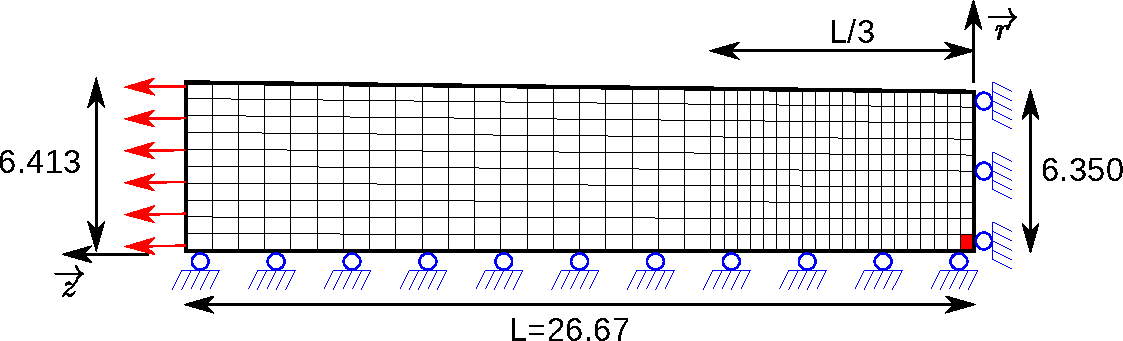
\includegraphics[width=0.75\columnwidth]{Figures/BarNecking}
\par\end{centering}
\caption{Numerical model for the necking of a circular bar\label{fig:Samples!Plasticity!NeckingAxi}}
\end{figure}

Figures \ref{fig:Samples!Plasticity!BarAxi-temp-contour} and \ref{fig:Samples!Plasticity!BarAxi-mises-contour}
shows the temperature $T$ and the von Mises stress $\overline{\sigma}$
contourplots of the deformed rod for both the \DynELA and Abaqus.
The distributions of the temperatures and stresses are almost the
same for both models. The maximum temperature $T$ is located into
the center element of the model (the red element in Figure \ref{fig:Samples!Plasticity!NeckingAxi})
and the models give quite the same results as reported in Table \ref{tab:Samples!Plasticity!BarAxi-comparison}
for $\overline{\varepsilon}^{p}$, $T$ and the final dimensions of
the specimen $D_{f}$ (final diameter of the necking zone).

Figure \ref{fig:Samples!Plasticity!BarAxi-comparison} shows the evolution
of the the final dimensions of the specimen $L_{f}$ (final length)
and $R_{f}$ (final radius of the impacting face), the equivalent
plastic strain $\overline{\varepsilon}^{p}$, the temperature $T$,
the von Mises stress $\overline{\sigma}$ and the timeStep $\Delta t$
for the different models for the element at the center of the impacting
face (the red element in Figure \ref{fig:Samples!Plasticity!NeckingAxi}).

As reported in this figure and according to the results presented
in Table \ref{tab:Samples!Plasticity!BarAxi-comparison}, a quite
good agreement between the results is obtained.

\begin{figure}[h]
\begin{centering}
\includegraphics[height=0.5\columnwidth]{Figures/Samples/Plasticity/BarNecking_temperatureCP}\hspace*{3cm}\includegraphics[height=0.5\columnwidth]{Figures/Samples/Plasticity/BarNecking-Abaqus_temperature}
\par\end{centering}
\caption{Temperature $T$ contourplot for the necking of a circular bar (DynELA
left and Abaqus right)\label{fig:Samples!Plasticity!BarAxi-temp-contour}}
\end{figure}

\begin{figure}[h]
\begin{centering}
\includegraphics[height=0.5\columnwidth]{Figures/Samples/Plasticity/BarNecking_vonMisesCP}\hspace*{3cm}\includegraphics[height=0.5\columnwidth]{Figures/Samples/Plasticity/BarNecking-Abaqus_vonMises}
\par\end{centering}
\caption{von Mises stress $\overline{\sigma}$ contourplot for the necking
of a circular bar (DynELA left and Abaqus right)\label{fig:Samples!Plasticity!BarAxi-mises-contour}}
\end{figure}

\begin{table}[h]
\begin{center}\begin{tcolorbox}[width=.75\textwidth,myTab,tabularx={C|C|C|C}]
code & $D_f$ & $T$ & $\overline{\varepsilon}^{p}$ \\
 & \small{($mm$)} & \small{($^{\circ}C$)} & \\ \hline\hline
DynELA & $2.71$ & $642.78$ & $2.07$ \\ \hline
Abaqus & $2.35$ & $658.91$ & $2.12$
\end{tcolorbox}\end{center}\caption{Comparison of numerical results for the necking of a circular bar
test\label{tab:Samples!Plasticity!BarAxi-comparison}}
\end{table}

\begin{figure}[h]
\begin{centering}
\begin{tabular}{cc}
\includegraphics[width=0.45\columnwidth]{Figures/Samples/Plasticity/BarNecking_radius} & \includegraphics[width=0.45\columnwidth]{Figures/Samples/Plasticity/BarNecking_kineticEnergy}\tabularnewline
\includegraphics[width=0.45\columnwidth]{Figures/Samples/Plasticity/BarNecking_temperature} & \includegraphics[width=0.45\columnwidth]{Figures/Samples/Plasticity/BarNecking_plasticStrain}\tabularnewline
\includegraphics[width=0.45\columnwidth]{Figures/Samples/Plasticity/BarNecking_vonMises} & \includegraphics[width=0.45\columnwidth]{Figures/Samples/Plasticity/BarNecking_timeStep}\tabularnewline
\end{tabular}
\par\end{centering}
\caption{Comparison of numerical and analytical results necking of a circular
bar test\label{fig:Samples!Plasticity!BarAxi-comparison}}
\end{figure}



% !TeX spellcheck = en_US
% !TeX root = DynELA.tex
%
% LaTeX source file of DynELA FEM Code
%
% (c) by Olivier Pantalé 2020
%
\chapter{DynELA impact sample cases}

\startcontents[chapters]
\printmyminitoc[1]\LETTRINE{T}his chapter deals with some numerical applications of
the \DynELA for impact applications in 2D, axi-symmetric and 3D
cases. In the subsequent tests, if not specified, a Johnson-Cook constitutive
law is used to model the behavior of the material. The Johnson-Cook
hardening flow law is probably the most widely used flow law for the
simulation of high strain rate deformation processes taking into account
plastic strain, plastic strain rate and temperature effects. Since
a lot of efforts have been made in the past to identify the constitutive
flow law parameters for many materials, it is implemented in numerous
Finite Element codes such as Abaqus \cite{abaqus20146}. The general
formulation of the Johnson-Cook law $\sigma^{y}(\overline{\varepsilon}^{p},\stackrel{\bullet}{\overline{\varepsilon}^{p}},T)$
is given by the following equation:

\begin{equation}
\sigma^{y}=\left(A+B\overline{\varepsilon}^{p^{n}}\right)\left[1+C\ln\left(\frac{\stackrel{\bullet}{\overline{\varepsilon}^{p}}}{\stackrel{\bullet}{\overline{\varepsilon}_{0}}}\right)\right]\left[1-\left(\frac{T-T_{0}}{T_{m}-T_{0}}\right)^{m}\right]\label{eq:Samples!Johnson-Cook}
\end{equation}
where $\stackrel{\bullet}{\overline{\varepsilon}_{0}}$ is the reference
strain rate, $T_{0}$ and $T_{m}$ are the reference temperature and
the melting temperature of the material respectively and $A$, $B$,
$C$, $n$ and $m$ are the five constitutive flow law parameters.
A 42CrMo4 steel following the Johnson-Cook behavior law has been selected
for all those tests, and material properties are reported in Table
\ref{tab:Samples!JohnsonCookParameters}.

\begin{table}[h]
\begin{center}\begin{tcolorbox}[width=.75\textwidth,myTab,tabularx={C|C|C|C|C|C|C}]
$E$ & $\nu$ & $A$ & $B$ & $C$ & $n$ & $m$ \\
\small{($Gpa$)} &  & \small{($MPa$)} & \small{($MPa$)} &  &  & \\ \hline
$206.9$ & $0.3$ & $806$ & $614$ & $0.0089$ & $0.168$ & $1.1$ \\ \hline\hline
$\rho$ & $\lambda$ & $C_{p}$ & $\eta$ & $\stackrel{\bullet}{\overline{\varepsilon}_{0}}$ & $T_{0}$ & $T_{m}$ \\
\small{$(kg/m^{3})$} & \small{$(W/m^{\circ}C)$} & \small{$(J/Kg^{\circ}C)$} & & \small{$(s^{-1})$} & \small{$(^{\circ}C)$} & \small{$(^{\circ}C)$} \\ \hline
$7830$ & $34.0$ & $460$ & $0.9$ & $1.0$ & $20$ & $1540$
\end{tcolorbox}\end{center}\caption{Material parameters of the Johnson-Cook behavior for the numerical
tests\label{tab:Samples!JohnsonCookParameters}}
\end{table}


\section{Taylor impact sample}

\subsection{Axisymmetric Taylor impact}

The performance of the proposed code is validated under high deformation
rate with the simulation of the Taylor impact test \cite{taylor_1946}.
In the Taylor impact test, a cylindrical specimen is launched to impact
a rigid target with a prescribed initial velocity. The numerical model,
reported in Figure \ref{fig:Samples!Impact!TaylorAxi} is established
as axisymmetric. The height is $32.4\,mm$ and the radius is $3.2\,mm$.
The axial displacement is restrained on the right side of the specimen
while the radial displacement is free (to figure a perfect contact
without friction of the projectile onto the target). A predefined
velocity of $V_{c}=287\,m/s$ is imposed on the specimen. The mesh
consists of $250$ elements ($5\times50$ elements). The total simulation
time for the Taylor impact test is $t=8.0\,10^{-5}s$.

\begin{figure}[h]
\begin{centering}
\includegraphics[width=0.75\columnwidth]{Figures/TaylorAxi}
\par\end{centering}
\caption{Numerical model for the Axisymmetric Taylor impact test\label{fig:Samples!Impact!TaylorAxi}}
\end{figure}

Figure \ref{fig:Samples!Impact!TaylorAxi-temp-contour} shows the
temperature contourplot of the deformed rod for both the \DynELA and
Abaqus. The distributions of the temperatures are almost the same
for both models. The maximum temperature $T$ is located into the
center element of the model (the red element in Figure \ref{fig:Samples!Impact!TaylorAxi})
and the models give quite the same results as reported in Table \ref{tab:Samples!Impact!TaylorAxi-comparison}
for $\overline{\varepsilon}^{p}$, $T$ and the final dimensions of
the specimen $L_{f}$ (final length) and $D_{f}$ (final diameter
of the impacting face).

Figure \ref{fig:Samples!Impact!TaylorAxi-comparison} shows the evolution
of the the final dimensions of the specimen $L_{f}$ (final length)
and $R_{f}$ (final radius of the impacting face), the equivalent
plastic strain $\overline{\varepsilon}^{p}$, the temperature $T$,
the von Mises stress $\overline{\sigma}$ and the timeStep $\Delta t$
for the different models for the element at the center of the impacting
face (the red element in Figure \ref{fig:Samples!Impact!TaylorAxi}).

As reported in this figure and according to the results presented
in Table \ref{tab:Samples!Impact!TaylorAxi-comparison}, a quite good
agreement between the results is obtained.

\begin{figure}[h]
\begin{centering}
\includegraphics[height=0.5\columnwidth]{Figures/Samples/Impact/Taylor-Axi_temperatureCP}\hspace*{3cm}\includegraphics[height=0.5\columnwidth]{Figures/Samples/Impact/Taylor-Axi-Abaqus_Temperature}
\par\end{centering}
\caption{Temperature contourplots for Axisymmetric Taylor impact test (DynELA
left and Abaqus right)\label{fig:Samples!Impact!TaylorAxi-temp-contour}}
\end{figure}

\begin{table}[h]
\begin{center}\begin{tcolorbox}[width=.75\textwidth,myTab,tabularx={C|C|C|C|C}]
code & $L_f$ & $D_f$ & $T$ & $\overline{\varepsilon}^{p}$ \\
 & \small{($mm$)} & \small{($mm$)} & \small{($^{\circ}C$)} & \\ \hline\hline
DynELA & $26.52$ & $11.15$ & $582.34$ & $1.78$ \\ \hline
Abaqus & $26.56$ & $11.16$ & $590.96$ & $1.81$
\end{tcolorbox}\end{center}\caption{Comparison of numerical results for the Axisymmetric Taylor impact
test\label{tab:Samples!Impact!TaylorAxi-comparison}}
\end{table}

\begin{figure}[h]
\begin{centering}
\begin{tabular}{cc}
\includegraphics[width=0.45\columnwidth]{Figures/Samples/Impact/Taylor-Axi_radius} & \includegraphics[width=0.45\columnwidth]{Figures/Samples/Impact/Taylor-Axi_height}\tabularnewline
\includegraphics[width=0.45\columnwidth]{Figures/Samples/Impact/Taylor-Axi_temperature} & \includegraphics[width=0.45\columnwidth]{Figures/Samples/Impact/Taylor-Axi_plasticStrain}\tabularnewline
\includegraphics[width=0.45\columnwidth]{Figures/Samples/Impact/Taylor-Axi_vonMises} & \includegraphics[width=0.45\columnwidth]{Figures/Samples/Impact/Taylor-Axi_timeStep}\tabularnewline
\end{tabular}
\par\end{centering}
\caption{Comparison of numerical and analytical results for the Axisymmetric
Taylor impact test\label{fig:Samples!Impact!TaylorAxi-comparison}}
\end{figure}


\subsection{3D Taylor impact}

The performance of the proposed code is validated under high deformation
rate with the simulation of the Taylor impact test \cite{taylor_1946}.
In the Taylor impact test, a cylindrical specimen is launched to impact
a rigid target with a prescribed initial velocity. The numerical model,
reported in Figure \ref{fig:Samples!Impact!Taylor3D} is established
as axisymmetric. The height is $32.4\,mm$ and the radius is $3.2\,mm$.
The axial displacement is restrained on the right side of the specimen
while the radial displacement is free (to figure a perfect contact
without friction of the projectile onto the target). A predefined
velocity of $V_{c}=287\,m/s$ is imposed on the specimen. The mesh
consists of $4455$ elements ($55\times81$ elements). The total simulation
time for the Taylor impact test is $t=8.0\,10^{-5}s$.

\begin{figure}[h]
\begin{centering}
\includegraphics[width=0.5\columnwidth]{Figures/Samples/Impact/Taylor-3D_mesh}
\par\end{centering}
\caption{Numerical model for the 3D Taylor impact test\label{fig:Samples!Impact!Taylor3D}}
\end{figure}

Figure \ref{fig:Samples!Impact!Taylor3D-temp-contour} shows the temperature
contourplot of the deformed rod for both the \DynELA and Abaqus.
The distributions of the temperatures are almost the same for both
models. The maximum temperature $T$ is located into the center element
of the model (the red element in Figure \ref{fig:Samples!Impact!Taylor3D})
and the models give quite the same results as reported in Table \ref{tab:Samples!Impact!Taylor3D-comparison}
for $\overline{\varepsilon}^{p}$, $T$ and the final dimensions of
the specimen $L_{f}$ (final length) and $D_{f}$ (final diameter
of the impacting face).

Figure \ref{fig:Samples!Impact!Taylor3D-comparison} shows the evolution
of the the final dimensions of the specimen $L_{f}$ (final length)
and $R_{f}$ (final radius of the impacting face), the equivalent
plastic strain $\overline{\varepsilon}^{p}$, the temperature $T$,
the von Mises stress $\overline{\sigma}$ and the timeStep $\Delta t$
for the different models for the element at the center of the impacting
face (the red element in Figure \ref{fig:Samples!Impact!Taylor3D}).

As reported in this figure and according to the results presented
in Table \ref{tab:Samples!Impact!Taylor3D-comparison}, a quite good
agreement between the results is obtained.

\begin{figure}[h]
\begin{centering}
\includegraphics[width=0.8\columnwidth]{Figures/Samples/Impact/Taylor-3D_temperatureCP}
\par\end{centering}
\caption{Temperature contourplot for the 3D Taylor impact test\label{fig:Samples!Impact!Taylor3D-temp-contour}}
\end{figure}

\begin{table}[h]
\begin{center}\begin{tcolorbox}[width=.75\textwidth,myTab,tabularx={C|C|C|C|C}]
code & $L_f$ & $D_f$ & $T$ & $\overline{\varepsilon}^{p}$ \\
 & \small{($mm$)} & \small{($mm$)} & \small{($^{\circ}C$)} & \\ \hline\hline
DynELA & $26.52$ & $11.18$ & $597.10$ & $1.84$ \\ \hline
Abaqus & $26.55$ & $11.22$ & $597.01$ & $1.84$
\end{tcolorbox}\end{center}\caption{Comparison of numerical results for the 3D Taylor impact test\label{tab:Samples!Impact!Taylor3D-comparison}}
\end{table}

\begin{figure}[h]
\begin{centering}
\begin{tabular}{cc}
\includegraphics[width=0.45\columnwidth]{Figures/Samples/Impact/Taylor-3D_radius} & \includegraphics[width=0.45\columnwidth]{Figures/Samples/Impact/Taylor-3D_height}\tabularnewline
\includegraphics[width=0.45\columnwidth]{Figures/Samples/Impact/Taylor-3D_temperature} & \includegraphics[width=0.45\columnwidth]{Figures/Samples/Impact/Taylor-3D_plasticStrain}\tabularnewline
\includegraphics[width=0.45\columnwidth]{Figures/Samples/Impact/Taylor-3D_vonMises} & \includegraphics[width=0.45\columnwidth]{Figures/Samples/Impact/Taylor-3D_timeStep}\tabularnewline
\end{tabular}
\par\end{centering}
\caption{Comparison of numerical and analytical results for the 3D Taylor impact
test\label{fig:Samples!Impact!Taylor3D-comparison}}
\end{figure}



\cleardoublepage

\bibliographystyle{unsrt}
\addcontentsline{toc}{chapter}{\bibname}

\begin{center}
\includegraphics[width=0.4\columnwidth]{Figures/Bibliography}
\par\end{center}

\bibliography{Private,Bibliography}

\cleardoublepage

\printindex
\printindex[PL]
\end{document}
